% arara: pdflatex: { synctex: on } 
% arara: pdflatex: { synctex: on } 

\documentclass[oneside]{scrbook} 

\usepackage[usenames, dvipsnames]{color}
\usepackage{graphicx}
\usepackage{float}
\usepackage{amsfonts}
\usepackage{amsmath}

\title{The Elements of Data Science: A Perspective from Applied Statistics and Machine Learning} 
\author{Bin Yu, Rebecca Barter} 

%\publishers{School of Something\\University of Somewhere} 

\begin{document} 
\maketitle 

\frontmatter 




\chapter*{Introduction: Why study applied statistics}
\label{ch:intro}



Advances in information technology have made the process of collecting huge amounts of data not only possible, but also extremely easy. The massive quantities of data available in the modern era enable scientists, social scientists, government agencies and companies to ask and answer questions in order to understand the physical world, make pubic policies, and improve productivity. For example, data can now be used to provide answers to an extremely broad array of questions such as ``is there a link between alcohol and birth defects?'' and ``What effect does incarceration have on the probability of a re-offence?''. Statistics is an indispensable tool in the process of extracting meaningful answers to the questions being asked based on the collected data. In fact, statistics is more than an analysis tool: statistical experimental design provides principles and methods for ensuring that the data is collected in such a way that facilitates the investigators' ability to effectively address the questions asked.

The tools provided by statistics were first developed as instruments used to solve real-world problems such as demographic census collection and agricultural experiments. As the types of data being collected grew more intricate, detailed and complex, so too did the accompanying statistical methods and the assumptions upon which they are based. Consequently, analyzing a dataset with no real-world knowledge of how the data was collected or what the numbers represent is the equivalent to \textcolor{red}{some nice analogy}. 


To ensure that useful questions are asked and valid answers are drawn, domain experts (scientists, for example) should always be in the picture for statisticians to strengthen their domain knowledge by asking questions and brainstorming. Data does not stand alone: it must be viewed with a strong consideration towards the questions being asked, the scientific background of the problem and the data collection process.



\section*{What to expect from this book}

The primary purpose of this book is to demonstrate what it is like to use statistics in the real world and to how to work together with people who have domain expertise in order to do data analysis with the aim of answering questions outside statistics. As a reader of this book, you will gain insight into the many steps involved in the iterative process of extracting information from data for the purposes of prediction and interpretation. In particular, this book will provide the necessary background to cover basic useful statistical methods in practice and will highlight how judgement and common sense should be used in the process of data analysis and when arriving at valid conclusions. 

Statistical techniques will be introduced through a first-principles approach with a focus on developing intuition, and the reader will learn how to develop appropriate techniques in unfamiliar situations. A number of data analysis labs are provided which are designed to help the reader put into practice the techniques and intuition conveyed throughout the book.

These principles will be demonstrated in the context of an ongoing collaborative genomic \emph{Drosophila} fruitfly project I am working on with several of my students in statistics and my colleagues in the biological sciences. 

\section*{Who should read this book}

The reader of this book is assumed to be familiar with concepts typically introduced in upper division mathematical statistics and probability courses. Further, to get the most out of the labs, the reader is encouraged to have familiarity with writing functions, manipulating and cleaning data and creating graphics in a programming language such as R.

This book is ideal for those who are looking to learn how to connect statistics to the real world, not those who are seeking the "optimal" method for broad classes of problems. If you are familiar with statistical concepts but would like to further develop your ability to use common sense, judgement and critical thinking in statistics, then this book is for you.


\section*{Recommended reading}

There exist a number of excellent texts for learning the intuition behind and the application of statistics. We will touch on a few here, namely Statistical Models: Theory and Practice by David A. Freedman, the sentiments of which we have tried to echo in this book. Another great read (not just for those new to statistics, but also for the most seasoned analysts) is Statistics by David A. Freedman, Robert Pisani and Roger Purves. This book does a fantastic job of teaching statistics through connections to reality while managing to completely stay away from the mathematics all together. 
\tableofcontents 


\mainmatter 

\part{Applied Statistics: an introduction}



\chapter{How to be an applied statistician}
\label{ch:how}


In essence, this book is about how to be an applied statistician. More precisely, how to use the statistical methods you've picked up (be it through your degree or by necessity) in practice and collaboration. Before embarking on a journey discussing how to implement your statistical skills in reality, we will first spend some time discussing the tools that are necessary for one to be a successful applied statistician. In this section, we focus not on using statistical methods, but on the importance of thinking critically, communicating effectively and understanding the philosophy behind statistics.


\section{The importance of communication}

There is an unfortunate presumption that statisticians (along with mathematicians, computer scientists, etc) are terrible at communication. If you have great ideas or are doing inspirational work but lack the skills to adequately communicate it (not just to other statisticians, but also potential collaborators), then you will find it hard to make much of an impact. Modern mathematical and statistical education has equipped a generation that lacks awareness on the importance of being communicative, approachable and even likable, particularly for those who wish to work with non-statistician collaborators. 


Not only do we devalue verbal communication skills, but we also under-appreciate the importance of written communication skills. We focus so much on mastering the ``language of mathematics'' that we completely undermine our ability to portray our work to the outside world. Even our mathematical writing should have a narrative: words and imagery are just as important as equations, since your readers are much more likely to remember graphics and the overall story than theorems and formulae.


\section{Sources of data}

A common problem among statisticians is finding good sources of data. The truth is that in most cases we are not the ones who actually go and collect the data, and as a result those without collaborators turn to databases. The problem with this approach is that there is a lack of transparency about data taken from databases. For example suppose a neuroscientist collected some fMRI (functional MRI; brain imaging) data. It is likely that there were a number of pre-processing steps that were undertaken throughout this data collection procedure. For instance, not every brain is alike, and the images need to be co-registered to an anatomical space and then spatially-normalized (squashed and stretched to match some image template). The images are also blurred to accommodate the heterogeneity in individual anatomy. Finally the images are then typically converted to a matrix of numbers. Clearly the process of translating the original image to numeric data involved a large number of assumptions. If a statistician simply obtained their fMRI data from a database, they would be ignorant to the assumptions made and the pre-processing steps taken, each of which are significant sources of noise in the data. All they see is a matrix of numbers (or many matrices of numbers) but they do not know how those numbers arose from the experiment was undertaken which leads to the possibility of misinterpretation.

As exemplified above, it is extremely important to understand the experimental design including all pre-processing steps when analyzing data. It is vital to understand what the numbers in your dataset mean and how they were obtained. Moreover, if the experimental design was poor, then the statistician will be able to take this knowledge into consideration for their analysis and will know to approach with caution and take the conclusions generated with a grain of salt. Numbers are not magical; they can be severely misleading if their origin is ignored. The upshot of this discussion is that we should be weary of analyses performed on data taken from sources without knowledge of the data collection process.




\section{Sources of randomness in the data}

Whenever presented with a new dataset, it is good practice to begin by asking ``where did the randomness come from?''. Sometimes, the randomness is explicit; for example if it is from tossing a coin or simple random sampling, however, in most scenarios it is less black-and-white. Knowing the source of randomness can be extremely useful when the postulated model does not work.

It might help to carry out a thought experiment whereby you try to replicate the data collection process in order to identify possible sources of randomness, especially if you intend to postulate an observed dataset as realizations of random variables (as is assumed by most statistical models). For example, you might want to ask how you would go about collecting another set of data that share the same distribution as the data that you have already, or how would you replicate the experiment that generated the data that you have.

\section{Why should we shift away from the search for ``optimality''?}

It is an unfortunate truth that statistics has become a field obsessed with optimality. Although this may seem like a positive direction in theoretical statistics (why \emph{wouldn't} we want to find the method with the lowest risk or the quickest run-time?), in the world of applied statistics this push for optimality is resulting in a statistical philosophy that searches for the ``biggest'', ``best'' and ``fastest'' method, forgoing interpretability. Moreover, in the vast majority of situations in applied statistics there is no single optimal approach. By requiring optimality, even by defining optimality, we are constraining our freedom to solve the problem at hand. Firstly, how would one even define optimality in terms of an approach to an applied problem? It's not hard to identify good and bad approaches, but how can we specify that one single approach is ``optimal''? In my experience, I have never seen a data problem for which I feel I have found the ``optimal'' approach. Nothing is optimal in practice, we never truly satisfy the theoretical assumptions that guarantee optimality (for example, are our data ever really independent and identically distributed? probably not...). This lack of exactness in reality doesn't mean that we can't ``borrow'' some optimality from the theory, we just can't rely on it. It is important to look at the conditions; don't just look at the conclusions!

Even in most realms of theoretical statistical optimization (perhaps with the exception of convex optimization), quite often the result is not a globally optimal approach, but rather a local one.





\section{The accessability of statistics as a field}

With the emergence of data science as a field distinct from statistics, we should take this opportunity to ask why data science is not simply considered to be applied statistics. When people think of statistics, they think of t-tests, exuberant probability distributions, and limiting results with assumptions that never hold in reality. One of the aims of this book is to change this perspective, with the key message that, more than anything else, statisticians are problem solvers. One of the key issues is that, as a field, we tend to get so caught up in the assumptions and technical details of our theorems and models, sometimes to the extent that if we cannot prove what we are trying to show, we simply continue to make assumptions about the data until we can. If this is our attitude, then why don't we just \emph{assume} that the conclusion is true? Further, these technical details tend to be so restrictive and incomprehensible that we push away anyone who might potentially want to use our results, simply because they don't understand it! Just because something has a lot of theorems, notation and fancy equations, that doesn't mean that it is ``good''. What use is the theory if no one outside of the niche field in which it was produced can understand it?



\section{Critical thinking}

The need to move away from the search for an optimal solution may understandably leave you asking what type of solutions you should seek. This is where judgement comes in: it may seem contradictory to many of you with a traditional objective statistical or mathematical education, but in reality many of the decisions made in applied statistical projects are brought about by thinking critically about the problem and making judgement calls. There is no clear answer or end-point like those in the theoretical problems.

Many, if not most, applied statistical problems you will face in reality cannot necessarily be solved using straightforward traditional methods. As an applied statistician, you will be faced with non-conventional problems which will require you to think critically and creatively, rather than automatically. Since no two problems are the same, the kind of skills required for true applied statistics will, for most people, be much harder to learn than formulaic mathematical skills. These skills are significantly more subjective and non-linear; traits that make many people uncomfortable (particularly those who would much rather prove theorems).

Although this book focuses on taking a step back from the theory when tackling applied problems, it certainly not true that theory is useless! Far from it; good theorems are extremely useful, and are indepsensible to the development and advancement of statistics. In the modern academic realm, however, there is such an expectation to produce new theorems, that a large amount of theorems presented in papers today encompass a disconnect between the assumptions upon which they are based and the methods.

The traditional statistical education route encourages blind model-fitting without truly considering the appropriateness of the model you are fitting and the assumptions that such an model may make about your data. As George Box said:
\begin{quote}
``All models are wrong, but some are useful.''
\end{quote}


This is the view that we take in this book: there are no true models, but some can lead to insights and directions to take in our analysis. In general, the sample variance should override the model bias, otherwise the model becomes a misguiding force.


\section{Using statistics in real life}

We have now arrived at the point where we talk about the increasing disconnect between applying statistics in real life and learning (in a class, for example) about statistical methods. This section is in essence a justification for the entire existence of this book. 

If you've ever been in an applied statistics class, the chances are high that it went something like this:

\begin{enumerate}
\item ``Here's a new method! Let's learn how to derive it!''
\item ``It's homework time! Let's use this specific method we just learned how to derive on this pretty, clean and uninteresting dataset and report a p-value!''
\item Repeat steps 1-2 with new methods until the semester ends at which point you will be tested on whether you know how to derive the specific method and use each method when prompted on simple examples.
\end{enumerate}


If this was not your experience, congratulations; perhaps you learned something useful. The problem with the disturbingly common approach described above (ignoring, for the moment, issues with p-values) is that it bears virtually no connection to what it is really like to analyze data (also this approach can be really, really boring). Firstly, in the real world, there is typically no one to tell you what method to use and when. The general idea is to use what you know and then expand your search for a solution and learn new approaches. It is important to realize that within most classroom settings, you are deliberately given clean, doable problems. In reality, the data you encounter will most likely be messy, confusing and often the questions you ask may be impossible to answer using the data at hand. Statisticians need to be comfortable exploring data without guidelines; they need to gain ``data wisdom''.





\section{Data wisdom}

Data wisdom is ``the ability to combine domain, mathematical and methodological knowledge with experience, understanding, common sense, insight and good judgement in order to think critically about data and to make decisions based on data''. The essence of data wisdom can be encompassed in the following set of (not necessarily sequential) questions that a data analyst is encouraged to ask before embarking on and during any data analysis project.

\subsection*{1. Question}

It is important to explicitly formulate questions to ask. For example, in neuroscience: how does the brain work? Or in banking: to which group of customers should a bank promote a new service? This is where the domain experts come in. They will know which questions are important and how to properly formulate them. Interaction with domain experts is absolutely necessary for the success of the data science project to come.

\subsection*{2. Collection}

What are the most relevant data to collect to answer the question we are interested in exploring? If the analyst did not collect the data themselves, they should be asking how, when and where the data were collected and what the data is measuring. More explicitly, who collected the data? Over what time period? At what locations? What instruments were used?

\subsection*{3. Meaning}

Not only must we understand where the data came from, but also what it really measures. For example, it is surprisingly important to ask questions such as what does a number mean in the data? Does it measure what it was supposed to measure? How could things go wrong? What statistical assumptions is one making by assuming that things didn't go wrong?

\subsection*{4. Relevance}

Is the data collected relevant to answering the question formulated at the birth of the project? If not, what other data should one collect?

\subsection*{5. Translation}

The analyst must be able to translate the question being asked into a statistical setting. For example, if there are multiple possible translations (such as a translation into a prediction problem or a translation into an inference problem regarding a statistical model), which is the most appropriate? 

\subsection*{6. Comparability}

The analyst should assess the ability of the data to satisfy the assumptions made by the translation chosen in the previous step. For example, are the data units are comparable (you don't want to combine apples and oranges)? Do they need to be normalized? 

\subsection*{7. Visualization}

Visualization is an incredibly useful tool for assessing the suitability of both the data and statistical translation in answering the question at hand. Assessing plots of the data can reveal patterns, inconsistencies and unexpected data points that may require further examination. 

\subsection*{8. Randomness}

It is extremely important to identify where the randomness in the data comes from (for example, was it from the sampling procedure or a random treatment assignment mechanism?). The source of randomness in the data must correspond to the randomness assumed by the statistical model. 

\subsection*{9. Stability}

The next step is to explore the validity of the conclusions drawn. For example, do different methods yield the same qualitative conclusions? Do perturbations (perhaps by adding noise or subsampling exchangeable data units) change the conclusions drawn? Such checks are vital in ensuring reproducibility. 

\subsection*{10. Validation}

Finally, the conclusions should be explicitly tested through validation methods, such as by testing the conclusions on other kinds of data.



The concept of data wisdom is based on the notion of \emph{uncontrolled inspiration}: the approach by which we solve problems by first attempting a solution, then, if this solution is unsatisfactory, spending some time reading (or even better, talking to people) the relevant domain and statistical literature to draw inspiration for a new or modified approach, and repeating this process until we have a ``satisfactory'' solution (keeping in mind that there may be no such thing). Statisticians must be able to learn as they go along.

In this way, data analysis is like detective work: we first form a hypothesis and we then look for evidence in the data to support this hypothesis. Data analysis is also like peeling an onion. You peel one layer, and then another layer, and so on and so forth until you find what you're looking for. The only real difference between statistical data analysis and onions in that onions are guaranteed to have a finite number of layers.

\textcolor{red}{Above are three nice analogies (uncontrolled inspiration, detective, onion) -- probably choose one}



\section{Notes}

The egg-yolk study, \textit{egg yolk consumption and crotid plaque} was undertaken by Spence et al. (2012), and printed in the Elsevier journal of Atherosclerosis. 



 






\chapter{Ongoing projects}
\label{ch:projects}

I don't yet know where to put each of these project sections...

\section{The Drosophila fruitfly project}
Throughout this book we will embed many of the concepts we are discussing within a real-life project, which we will call ``the fruitfly project''. The fruitfly project is a genomics project that I have been involved in with several of my students and my collaborators at Lawrence Berkeley National Laboratory (LBNL).

As most do, the fruitfly project began with a question: ``Is spatial information useful for making gene-gene interaction discoveries?''. To expand and de-code this question for the non-biologists, what the group was really asking is whether it is possible to use stained images (more specifically, images of Drosophila embryos) to identify whether genes interact with one another. For an individual embryo, the staining process involves using dye to stain specific products that are produced when a particular gene is being expressed (these products are typically proteins). The upshot of the staining process is that areas within the embryo where the stain is visible correspond to physical locations within the embryo where the gene of interest is being expressed. 



With this question in mind, the group of biologists at LBNL had generated 1640 spatial gene expression images (see Figure~\ref{fig:embryo}) representing 755 genes for early \emph{Drosophila} embryos. In each image, the gene of interest is being expressed at the locations within the embryo where the blue stain is visible. Each processed expression image can be represented by a numeric vector with 405 entries, one for each of the 405 pixels inside the ellipse template.





\textcolor{red}{So the biologists had the data and the question but no idea how to answer it? They then invited Bin and co. to offer statistical insights whereby after much trial and error, we arrived at the non-negative matrix factorization approach. This approach allowed us to derive 21 principal patterns (PPs) using which we constructed spatially local correlation networks for all patterned transcription factors during early Drosophila development}

% img source: http://insitu.fruitfly.org/cgi-bin/ex/report.pl?ftype=1&ftext=TE18870

\begin{figure}[H]
\begin{center}
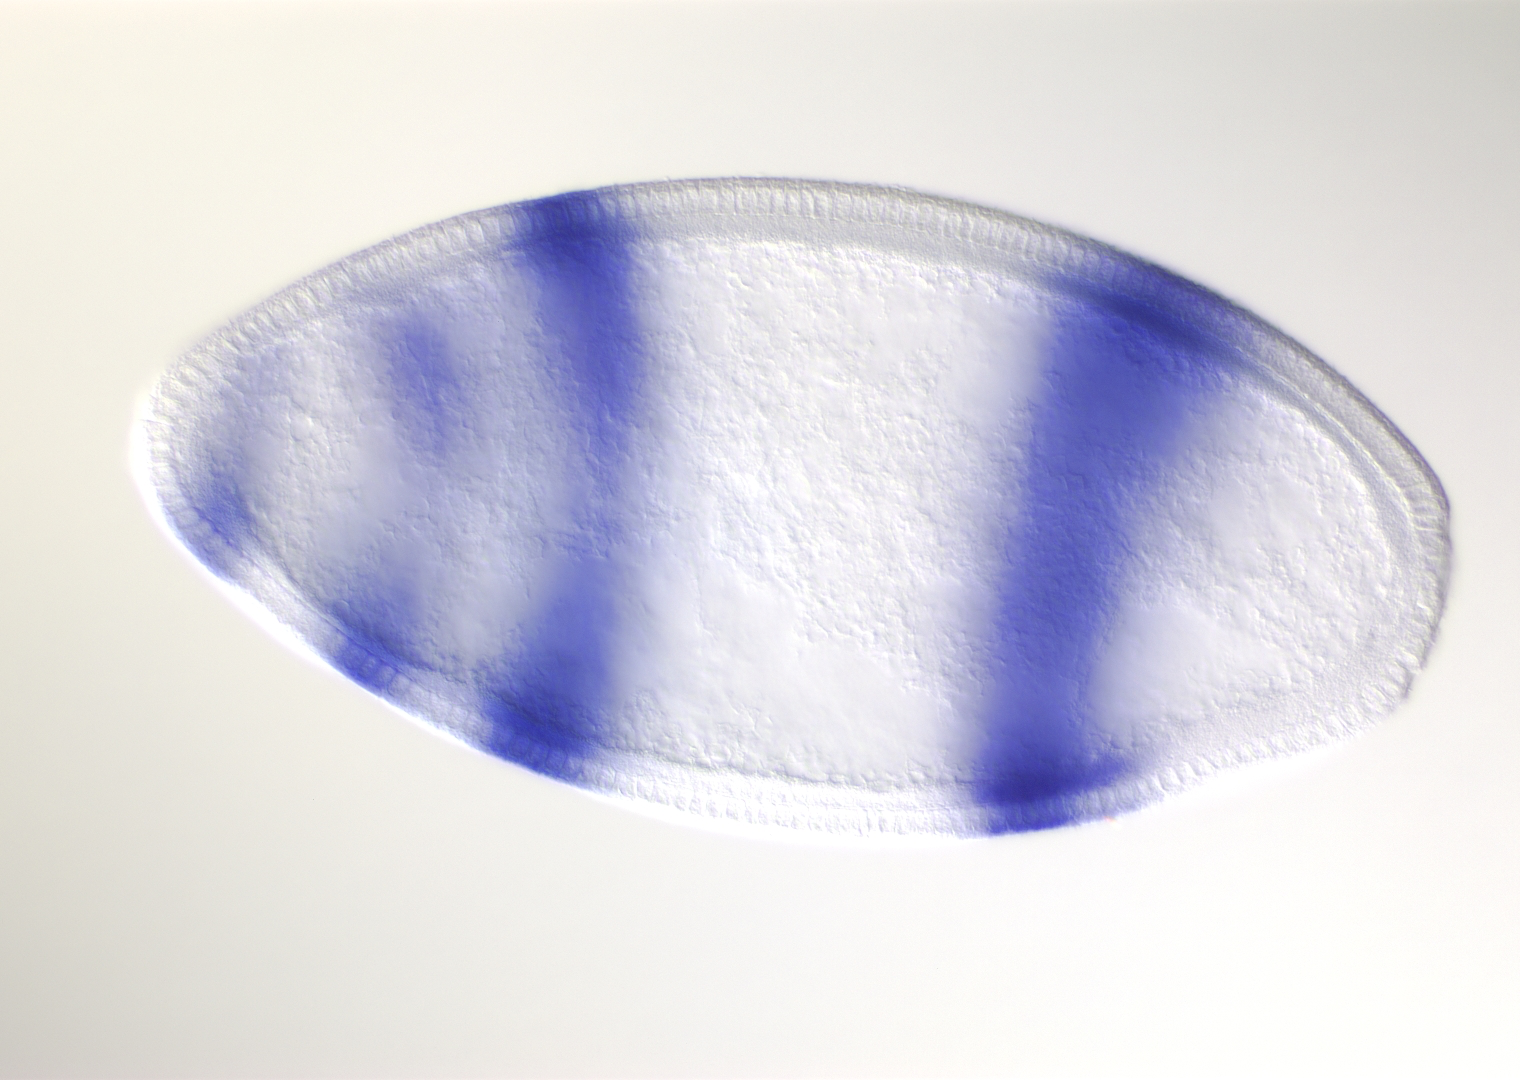
\includegraphics[scale=0.15]{embryo.png}
\end{center}
\caption{An example of drasophila embryo for which the blue stain corresponds to the regions of the embryo in which the \emph{giant} gene is being expressed.}
\label{fig:embryo}
\end{figure}


\subsection*{The gap gene network}

The gap gene network consists of a group of interacting genes each of which are involved in the process of segment determination in the early development stages of the fruitfly. discovered by Nobel Prize winners Christiane N\"{u}sslein-Volhard and Eric Wieschaus in 1980. The term ``gap'' arose as a result of the effect of mutations of these genes on the embryonic development: gap genes cause the loss of central segments from the embryo which results in gaps in the developing structure.

Examples of these genes include \emph{kr\"{u}ppel}, whose early expression domain is in the center of the embryo, which, along with \emph{knirps} and \emph{giant} are among the earliest genes expressed during development. These genes subdivide the embryo along the anterior/posterior axis (the longest axis).


\begin{figure}[H]
\begin{center}
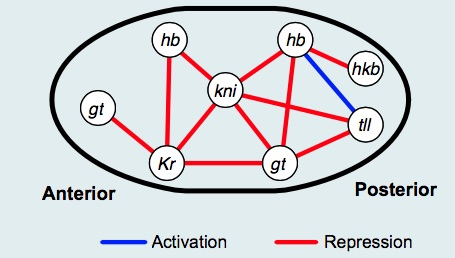
\includegraphics[scale=0.5]{gap_gene.jpg}
\end{center}
\caption{The gap gene network}
\label{fig:gap}
\end{figure}




In Figure~\ref{fig:gap} above, we see a network of 8 gap genes each of which have activation or repression effects on one another. For example, \emph{gt} (giant) and \emph{Kr} (Kr\"{u}ppel) repress one another in the sense that if \emph{Kr} is being highly expressed, then \emph{gt} will be less expressed. \emph{hb} (hunchback) and \emph{tll} (tailless), on the other hand, activate one another whereby increased expression of one of the genes activates increased expression of the other.


\begin{figure}[H]
\begin{center}
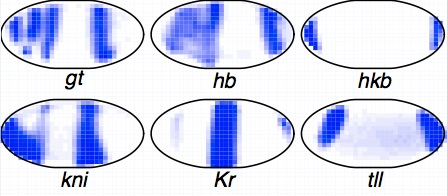
\includegraphics[scale=0.5]{embryos.jpg}
\end{center}
\caption{Expression regions for each of the gap genes}
\label{fig:stains}
\end{figure}


Figure~\ref{fig:stains} presents examples of embryos for which the product of the expression of each corresponding gap gene is dyed blue. That is, each image shows us the locations where (and extent to which) each gap gene is being expressed. We see that the \emph{Kr} (Kr\"{u}ppel) gene is expressed in the mid-region of the embryo, while \emph{hkb} (huckebein) gene is expressed only at the posterior and anterior ends. We also see that although there are regions of complementary expression, for example \emph{gt} and \emph{hb} have complementary expression patterns towards the right end of the embryo, implying that their local correlation is negative.





\subsection*{The experiment}

When we stained the products of the expression of \emph{new genes} with unknown functions in our embryos, we were able to use the images to identify whether these new genes interacted with the known gap genes.


\begin{figure}[H]
\begin{center}
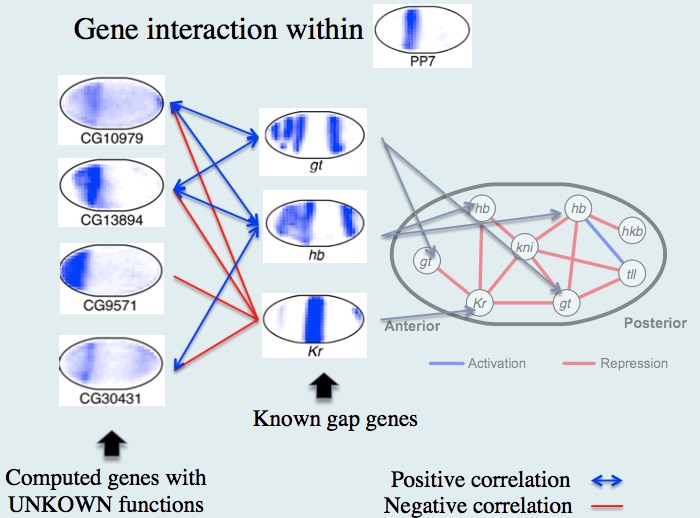
\includegraphics[scale=0.5]{embryos1.jpg}
\end{center}
\caption{Our new CG genes and the gap gene network}
\label{fig:embryo_gap}
\end{figure}



What we found was that our new genes (CG genes) interacted with the famous gap gene network. For example, two genes are positively correlated if they are expressed in the same location in the embryo (the genes have an activation relationship), and negative correlation if they are expressed in non-overlapping locations (the genes have a repressive relationship).

So the question became, are these new genes (focusing on the CG13894 gene) part of the gap gene network?

To answer this question, gene knock-out experiments were carried out by Ann Hammonds in Celniker's lab at LBNL. This is an experiment with an \emph{intervention}: in some embryos, we ``knock-out'' the gene of interest and observe the difference between the development of these embryos and normal embryos. This can be seen as a randomized experiment from which we can try to draw causal inferences \textcolor{red}{What are we trying to infer that knocking out this gene causes?}.

Our local analysis predicted that knocking out CG13894 would cause a change in the gap between the first two stripes \textcolor{red}{(what are these stripes -- is this still staining gene expression or is this just segmentation)}


We formulated this into a hypothesis that asked: ``Will knocking out CG13894 cause a narrowing in the gap between the first two stripes?'', a well formed question that we could assess using a randomized experiment: from our sample of embryos, we could randomly select a certain number to undergo the knock-out process (the treatment embryos) and allow the remainder to develop naturally (the control embryos). We could then compare the gab between the first two stripes between the two groups of embryos. Seems straight forward right? Maybe not... First of all, how can we quantitatively compare the gap between the stripes in a reliable way (i.e. other than by simply looking at them)?




\begin{itemize}
\item {\bf The first approach}: measure the gap between the stripes within the image. But embryos come in all different shapes and sizes! Recall our data wisdom section on ensuring comparability between our units of analysis. Comparability is extremely important in this situation, otherwise we have a confounding factor which is the size of the embryo. 
\item {\bf The second approach}: count the number of cells in the gap between the stripes. How could we automatically count the number of cells in images of this resolution? We had to manually count the number of cells which is tedious. Further, the count may be different at different ages, since as the development progresses, the cells divide, so we may just be counting the age of the embryo! Further, what if the change in the gap is a result of the cell size changing instead of the number of cells. Then this measure would be useless.
\end{itemize}




Even in measuring this gap, there are a lot of judgement calls and assumptions that come into play. For example, should we normalize? Stripes from each embryo are of different thicknesses and perhaps we should be considering the size of the gap relative to the size of the stripes for each embryo. The histograms below show the distances first when we do not normalize and then after normalizing relative to the size of the first stripe (the ratio of the size of the gap to the size of the stripe).


\begin{figure}[H]
\begin{center}
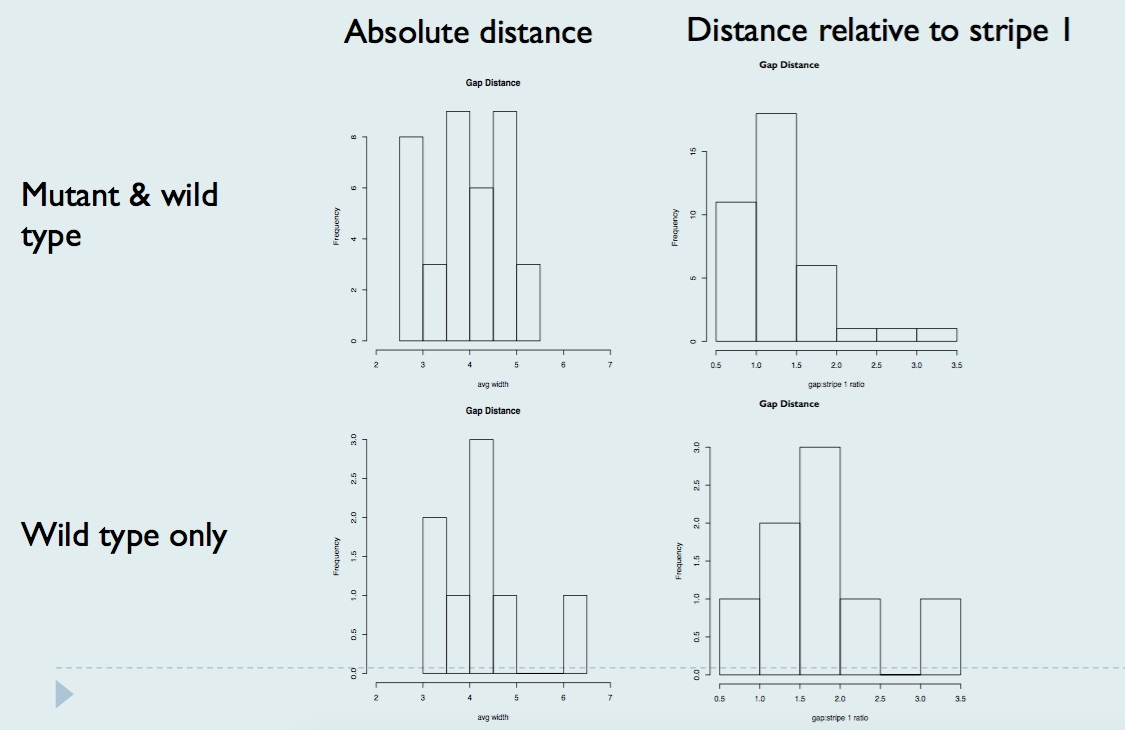
\includegraphics[scale=0.25]{gap_width.jpg}
\end{center}
\caption{Histogram of gap widths}
\label{fig:gap_widths}
\end{figure}



Perhaps you might now think about a few of our data wisdom questions from the previous chapter and apply them to this project:

\begin{enumerate} 
\item What does a number in this dataset mean? It is often not discussed enough what numbers are you actually interested in. Do the numbers you have actually measure what you're interested in. If you're using the wrong numbers, then you either don't see anything or you see things that aren't really there. We discussed above different types of ``numbers'' that we could have used for the distance. Some would have been more effective than others for detecting a real difference between the knock-out embryos and the control embryos.
\item Eventually you'll find a difference between the mutant and normal embryos. When this occurs, how can you test to see if this difference is real and not just an artefact of the data you have or the model you used? Instead of worrying about this problem at the end, it is always a good idea as soon as you've collected your data to set aside some subset (half?) of the data and don't use it for any of your analysis (this witheld subset of your data is called the \emph{test data}). You don't want to ``over-snoop'' the data. When you have a finding based on your training data, you can test to see whether the results are also true in the test data.
\item How was the randomization done in this experiment? We told you that the embryos were randomized to either undergo the knock-out procedure or not, but we didn't tell you how this occurred. 
\item What is our overall population? What are we assuming about the population? The embryos have all been bred in the lab and come from a particular genetic lineage. The population about which we are making inferences is not simply \emph{all fruitflies} in the world, or even in Berkeley. Even amongst the fruitflies at the lab, there is not overall homogeneity. Each embryo is different.
\item How was the knock-out ``intervention'' performed? It's certainly not possible to simply manipulate each individual fruitfly. Typically you perform the knock-out intervention in a few fruitflies and they pass the mutation on to their offspring. This process probably also resulted in many of the fruitflies dying, in which case, is there a difference between those who survived and those who died in terms of how extreme the gap difference would be?
\end{enumerate}
 
 
 
\section{The neuroscience project}
 
 
\subsection*{Neuroscience: Hubel and Wiesel's cat experiment}

Hubel and Wiesel (1959) conducted some of the pioneering research in showing how the visual system constructs complex representations of visual information from simple stimulus features. In one of their most notable experiments, they anesthetized a cat and propped its eyes open, so that the cat was physically seeing things, but was not conscious. They inserted a microelectrode into the primary visual cortex of the cat and they projected bright patterns (circle, line) on a dark screen in front of the cat. What they found was that some neurons fired rapidly when presented with lines at one angle, while others responded best to another angle. 


% https://goodpsychology.files.wordpress.com/2013/03/hubel-experiment.jpg

\begin{figure}[H]
\begin{center}
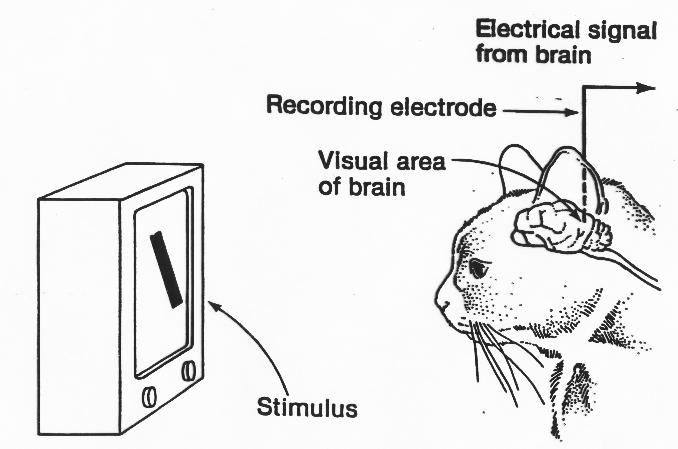
\includegraphics[scale=0.25]{hubel.jpg}
\end{center}
\caption{The Hubel and Wiesel cat experiment}
\label{fig:cat}
\end{figure}



This can be interpreted as a causal inference problem: placing the bright object in the line of view of the cat \emph{caused} the neurons to fire. This influential work was described by Professor David Ottoson of the Karolinsksi Institute as

\begin{quote}

``The signal message that the eye sends to the brain can be regarded as a secret code to which only the brain possesses the key and can interpret the message. Hubel and Wiesel have succeeded in breaking the code''
\end{quote}


There has been a recent new wave of research interest in the area of understanding how the brain processes visual stimuli, particularly utilizing deep learning algorithms. A modern direction that developed from Hubel-Wiesel's work in the way in which we computationally preprocess images for analysis. We use \emph{Gabor filters} to model simple cells in the visual cortex, so Gabor functions can be thought of as the mathematical representation of the perception in the human visual system.

Gabor filters (see image below) correspond to functions which represent the particular spatial frequencies, locations and orientations that were discovered by Hubel and Wiesel's cat experiment in 1959. When analyzing images, it is very common to decompose the image into the gabor functions for analysis.

\begin{figure}[H]
\begin{center}
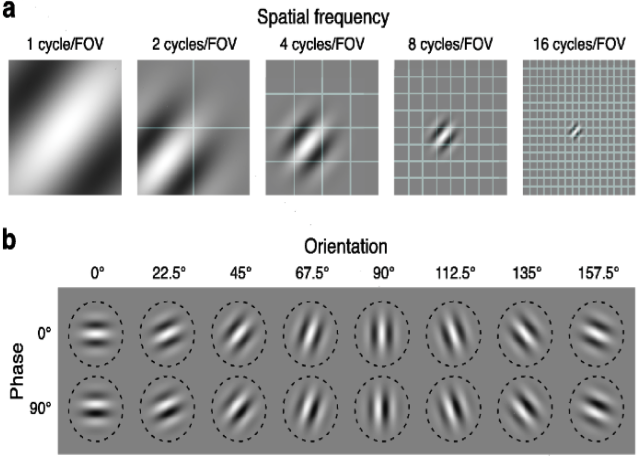
\includegraphics[scale=0.5]{gabor.png}
\end{center}
\caption{Gabor wavelets}
\label{fig:gabor}
\end{figure}


\subsection*{Movie reconstruction using fMRI data: The Gallant Lab}


This is a project that I was involved in with Jack Gallant's lab from the Redwood Center for Theoretical Neuroscience at UC Berkeley. The Gallant lab performed a number of functional magnetic resonance imaging (fMRI) experiments, which measure oxygenated bloodflow in the brain. Measuring oxygenated blood flow can be considered as an indirect measurement of neural activity (the two processes are highly correlated). 

fMRI takes measurements for each voxel (the brain is segmented into voxels which are $1 \times 1 \times 1$mm cubes used to segment a brain into voxels in an analagous way to which we can segment an image into pixels), each of which contains hundreds of thousands of neurons. Compare this modern approach to Hubel and Wiesel's cat experiment which was measuring a single neuron firing, we can see that fMRI gives fairly imprecise measurements. However, given that we have billions of neurons, measuring a single neuron tells us little about how the entire brain functions.

Again, the data is visual: from each fMRI experiment, we obtain cross sectional images of the brain and the blood flow in each voxel. We placed three different subjects in an fMRI machine and showed them videos while measuring their brain activity as shown in the image below.

\begin{figure}[H]
\begin{center}
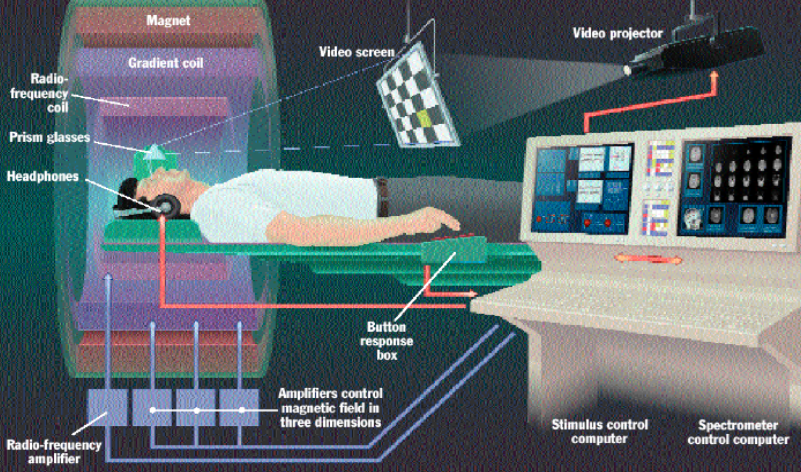
\includegraphics[scale=0.3]{fmri.png}
\end{center}
\caption{An fMRI experiment}
\label{fig:fmri}
\end{figure}

For example, below displays an image viewed by a subject in the fMRI machine and a reconstruction of their brain activity at that moment. The blue regions of the brain shows regions of low activity in the brain and the red regions correspond to high activity \textcolor{red}{(is this right?)}.

\begin{figure}[H]
\begin{center}
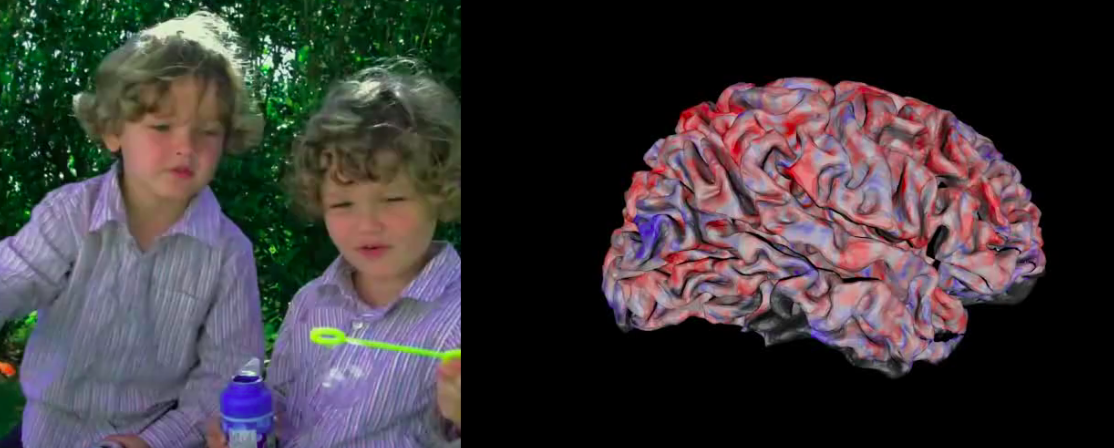
\includegraphics[scale=0.2]{brain.png}
\end{center}
\caption{The brain's response to viewings of an image}
\label{fig:fmri}
\end{figure}


Amazingly, we were able to use fMRI data to reconstruct short segments of film trailers shown to the subjects as the video below shows. There were 7200 seconds of training videos and 5400 seconds of test videos. Some people call this ``mind-reading'' although really it's just data visualization and prediction. \textcolor{red}{give more details of how we did this. It wasn't clear to me from the lecture...}


\subsection*{Predicting brain activity in the visual cortex: The Gallant Lab}

Another project related to that of the fMRI movie reconstruction is the prediction of the brain's responses to visual images as measured in 20 voxels. Recall that fMRI records measurements for discretized 3D volumes of the brain (cube-like regions called voxels), much like an image can be spatially discretized into units of pixels.

For this experiment, the subject is shown pictures of everyday objects, such as a baby, or a house etc. Each picture is a $128 \times 128$ pixel gray scale image, which can be represented by a vector of length $128^2 = 16384$. These image vectors can be reduced to length $10921$ though a transformation based on Gabor wavelets.

Although the actual fMRI response to a given stimulus/image is a function of time, the response of each voxel to each image has been reduced to a single number. The question we are interested in answering using this data is ``do these features/predictors drive the brain signals?''. Once again, we seek a causal relationship.


Given that we have for each voxel response, $10921$ possible predictors from each image, we used the Lasso estimate together with cross-validation (both of which will be discussed later in the book) to identify the most important predictors. That is, for each of the 20 voxels, we are fitting a separate linear model where most of the variable coefficients have been shrunk to zero.

\begin{figure}[H]
\begin{center}
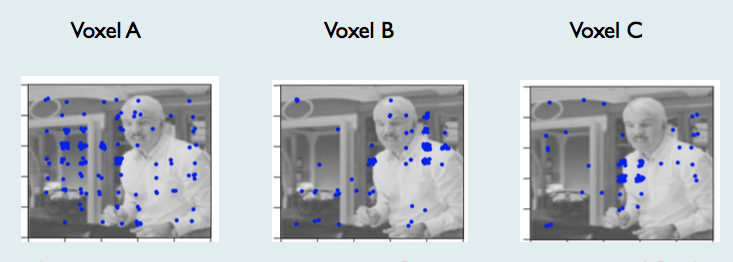
\includegraphics[scale=0.5]{voxel.png}
\end{center}
\caption{The areas within a particular image that are most useful for predicting brain activity}
\label{fig:image}
\end{figure}


For example, in the image above, the blue spots in the left-most correspond to the transformed pixels which are most important for predicting the response for voxel A, and similalry for the responses for Voxels B and C in the two subsequent images.

We could simply accept the variables that the lasso did not shrink, but wouldn't it make sense to actually look at the models being selected over each cross-validation fold?

\begin{figure}[H]
\begin{center}
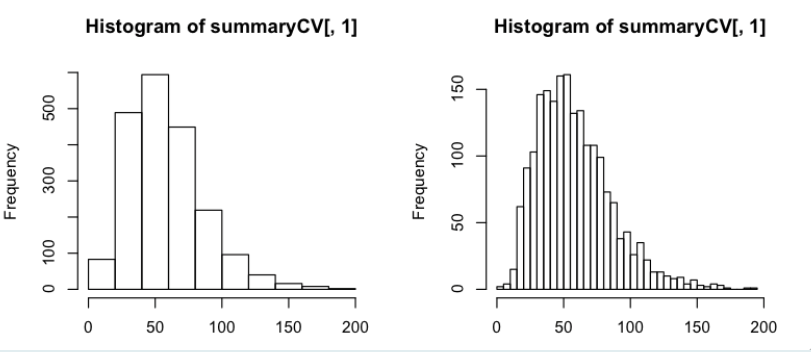
\includegraphics[scale=0.4]{voxelhist.png}
\end{center}
\caption{A histogram of the number of Gabor wavelet features selected by each model}
\label{fig:voxelhist}
\end{figure}

The figure above shows two version of the same histogram describing the number of features selected by each model. It is clear that most of the models select approximately 50 features (by shrinking all other coefficients to 0). The histogram provides us with an overview (by combining all voxels into the same plot) of the models that we have fitted to this data. What have we assumed by visualizing all voxels simultaneously? Primarily, we are assuming that the voxels are comparable to one another, an assumption that seems reasonable. However, it would probably be a good idea to look at the voxels individually as well, since with this combined approach, we might be masking some interesting information corresponding to individual voxels. 

\subsubsection{Assumptions}

It is probably not a reasonable assumption that the voxels are independent to one another, right? But as soon as we don't have independence, some of the most useful models are no longer applicable. Often we assume independence because we don't know how to model the dependence. Most assumptions that we make on our data are assumptions of convenience. Thus the question becomes, if the assumptions of our model are a little bit wrong, how much of an impact will this have on our conclusions drawn from these models? 


Further, what assumptions would we be making by combining the voxel responses from different people? We collected the voxel responses from a number of people, but we chose to analyze them separately. Why? The primary reason is that to combine the data from different people would mean that we had to ensure that the data were normalized (and thus comparable). But how could we do this? In a lot of applied problems, people simply collate their data from different sources together without considering whether this action makes sense.

The issue of normalization is also extremely prevelent in areas of bioinformatics, whereby each run of an experiment has different sources of bias. When the microarray technology first appeared, it was the first time scientists were able to actually look at the expression levels of multiple genes at once. The process of microarray data generation is very physical; someone must fluorescently tag the genes with chemicals and wash away the genetic materials that are not of interest. The data requires so much pre-processing and can be so noisy. \textcolor{red}{Perhaps talk about normalization in terms of microarray data more}. 

It is also common to center the data to have mean zero and standardize so that all observations have standard deviation 1. 







\section{Cloud detection over polar regions}

This project focuses on predicting the presence of clouds in polar regions, which is notable difficult due to the resemblance of clouds to snow from satellite images. Cloud coverage is a key feature of predictive climate models due to the cloud's ability to both act as a blanket to trap heat in the lower atmosphere as well as their ability to reflect rays from the outer atmosphere. Uncertainties about the impact of cloud radiation feedback on the global climate are among the greatest obstacles in understanding and predicting the future of Earth's climate, however the presence of cloud above snow and ice covered surfaces is particularly difficult to detect from satellite images due to the similar reflective and temporal properties of cloud and snow. 

In the late 1990s, NASA launched a satellite called Terra as a part of NASA’s Earth Observing System (EOS), the goal of which is to improve the scientific understanding of global climate changes and provide the scientific basis for environmental policies. Terra was equipped with instruments including a Multi-angle Imaging SpectroRadiometer (MISR), a camera that is used to take pictures of the earth below from multiple angles. NASA's goal for this satellite was to capture images of the Earth each from multiple angles in order to increase understanding of the Earth's systems. At each location, an image is taken from 9 different angles, resulting in images of 9 separate locations. However, as the satellite moves along its path, images of each location are taken from all subsequent angles (see the figure below). Further, each of these images is recorded using 4 different (443nm, 555nm, 670nm, and 865nm Near Infrared Red) wavelengths at each angle.

\begin{figure}[H]
\begin{center}
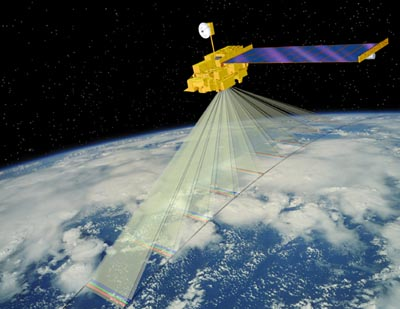
\includegraphics[scale=0.4]{misr.jpg}
\end{center}
\caption{The MISR camera}
\label{fig:misr}
\end{figure}


The MISR algorithm retrieves the cloud height and cloud movement by matching the same cloud in images obtained from three different angles. This algorithm works very well when detecting clouds over darker surfaces such as deep ocean or vegetation covered land surface, but is less effective over snow and ice covered surfaces due to the difficulty in matching.

\begin{figure}[H]
\begin{center}
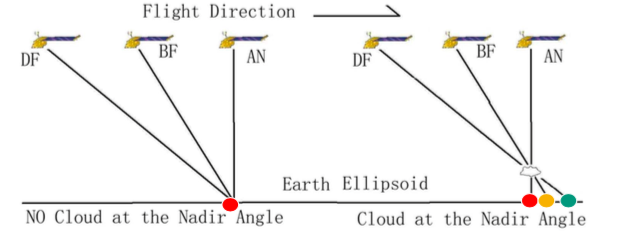
\includegraphics[scale=0.4]{misr_detect.png}
\end{center}
\caption{The MISR camera}
\label{fig:misr2}
\end{figure}

Consider, for example, the figures presented blow. The top panel in the figure below shows a situation in which cloud is easy to detect as it cloud appears over a deep body of water, whereas the second panel displays clouds appearing over ice/snow in Greenland.


\begin{figure}[H]
\begin{center}
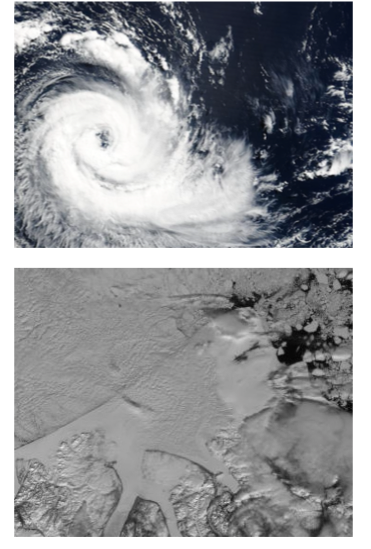
\includegraphics[scale=0.4]{cloud.png}
\end{center}
\caption{Different clouds}
\label{fig:clouds}
\end{figure}



\subsection*{Inital approaches to cloud detection in polar regions: LCMC}

An initial approach (Shi et al. 2002), LCMC, utilizes the domain knowledge that correlations between angles are high over snow and ice covered regions but weak for regions covered by high clouds. Further, clouds are brigher than snow and ice covered surfaces in forward angles (see the figures below). 

\begin{figure}[H]
\begin{center}
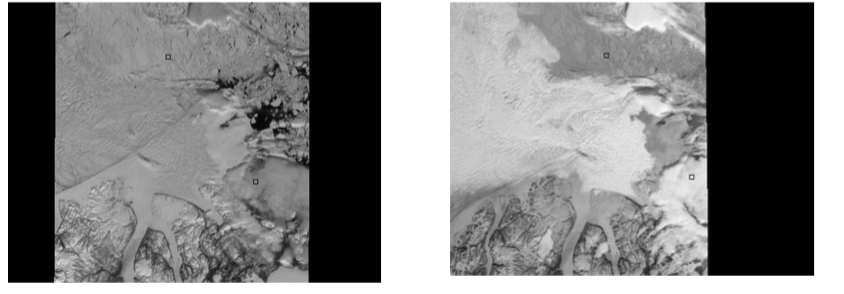
\includegraphics[scale=0.4]{cloud_angles.png}
\end{center}
\caption{Images of clouds over ice regions taken from different angles. The left panel corresponds to the image taken from the AN angle and the right panel corresponds to the image taken from the DF angle}
\label{fig:clouds}
\end{figure}


To utilize this information, this approaches focuses on identifying regions of snow or ice rather than clouds. However, this approach fails in regions where the surface is smooth (such as frozen rivers) or there are thin clouds. How could we adapt the method to rectify these issues? We could use SD to measure smoothness and forward scattering via DF to deal with thin clouds \textcolor{red}{what?}

\subsection*{The Enhanced LCMC algorithm}

The enhanced LCMC algorithn (ELCMC) thresholds 3 features based on 275m, terrain projected red radiances. Instead of utilizing the expert labels, this approach performs clustering (an example of unsupervised learning). The three features are

\begin{enumerate}
\item The correlation between different angles measured by 
$$CORR = \frac{r_{AF - AN} + r_{BF - AN}}{2}$$
\item Surface smoothness measured by $SD_{AN}$
\item The angular signature of the radiances from different angles: Normalized Difference Angular Index (NDAI) see Nolin, Fetterer, and Scambos (2002), measured by
$$NDAI = \frac{Radiance_{DF} - Radiance_{AN}}{Radiance_{DF} + Radiance_{AN}}$$
\end{enumerate}

The algorithm works be predicting that a pixel is clear of cloud (contains snow and/or ice) when our values satisfy at least one of two thresholding criteria:

$$SD_{AN} < threshold_{sd}$$

or when

$$ CORR > threshold_{corr} ~~~ \textrm{ and } ~~~ NDAI < theshold_{ndai}$$

where the thresholding values are either fixed or adaptively chosen. If neither of these two conditions are satisfied, then the pixel is predicted to be cloudy.


\begin{figure}[H]
\begin{center}
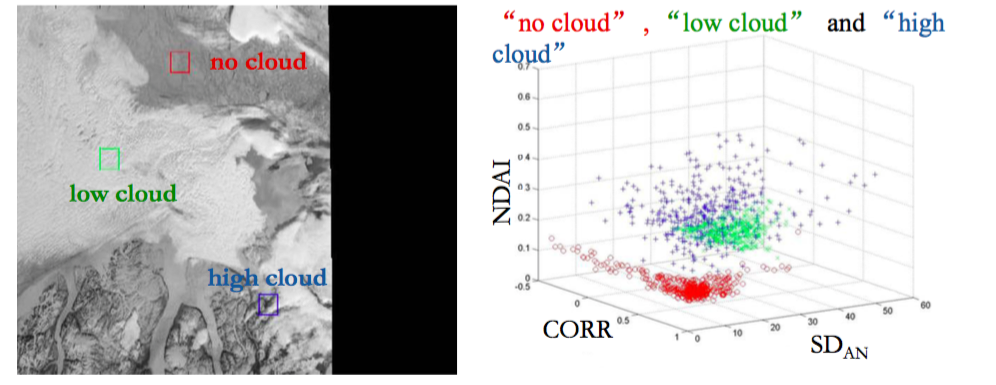
\includegraphics[scale=0.4]{ELCMC.png}
\end{center}
\caption{The ELCMC algorithm}
\label{fig:elcmc}
\end{figure}







\part{Causal Inference}



\chapter{An introduction to causal inference}
\label{ch:causal}



Have you ever heard the phrase ``correlation does not imply causation''? Chances are that you have (perhaps it was even accompanied by a humorous graph describing how the age of Miss America is correlated with the rate of murders by steam, hot vapors and hot objects), yet although everyone and their dog is capable of uttering the phrase, few appear to really understand it. It is in fact extremely common for human beings to jump to an inference of causation from an observation of correlation. It is not hard to postulate reasons for why this fallacy is so common. One could argue that the fundamental human tendency to infer causation arose as a result of our innate need to understand and explain the world in which we live, and even offers an evolutionary advantage. Our inclination to draw causal conclusions begins from a young age; for example, as a child we learn that touching a hot object causes pain. At such a young age, we don't understand the mechanism of \textit{why} we felt pain when we touched the hot object, but we inferred that it was indeed the physical act of \emph{touching} the object that \emph{caused} the pain. The end result being that we quickly learn to stop touching hot objects, no matter how appealing they seem.

Although in most every day encounters we don't have the means to explain the mechanism of cause and effect, oftentimes our intuition that lead us to infer causation from correlation is indeed correct. The problem arises when we continue to draw this need to infer causation into the complex realm of science. As an example, consider drug advertisements: most drug advertisements feature extraordinarily happy and healthy people, bright colors, accompanied by a passing description of what the drug is actually for. The idea behind these advertisements is that the human mind automatically infers causation from the association presented between the drug and the happy people. The aim is to make the viewer infer that the drug \emph{causes} health and happiness (which, if you pay attention to the hurriedly reported side-effects at the end of the ad, is likely the opposite of what the drug causes). 

\subsection*{The egg-yolk study}


\textcolor{red}{Description and discussion of study needs work!}


For a more concrete example, let's consider a Canadian study by Spence et al. on egg yolk consumption and cartoid plaque which aimed to identify whether the atherosclerosis burden (as a marker of arterial damage) was related to regular consumption of egg-yolk. The results of the study were discussed in the media using tag lines such as ``a new study suggests eating egg yolks can accelerate heart disease almost as much as smoking'', and ``No yolk: [is] eating the whole egg as dangerous as smoking?''.

The study was based on an 2831 consecutive patients attending vascular prevention clinics at University Hospital were asked to fill out a lifestyle questionnaire at the time of referral to the vascular prevention clinic. From the questionnaire, the authors calculated for each patient pack-years of smoking (number of packs per day of cigarettes times the number of years of smoking) and egg-yolk years (number of egg yolks per week times the number of years consumed). For each patient, each plaque identified in the common, external and internal carotid artery on both sides was measured in a longitudinal view, in the plane in which it was biggest. The perimeter of each plaque was measured by tracing a cursor on a computer screen. Of the 2831 patients with data on egg yolk consumption, 1231 consented to use the data and had data on pack-years of smoking and carotid total plaque area. Data range checks were performed and data entry errors such as decimal errors were identified by scatterplots of age against each continuous variable. The author's interpretation of the results in their study is that the ``data suggests a strong association between egg consumption and carotid plaque burden'', and they conclude that their ``findings suggest that regular consumption of egg yolk should be avoided by persons at risk of cardiovascular disease''.



Can you see any issues with this study? Are the conclusions drawn reasonable?


There are in fact a number of issues:

\begin{enumerate}
\item The study is only considering people who had been referred to a particular vascular prevention clinic, yet the conclusion is making claims about the general population.
\item The study is observational AND they have no control group for comparison.
\item  Do the measurements of plaque area seem reasonable? To me they seem very crude and are potentially a large source of error. This was not discussed at all in the media reports of the study.
\item ``All patients with complete data for each analysis were included'': there is no explanation of how many patients had incomplete data, nor potential reasons for this. For example, what if people who did not consume egg-yolks or smoke simply chose not to fill out the questionnaire.
\item Less than half of the original study population were actually used in the study (either as a result of lack of consent or missing data) -- we are offered no information on how those who were used in the study differ from those who were not.
\item They jumped to causation in their conclusion by suggesting that ``regular consumption of egg yolk should be avoided by persons at risk of cardiovascular disease'', which implies that consumption of egg yolk \emph{causes} heart disease.
\end{enumerate}




There is a common misconception that a study with a large sample size is automatically better than a smaller one. However a large study with a poor design will almost never be better than a smaller study with a great design. Compare the relatively large egg-yolk study with the NZ filmmaker \textcolor{red}{Name? Reference?} who put himself on a calorie controlled diet, but ensured that all of the calories came from high-fat junk food. Within 8 weeks he had gained an enormous amount of weight. This is a study with only one person (an incredibly small sample size), but which study would you believe more? 


\section{Treatment assignment mechanisms}

In the egg-yolk study described above, we discussed the many issues with the study and touched upon why it didn't provide enough evidence to draw a causal conclusion. We now move on to discuss the general principles for designing studies from which we \textit{could} conceivably draw causal conclusions. In doing so, we will introduce the Neyman-Rubin framework for causal inference.




It is generally considered that the gold-standard for drawing causal inferences is to conduct a \textbf{randomized, controlled experiment}. The idea behind this notion is as follows: suppose that, from your population of interest, you randomly select $N$ people. You then randomly split your sample in half, so that $N/2$ are in the ``treatment'' group and $N/2$ are in the ``control'' group. Then, on average, the treatment and control groups would be statistically equivalent (the covariate distributions of the two groups should be more or less the same). In particular, if we apply an intervention (a treatment) to the treatment group, but not to the control group, then the only difference between these two groups becomes the fact that the treatment group received the treatment and the control group did not. Thus any difference observed between the two groups after applying the treatment must be a caused by the treatment itself (rather than a reflection of some initial underlying difference between the two groups: if the randomization worked, there should be no underlying difference).

In contrast to the randomized experiment we just described, an \textbf{observational study} is one in which the experimenter simply observes the differences between subjects who have placed themselves in the treatment group and those who have not. In a randomized, controlled experiment the experimenter decided, albeit randomly, who received the treatment and who did not, whereas in an observational study, the experimenter has no control over the treatment assignment. What is the problem with this approach? The primary problem is that there might be underlying differences between the treatment and control groups. In this case, we can never be certain that the differences that we observe were a result of the treatment rather than some underlying difference. Even if we only compare treated individuals with control individuals whose measured \textbf{covariates} (variables related to the response) are similar, there is always the possibility that there are unobserved variables that differ between the two groups. Randomization guarantees that, on average, \textit{all} covariates (observed or unobserved) are balanced.

Suppose, for an example, that we wanted to estimate the causal effect of smoking on the incidence of cancer. The response in this example is a binary indicator of whether an individual develops lung cancer or not, and possible covariates include age, gender, race and various socio-economic variables. It would certainly be unethical to randomly assign half of our sample of people to smoke and the other half not to be. A much more reasonable approach would be to compare people who are already smokers to people who are not smokers and calculate the difference in the proportion of people in each group who develop lung cancer. What if, however, there existed underlying differences between people who chose to smoke and people who do not (for example genetic differences, which at the time, were unobservable) which caused people both to smoke and to develop lung cancer. In this case, smoking doesn't cause lung cancer at all. In fact, this was the argument used by many tobacco companies to dispute the many observational studies that began to arise claiming that smoking caused lung cancer.

As mentioned, the principal problem with observational studies is that there may be underlying differences between the treatment and control group, other than the treatment itself, which influences the response. Such variables are called \textbf{confounders}. The question to ask of observational studies thus becomes: how can we be sure that any differences we observe between the treatment and the control groups are due to the treatment rather than confounding variables?




\subsection*{Inferring causation from randomized studies}

The most obvious arguments for conducting randomized studies are related to the issues discussed above to encourage balanced covariates between the treatment and control groups. However, there is a common misconception that randomization \emph{ensures} balanced covariates. This is not necessarily true, and the likelihood of balanced covariates depends strongly on the randomization procedure undertaken. Consider, for example, the case where assignment to treatment is done by the flip of a coin: for each individual, if the coin flip shows heads then they are assigned to the treatment group, and if it shows tails they are assigned to the control group. Then, in a study with $N$ individuals, there are $2^N$ different possible ways to treatment assignment (each individual has two possible assignments: treatment or control). Moreover, several of these treatment assignment outcomes result in useless studies: it is entirely possible (though unlikely) that under this randomization procedure, everyone will be assigned to the treatment group. In which case it is impossible to make a causal inference about the effect of the treatment on the response (since you have no control group to compare to).

For another example, consider a study aimed at assessing the effectiveness of a type of heart surgery on 1,000 patients from a total of 12 different hospitals. Surely the outcome will vary from hospital to hospital. Thus even if the randomization is conducted such that half of the patients are in the treatment group and the other half are in the control group, there is the possibility that the treatment group will contain only patients from hospitals 1, 2, 4, 7, 8 and 12 and the control group contained only patients from hospitals 3, 5, 6, 9, 10 and 11. This mechanism has the property that we are never comparing patients from the same hospital, moreover, it is likely that each hospital is different, and thus that our treatment and control groups are not necessarily comparable. How could we conduct the randomization to increase the chance obtaining more comparable (more balanced) treatment and control groups? One way is to perform the randomization procedure individually \emph{within} each hospital. This process is called \emph{stratification}.

Thus it is certainly not the case that a randomization ensures that the study will be well-designed, but hopefully we can agree that randomization studies are more likely to lead to balanced covariates than observational studies. An analyst needs to think carefully about how to conduct the randomization to ensure that the control and treatment groups are equivalent. In the (rare) case that the covariates are perfectly balanced between the treatment and control groups, then to obtain an unbiased estimate the causal effect of the treatment, we could simply calculate:

$$(\textrm{Average outcome of the treatment group}) - (\textrm{Average outcome of the control group})$$

In ideal situations, this is the only number we ever really need to look at. Why would we need to fit linear models or conduct hypothesis tests when the difference in average outcomes tells us everything we need to know. \textcolor{red}{Expand on this}

Another point in favor of randomization of treatment assignment is that it makes the randomness in the problem explicit. More specifically, we know exactly how the randomness was created and it is easily replicable. As we will discuss when we introduce the Neyman-Rubin causal inference model, the only randomness in these types of problems comes from the assignment to treatment (in particular, the measured outcome is non-random). This is strikingly different to the traditional approach in which the outcome of interest is a random variable and the traditional approaches such as hypothesis testing and confidence intervals rest on properly defined probability distributions or sample spaces. This allows for more transparency in the problem.


Randomization is certainly the gold-standard in inferring causation (although it is important not to accept a study as perfect just because the experiment was randomized. See the fruitfly experiment as an example).

Although the first people to truly emphasize the importance of randomization was R.A Fisher did so for experimental reasons. \textcolor{red}{a history of randomization}. These days, randomization has many uses beyond just experimental design. The modern approaches involve many randomized algorithms such as: compressed sensing, randomized algorithms for big data, Shannon's randomized channel code, random projections, non-parametric testing, etc.


\subsection*{Inferring causation from observational studies}

As discussed above, using randomized experiments it's certainly possible to infer that a treatment \emph{causes} a change in some outcome, however we haven't yet discussed whether it's even possible to infer causation from observational studies. You may have heard the phrase \emph{``no causation without manipulation''}, however we will consider an example (smoking) that represents a counterexample.


\begin{itemize}
\item matching - consider all confounders (never know if you've observed \emph{all} of them!)
\item
\end{itemize}



This is great news -- there are certainly many instances in which observational trials would be preferred to randomized trials.

\section{The Neyman-Rubin model}

Everything we have discussed in this chapter so far has a philosophical and non-rigorous flavor to it. The Neyman-Rubin framework allows us to introduce rigor into the vague language of causal inference. The Neyman-Rubin model is named after Jerzy Neyman, who introduced the potential-outcomes framework for causality in 1923, and Donald Rubin who is a pioneer in extending this framework into the modern of causal inference in observational and randomized experiments.

The model is rooted in the notion that each individual in a two-arm study (control and treatment) has two \emph{potential outcomes}. To make our descriptions transparent, we will embed our description of the Neyman-Rubin model within an example: suppose that we are interested in testing the effectiveness of a new drug on reducing the incidence of monthly headaches (our response). The patients assigned to the control group are not provided with the drug (perhaps they are provided with a placebo to make the study blinded, but we won't worry about this now), while the patients in the treatment group are provided with the drug and are told to take it daily. Each patient in each group then reports the number of headaches they experience in a month.

Let's think hypothetically about an individual patient (patient $i$). Suppose that when patient $i$ is assigned to the control group, they report experiencing 10 headaches. The notation we use is $Y_{i0} = 10$, where the 0 index corresponds to ``control''. Alternatively, when patient $i$ is assigned to the treatment group, they report experiencing 8 headaches, and we write $Y_{i1} = 8$, where the 1 index corresponds to ``treatment''. In reality, however, we can \emph{only observe one} of these outcomes, since patient $i$ will be assigned \emph{either} to the control group or to the treatment group, \emph{but not both}. Hence we call $Y_{i0}$ and $Y_{i1}$ the \emph{potential outcomes} for patient $i$. It is crucial to realize that both $Y_{i0}$ and $Y_{i1}$ are \emph{fixed} values (i.e. they are not random!). The \emph{observed} outcome (the outcome that we actually observe) for patient $i$ can be written as

$$Y_i = (1 - T_i) Y_{i0} + T_i Y_{i1}$$

where $T_i = 1$ if patient $i$ is assigned to the treatment group and $T_i = 0$ if patient $i$ is assigned to the control (recall that only one of these will occur). Note that if patient $i$ is assigned to the treatment group, we have

$$Y_i = 0 \times Y_{i0} + 1 \times Y_{i1} = Y_{i1}$$

whereas if patient $i$ is assigned to the control group, we have

$$Y_i = 1 \times Y_{i0} + 0 \times Y_{i1} = Y_{i0}$$

That is, we observe the potential outcome corresponding to which group patient $i$ is assigned.


\subsubsection*{Randomness in the Neyman-Rubin model}

When presented with a new formulation or model, it is good practice to ask ``where does the randomness come from in this model?''. In essence, we are asking ``what assumptions are we making about the randomness by using this model?''.

Recall that the potential outcomes, $Y_{i0}$ and $Y_{i1}$, are considered \emph{fixed} (non-random) values. The observed outcome, $Y_i$, however, is considered to be random. But given that $Y_i$ is just a linear combination of the potential outcomes, where does the randomness come from? The answer is that the randomness comes from the treatment assignment variable, $T_i$. That is, under this formulation, the only reason that we consider the observed outcome to be random is because the decision to place the patient in the treatment group or control group was random.


Thus the key difference between the Neyman-Rubin formulation and the traditional formulation is that in the Neyman-Rubin formulation a subject's outcome under each treatment is considered fixed, but the outcome that we observe is random (since it is random which treatment group the subject will be assigned to). In the traditional formulation, the response is considered to be random itself, but it is usually not explained where the randomness comes from. That is, the Neyman-Rubin model makes the randomness explicit!

\textcolor{red}{I need to explain what I mean by the ``traditional formulation''}

Note that in the typical setting, we consider the randomness to come from the sampling procedure where we draw our sample from the population. Although this randomness also exists when we use the Neyman-Rubin model, we are not using this source of randomness for our analysis. In the Neyman-Rubin model, the primary source of randomness comes from the random assignment to the treatment or control group.

\subsection*{Estimating the causal effect: an example}


Let's consider an example: suppose that you were the inventor of a new painkiller, and you needed to prove to the FDA that the painkiller was effective. How would you do this? Ideally, you would be able to perform a randomized trial Suppose that you had access to patients who visited a certain medical clinic over a period of a year. Then for each new patient who consented to participate in the trial, and whose primary reason for visiting the clinic was pain, you could conduct a random ``coin toss'' to decide if the doctor will prescribe the new painkiller to the patient or not. Note that in general the doctor cannot decide themselves whether or not to prescribe the painkiller, since this will introduce personal selection bias into the experiment, rather, the doctor must follow the decision made by an automated ``randomized'' process at the trial center. If the doctor is instructed to assign the patient to the treatment group, then they will prescribe the patient with the new painkiller, otherwise they will prescribe the patient to follow existing pain reliving paths. Over the duration of the trial, each enrolled patient must self-report their pain level on a scale of 1 to 10 (regardless of whether or not they received the new painkiller), and send their reports to the trial center. We are interested in identifying whether or not there is a difference in average headache severity between those who received the new painkiller and those who did not. To place this in the Neyman-Rubin framework, for patient $i$, we observe the average headache severity $Y_{i}$ which will be one of the two possible potential outcomes:

$$Y_{i} = \begin{cases} Y_{i0} & \textrm{ if patient $i$ is assigned to the control group} \\ 
Y_{i1} & \text{ if patient $i$ is assigned to the treatment group} \end{cases}$$ 


That is, if patient $i$ is assigned to receive the new painkiller, we will observe the outcome $Y_{i1}$ (for example $Y_{i1} = 4$ implies that if the patient is assigned to take the new painkiller, they will have an average headache severity of 4), and we will observe the outcome $Y_{i0}$ otherwise (for example $Y_{i0} = 6$ implies that if the patient is not assigned to take the new painkiller, they will have an average headache severity of 6). Clearly we can only observe $Y_i = Y_{i0}$ or $Y_i = Y_{i1}$ based on treatment assignment. As discussed above, this can be re-written as

$$Y_i = (1 - T_i) Y_{i0} + T_i T_{i1}$$

where $T_i = 1$ if patient $i$ is assigned to the treatment group and $T_i = 0$ otherwise.


We are interested in identifying the effect of the treatment (being prescribed the placebo) on the outcome. Ideally, we would like to measure the difference between the outcome when assigned to treatment and when assigned to control for each person, i.e. we would like to observe $Y_{i1} - Y_{i0}$ (the difference in average headache intensity for patient $i$ for when they receive the painkiller and when they don't), and take the average over all patients enrolled in the study. This is called the sample average treatment effect (SATE):

$$SATE = \frac{1}{n}\sum_{i=1}^n (Y_{i1} - Y_{i0})$$

and it estimates the treatment effect (the effect of prescribing the painkiller). However, the SATE is not observable since for an individual we observe either $Y_{i1}$ OR $Y_{i0}$, not both (thus we certainly cannot calculate the difference $Y_{i1} - Y_{i0}$. An unbiased estimate of the SATE, however, can be given by the obvious estimator

$$\frac{1}{n_1} \sum_{i:T_i = 1} Y_{i} - \frac{1}{n_0} \sum_{i:T_i = 0} Y_{i}$$

whereby we are taking the average of the outcomes observed for those in the treatment group and subtracting the average of the outcomes observed for those in the control group. 



\subsection*{Hypothesis testing for treatment effect}



The notion of identifying a treatment effect can also be phrased as a hypothesis testing problem. Fisher posed this problem as testing the null hypothesis that

$$H_0: Y_{i1} = Y_{i0}$$

i.e. the treatment has \emph{no effect on anyone}. This hypothesis, however, is not something that we can directly test since, once again, for each $i$ we only observe one of $Y_{i1}$ and $Y_{i0}$, and so cannot test the hypothesis that they will be the same. Alternatively, we can test the weaker hypothesis 

$$H_0: \mu_1 = \mu_0$$

where $\mu_1$ is the population average response of those assigned to the treatment, and $\mu_0$ is the population average response of those assigned to control. This null hypothesis is equivalent to the claim that there is no difference between the average outcome of the control and the treatment groups. This hypothesis is in fact testable, and a suitable test statistic can be found in the SATE:

$$\tau = \overline{Y}_1^{obs} - \overline{Y}_0^{obs}$$

where $\overline{Y}_1^{obs} = \frac{1}{n_1} \sum_{i:T_i = 1}Y_i$ is the average outcome for the treatment group and $\overline{Y}_0^{obs} = \frac{1}{n_0} \sum_{i:T_i = 0}Y_i$ is the average outcome for the control group.

How do we obtain a notion of significance for this test statistic? Rather than estimating the variance of $\tau$, and using a distributional result to obtain a $p$-value, it is more common to conduct a permutation test to approximate the null distribution of $\tau$ and thus obtain a $p$-value. For a specific example, suppose that we had randomly assigned 500 children in 3rd grade to drink milk every day and another 500 children in 3rd grade to never drink milk. Suppose that the height difference that we observed between these two groups after a year was 2 inches. The question is, given that we have observed a difference of $\overline{Y}_T - \overline{Y}_C = 2$, how do we know that this is a ``significant'', or real, finding, not just the result of random chance?

If the treatment (drinking milk daily) truly had no effect, then we would imagine that if instead different partitions of the 1000 children into two groups of 500 had been drawn, then there we would observe a similar height difference as in the original experiment. Thus, a way of seeing whether the treatment did in fact make a difference, we would ideally like to compare this value to the height difference that we would have obtained from all other permutations of treatment assignment. To formalize this somewhat, under the \emph{strong null hypothesis} (that $Y_i(1) = Y_i(0)$ for all $i$), we can randomly flip the treatment indicator and obtain the same results. If we can show that the value of our test statistic, $\tau$, that we obtained from our original experiment is extreme (very large or very small) compared to the values obtained in situations when we have randomly permuted the treatment vector, then this implies that our sample is not a typical representation of this null situation in which there is no difference between the outcome observed under treatment and control. In this case, we typically say that our result is ``significant''.


\begin{enumerate}
\item Calculate the value of the test statistic, $\tau$
\item Randomly re-shuffle (permute) the treatment and assignment labels for each individual. For example if we had a (pathetically small) study involving 6 people, whose treatment assignments were $T = (1, 0, 0, 1, 0, 1)$ (i.e. individuals 1, 4 and 6 were assigned to treatment and individuals 2, 3 and 5 were assigned to control), we would randomly rearrange the order of the values in $T$ to get, for example, $T^* = (1, 1, 0, 1, 0, 0)$. 
\item Re-evaluate the value of $\tau$ using the treatment assignment given by $T^*$: 
$$\tau^* = \frac{1}{n_1} \sum_{i:T^*_i = 1}Y_i - \frac{1}{n_0} \sum_{i:T^*_i = 0}Y_i$$
\item Repeat steps 2 and 3 many times (this will give an empirical estimate of the null distribution of $\tau$, whereby we are assuming that treatment and control are exchangeable: under the null hypothesis the treatment has no effect)
\item Calculate a $p$-value by calculating the proportion of $\tau^*$ values that are more ``extreme'' (larger in absolute value) than our true value, $\tau$.
\end{enumerate}

\section{Notes}



In this chapter, we have just touched on the deep field of causal inference. For those who would like to delve further into the Neyman-Rubin approach to causal inference and learn more about the existing methods for conducting and analyzing experimental and observational experiments, Imbens and Rubin's book, Causal Inference for Statistics, Social, and Biomedical Sciences: An Introduction, is an excellent resource.

Further, it is worth noting that there are a number of alternative approaches to the language of causal inference, the most prominent of which is that of graphical models introduced by Judea Pearl.





\part{General topics/methods that you should know about before moving on}



\chapter{The bias-variance tradeoff}
\label{ch:tradeoff}







Throughout our data analysis adventures, it is vital to identify how various sources of error we encounter might lead to ``incorrect'' or ``unreliable'' estimates. Such knowledge would allow us to improve the models we fit by manipulating the tradeoff between bias (how close our estimate is on average to the true value) and variance (how much our estimate varies over repeated samples).

In essence, the bias-variance tradeoff captures the tradeoff between accuracy and reliability of our estimates. 



\section{Bias}

Before describing the bias-variance tradeoff, we will first delve into a discussion of bias itself. For a technical definition, the bias of an estimator $T(X)$ (where $T(X)$ is simply a statistic: a function of our data such as the sample mean $\bar{X}$) of a parameter $\theta$ is defined to be 

$$\text{Bias} = E(T(X)) - \theta$$


If $T(X)$ is an unbiased estimator of $\theta$, then $E(T(X)) = \theta$: on average (assuming we could take repeated samples from our population and recalculate our estimate), the value of our estimator is equal to the \emph{true} value of the parameter.




Suppose that we've just obtained some data $x_1, ..., x_n$, let's say the heights of $n$ randomly selected people. Suppose that we plot a histogram the $n$ data points and conclude that the histogram looks kind of Gaussian (obviously we are only observing a sample so we will never have \emph{exactly} normal data). Let's think for a moment about the assumption that the true distribution of the data is actually a normal distribution with mean $\mu$ and variance $\sigma^2$. Do you really believe that the data that you observe was exactly generated by this distribution? Probably not, right? The \textbf{true} underlying distribution of the data, in general, cannot be \emph{exactly} specified. If we assume that the data comes from a specific space of probability distributions (such as the space of normal distributions indexed by $\mu$ and $\sigma$), then the \emph{bias} of this assumption/estimation is the ``distance'' (in some sense) between the distribution that we assumed and the ``true'' distribution. An example of the distance between the true (unknown) distribution, $P^*$, and our assumed distribution, $P_\theta$, is the Kullback-Leibler divergence (a distance metric very prominent in information theory):

$$D_{KL}(P^* \vert \vert P_\theta) = \int_{-\infty}^\infty p^*(x) \ln \frac{p^*(x)}{p_{\theta}(x)} dx$$

where $p^*$ and $p_\theta$ denote the densities of $P^*$ and $P_\theta$. It is not hard to see that minimizing this quantity is actually the same as finding the $\theta$ that maximizes likelihood:

$$
\begin{aligned}
D_{KL}(P^* \vert \vert P_\theta) & = \int p^*(x) \ln p^*(x) dx - \int p^*(x) \ln p_\theta(x) dx\\
& = - H\left(p^*(x)\right) - \int p^*(x) \ln p_\theta(x) dx\\
& = - H\left(p^*(x)\right) - E\left(\ln p_\theta(x) \right)
\end{aligned}
$$

Where $H\left(p^*(x)\right)$ is something called the \emph{entropy} of $p^*(x)$, which is independent of $\theta$. Thus, if we want to find the best $P_{\theta}$, we want to minimize the KL-divergence with respect to $\theta$, which is equivalent to maximizing the expected log-likelihood, $E(\ln p_\theta(x))$ (or minimizing the negative expected log-likelihood).



Thus it is important to be aware that the parametric bias that we see in text books essentially assumes that the distribution we assume is the true distribution. It is important to think about the context! 



Most of the statistical literature lives within the world that assumes specific distributions in asymptotic settings. However, in reality, we will never truly be able to reach the land of asymptotics. Thus, when applying theoretical results to real data, it is important to take the conclusions with a grain of salt: the assumptions behind the results are almost never more than approximately satisfied. The mathematics are only relevant when your approximation is good enough relative to the precision you're looking for. We should worry about how accurate the assumptions we're making are, and if they are not valid, how does this affect the conclusions we draw?

In fact, talking about the existence of an underlying truth in any setting is already a fairly hefty assumption. 




Where does bias come from? Bias can arise from various sources, such as our sampling procedure (if we are interested in estimating the average height of members of a population, but we accidentally sample many more men than women, then we are getting an upward biased estimate of height for the entire population), as well as the model (estimator) we use.

\section{Variance}

Suppose that we were interested in measuring the average height of all students enrolled at UC Berkeley (this is our population of interest). Assuming that we have only one hour to do so, we cannot possibly measure the height of every enrolled student, since many will not be at the campus during that hour. Thus we must suffice to estimate the average height of all students using a random sample of students drawn from those on campus during the given hour. From this sample of students, we calculate their average height, and assuming that this sample of students can be thought of as ``randomly selected'' from the overall student population, this height estimate will be an unbiased estimate of the average height of the entire student population. However, we have only observed a single number (the average height of all students on campus during the hour). How can we get a sense of how much this estimate would change for a different sample of students? 

It is important to realize that this estimate of average height is in fact a \emph{random variable}. But what is random about it? Where did the randomness come from? The randomness came from the sampling procedure. We drew a random sample of the students on campus during the hour of interest, and in turn our estimate of the average height of the student population is a random number: it would have a different value for a different sample. The question is, how different might the average height be for another random sample? This question encapsulates the idea of variability. How much would our estimate vary from the mean value if we drew other samples from the population? Notationally, we typically write the variance of a random variable $X$ as

$$\text{Var}(X) = E \left( X - E(X) \right)^2$$


This entity represents, on average, how much a random variable deviates from its mean. Note that if we were considering the variance of an estimator, then the variance of the estimator describes, on average, how much the estimator (a random variable) deviates from its mean \emph{not} how much it deviates from the ``true'' value of the parameter (unless the estimator is unbiased).

If we have a sample of independent and identically distributed (IID) random variables, $X = (X_1, ..., X_n)$ (this could be a sample of estimates, rather than a sample of observations), then we can estimate the true variance of $X$ by the sample variance given by

$$\widehat{\text{Var}(X)} = \frac{1}{n-1} \sum_{i=1}^n (X_i - \bar{X})^2$$

where we divide by $n-1$, rather than $n$, so that this estimator of the variance is unbiased. This result is shown in the Appendix, but you're encouraged to show that this is an unbiased estimator for the true variance of the population.


If we're willing to assume that the data comes from a normal distribution (which, for height is probably not a terrible assumption), then there exist asymptotic results that tell us the variance of our estimate when our sample size is extremely large. However, what if we didn't feel comfortable assuming normality? We could use bootstrapping (of which there exist several versions)....



When we estimate features of the population (such as model parameters) using our observed data, we are observing



\section{Question}

\begin{itemize} 
\item Describe situations where the asymptotic where the asymptotic bias and variance approximations are relevant to data analysis, as well as situations where they are not. How might we find out if the asymptotic results are relevant to the problem at hand?
\end{itemize}


\section{Manipulating the tradeoff: regularization}



We mentioned above that short bandwidths correspond to an estimator, $\hat{f}_{n, h}(x)$, of $f$ that has low bias, but high variance, whereas long bandwidths corresponds to an estimator that has high bias but low variance. Is one of these two extremes better than the other? Is it possible to obtain a happy mid-ground between the two? This is where the bias/variance trade-off comes in: perhaps we would rather find an estimator that minimizes a combination of the bias and the variance, such as the mean squared error (MSE):

$$\text{MSE} = \text{Bias}^2 + \text{Variance}$$

In fact, in modern statistics, gains are often obtained by increasing bias, but reducing variance. We can add a regularization (or smoothing) parameter to control the trade-off between bias and variance (we will return to this concept when we discuss the lasso linear model).





\section{Appendix: the sample variance is unbiased}

We want to first show that the sample variance discussed above is unbiased. Suppose that we draw an IID sample $X_1, ..., X_n$ from a population which has a true variance $\sigma^2$ and true mean $\mu$. Suppose that the values that we observe are given by $x_1, ..., x_n$ (once we actually observe the values, they are no longer random; they aren't going to suddenly change when we blink! Rather, they are rather realizations of a quantity that was generated by a random process). 

We want to show that
$$\sigma^2 = E(\widehat{\text{Var}(X)}) = E\left( \frac{1}{n-1} \sum_{i=1}^n (X_i - \bar{X})^2\right)$$

By the linearity of expectation, we have that

\begin{align*}
E(\widehat{\text{Var}(X)}) & = \frac{1}{n-1} \sum_{i=1}^n E \left( X_i - \bar{X} \right)^2\\
& =  \frac{1}{n-1} \sum_{i=1}^n E\left( X_i^2 - 2 \bar{X} X_i + \bar{X}^2 \right)\\
& = \frac{1}{n-1} \sum_{i=1}^n E\left(X_i^2 \right) - 2 E\left(\bar{X} X_i \right) + E\left( \bar{X}^2 \right)\\
& = \frac{1}{n-1} \left[\sum_{i=1}^n E\left(X_i^2 \right) - 2 n E\left(\bar{X}^2 \right) + nE\left( \bar{X}^2 \right)\right]\\
& = \frac{1}{n-1} \left[\sum_{i=1}^n E\left(X_i^2 \right) - nE\left( \bar{X}^2 \right)\right]\\
\end{align*}


Now, since we can write the variance of $X$ with variance $\sigma^2$ and mean $\mu$ (in which case the variance of $\bar{X} = \frac{\sigma^2}{n}$) as 
$$\sigma^2 = \text{Var}(X) = E\left(X_i^2\right) - \left( E\left( X_i\right)\right)^2 =  E\left(X_i^2\right)  - \mu^2$$

we have that


\begin{align*}
E(\widehat{\text{Var}(X)}) & = \frac{1}{n-1} \left[\sum_{i=1}^n (\sigma^2 + \mu^2) -  n \left(\frac{\sigma^2}{n} + \mu^2 \right) \right]\\
& = \frac{1}{n-1} \left[ n(\sigma^2 + \mu^2) -  n \left(\frac{\sigma^2}{n} + \mu^2 \right) \right]\\
& = \frac{1}{n-1} \left[ (n-1)\sigma^2 \right]\\
& = \sigma^2
\end{align*}


Thus, the given sample variance given above is an unbiased estimate for the population variance, $\sigma^2$.




\section{Answers to questions}


\begin{itemize}
\item \textbf{Describe situations where the asymptotic where the asymptotic bias and variance approximations are relevant to data analysis, as well as situations where they are not. How might we find out if the asymptotic results are relevant to the problem at hand?}\\
One example is when the model approximation error dominates the sampling error: if the class of models that you're trying to fit is extremely far from the truth, then the asymptotic results for the model become meaningless.\\
This is actually an important question to keep in mind when applying such results: when does it apply? Does my data satisfy the assumptions that make the results valid? You need evidence (although, in reality there are many assumptions that are sadly untestable)
\end{itemize}






\chapter{Hypothesis testing}
\label{ch:testing}







Talk about the Neyman-Pearson paper from lecture 5.

At the conceptual level (perhaps less so at the technical level), Neyman's point is still extremely relevant today. People still take the convenient alternative (even if it is mis-specified). It is common today to use permutation methods to perform hypothesis testing, without specifying a specific null or alternative hypothesis: such methods simply involve permuting the data and seeing if we observe something different to what we observed in the unpermuted dataset. It's not always possible to articulate an exact hypothesis. An issue with many hypothesis testing procedures and multiple hypothesis testing techniques is that they are based upon assumptions of normality.

\section{Significance}

Much of hypothesis testing is concerned with showing ``significance'', however, there is a disturbing ambiguity about what that actually means. Typically people rush to perform t-tests and claim significance if their p-value is less than 0.05, without really thinking about important things such as (1) whether a t-test is even valid and (2) what a p-value of 0.05 actually means. 


%
%Suppose, for example, that we are interested in assessing the causal effect of a treatment on some outcome of interest $y$. Recall from our discussion on [causal inference](http://rlbarter.github.io/Stat_Models_Book/3-causal.html) that such a situation can be described by the Neyman-Rubin potential outcomes framework, whereby each individual will exhibit one of two possible (fixed) responses, the response if they recieve the treatment, $Y_i(1)$, and the response if they do not, $Y_i(0)$. Then, we are interested in estimating the sample treatment effect
%
%$$\frac{1}{n} \sum_{i=1}^n Y_i(1) - Y_i(0),$$
%
%which is unobservable, since we can only ever observe one of $Y_i(1)$ and $Y_i(0)$. The treatment effect is thus often estimated by
%
%$$\frac{1}{n_1} \sum_{i: T_i = 1} Y_i - \frac{1}{n_0} \sum_{i: T_i = 0} Y_i  = \overline{Y}_T - \overline{Y}_C$$
%
%where $T_i = 1$ if observation $i$ is in the treatment group and $T_i = 0$ if observation $i$ is in the control group. Moreover, the observed outcome is defined by $Y_i = T_i Y_i(1) - (1 - T_i)Y_i(0)$.
%
%


\textcolor{red}{Come back to this section...}


\section{Normal assumptions}

When we don't have normal data (as is typically the case), we typically use the central limit theorem to justify using a t-test. The central limit theorem tells us that is we have $n$ independent and identically distributed (IID) samples $X_1, ..., X_n$ (where each $X_i$ has expected value $\mu$ and standard deviation $\sigma$), then distribution of the mean (or average), $\bar{X}_n = \frac{1}{n} \sum_{i=1}^n X_i$, tends to the normal distribution as our sample size, $n$ increases to infinity. $$\bar{X}_n  \overset{\text{approx}}{\sim} N\left(\mu, \frac{\sigma^2}{n}\right) ~~~~~~ \text{ for large $n$}$$

However, if we do not know the true standard deviation, $\sigma$, of our samples, then we have the related result that the distribution of the mean tends to a $t$ distribution with $n-1$ degrees of freedom. $$\frac{\bar{X}_n - \mu}{SE(\bar{X})} \overset{\text{approx}}{\sim} t_{n-1} ~~~~~~ \text{ for large $n$}$$


However, the approximations mentioned above are exactly that: they are \emph{approximations}. In particular, how do we know that these approximations have kicked in? If we have a non-normal, heavy tailed distribution, then the normal approximation may not kick in for small sample sizes. This might be the best that we can do in a theoretical sense, but the invention of a vast array of computational tools have allowed us to develop methods such as bootstrapping and
permutation, which have significantly fewer assumptions, and are much closer to the origins of the problems at hand.


You should really be aware when you're using normal approximations. The central limit theorem is a \emph{weak convergence}, the theorem says that it converges but doesn't say anything about how quickly it converges. But when we use it, we need our assumptions to kick in quickly, there is no use in using methods whose assumptions are satisfied only in a lovely, but mythical, place called Asymptiopia.

Only recently, people are starting to worry about using normal assumptions in maximum likelihood estimation.

In summary: these classical approaches can still be useful, but we need to worry about

\textcolor{red}{this section wasn't entirely clear from the audio -- come back
to it later...}


\section{Issues with p-values}

There is an asymmetry in terms of the null and alternative hypothesis. When we ``accept'' the null, that doesn't mean that we have \emph{proved} the null! In fact, in most cases, we need to have quite a large departure from the null in order to reject it.




\chapter{Cross-validation}
\label{ch:cv}


Cross validation (CV) is an extremely useful technique initially developed for use in model validation, but with extremely broad uses. CV is a generalization of the idea of witholding a test set from analysis for the purpose of validating results using independent data. The idea is, after we've fit a model, it would be really nice if we could test it on new data. Let's consider an example of using CV to assess prediction performance.

\begin{itemize}
\item Divide the samples into $K$ equal (or as equal as possible) cross-validation folds (subsets of the data) at random.
\item For each fold, $k = 1, 2, ..., K$, the set of observations in the $k$th fold is called the \emph{test set}, while the remaining data is called the \emph{training set}.
\begin{itemize}
\item Perform the analysis or fit the model using only the observations in the training set.
\item  Validate the analysis or assess the model fit (e.g. by calcualting prediction error) using the observations from the witheld test set.
\end{itemize}
\item Calculate the average or sum of the values calculated (such as the prediction errors) over each test set fold.
\end{itemize}





This procedure provides the user with an empirical estimate of their prediction error.



One problem with the use of cross-validation is that it is often misinterpreted as the \emph{true} prediction error. In fact, in most situations, we can never know the true prediction error (if we could, then why would we need to estimate it using cross-validation?).


As a general rule of thumb, instead of relying on cross-validation with the data you've used to define your models and to perform your analysis (although this is a reasonable thing to do, particularly for medium-sized datasets), as soon as you receive the data, you should immediately put some subset aside and not touch it until you've truly finished with your analysis. This subset will be your validation set.


As another thing to keep in mind, in general, we have no reliable way to put ``error bars'' on prediction errors generated by cross-validation.

Cross-validation can have huge error.... \textcolor{red}{show evidence}




\chapter{Normalization}
\label{ch:normalization}



There seems to be a lot of ambiguity when it comes to data normalization. First of all, what what do we mean when we say normalization? There are actually many different types of normalization! For example, there are often no clear answers given to questions such as when should I normalize my data? Should I combine data from different sources? Do I need to transform my data? We present here some guidelines for such situations, but stress that the reason such ambiguity exists, is because the answer usually comes down to making a judgment call. For example, you need to weigh up the options in terms of asking what assumptions are being made or being violated by normalizing the data.

\section{Normalization by standardization}

First of all, let's discuss the different types of normalization. Many people would think of standardization; whereby we subtract the mean and divide by the standard deviation to obtain data with mean zero and a standard deviation of 1. But even standardization raises questions: for example, what are we subtracting the mean of? Do we simply take the mean of all of the numbers in our dataset, and subtract this global mean from each number? Do do this process for each variable separately, so that each variable has zero mean and unit variance? Why not for each observation instead? Further, what if we had split our data into a training and test set; do we standardize these datasets separately after the split or together, before the split?


\section{Normalization for comparison}

There are also other kinds of normalization. For example, normalization of data from different sources to improve comparability. For example, suppose we obtained fMRI data from 10 different people. Are the responses from each person comparable? Why or why not? The data from different people may not be comparable for many reasons: for example, each run of the fMRI experiment may have slightly different calibration, each persons brain has slightly different shapes and must be transformed differently to fit the image template. 

\section{Normalization by transformation}

Perhaps instead it is a transformation that comes to mind. Some may interpret normalization to be a process that makes the data look more normally distributed, perhaps by taking the log of a variable. Recall that many theoretical results rest on the assumption that the data is normally distributed. Thus perhaps we can attempt to reduce the amount by which we violate such assumptions by making our data appear more Gaussian. When might a log-transform work well? 

\begin{enumerate}
\item If we have fit a linear model to some response which is actually multiplicatively related to the predictors, then obviously the model is not going to be an accurate representation of the relationships between the variables. Taking a log-transformation of the response however, means that we can capture this relationship using an additive linear model since if $y = a \times b$ then $\log y = \log a + \log b$. 
\item If we are using a procedure that assumes Gaussianity (which, by the way, a standard linear model does not!), and we have a skewed distribution, then taking a log-transform can downplay the skewness generating a more normal distribution:
\end{enumerate}


%http://www.geo.mtu.edu/volcanoes/vc_web/background/graphics/log.jpg
\begin{figure}[H]
\begin{center}
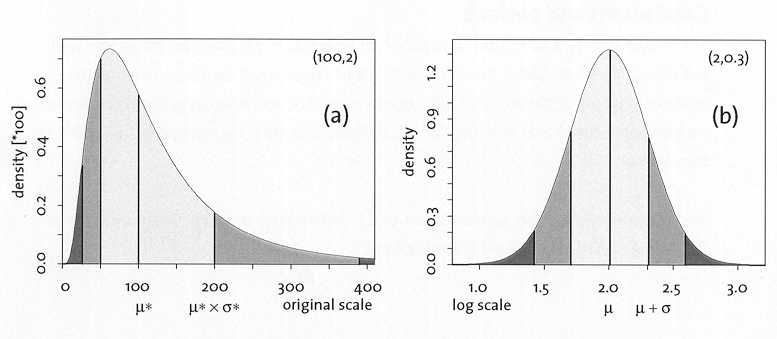
\includegraphics[scale=0.7]{log.jpg}
\end{center}
\caption{A log-transformation of a skewed distribution.}
\label{fig:log}
\end{figure}


What about other transformations? Another popular transformation is the square-root transformation. The square-root transformation is also commonly used to make data closer approximate a normal distribution. Both the log and the square-root transformations "squeeze" the data towards the mean. In fact, the two functions are notably similar:

%http://people.uncw.edu/norris/133/Onotation/images/SomeFunctions3.gif
\begin{figure}[H]
\begin{center}
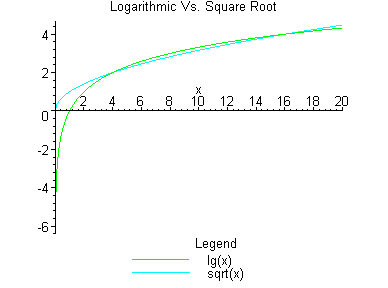
\includegraphics[scale=0.7]{log_sqrt.png}
\end{center}
\caption{The logarithmic transformation versus the square-root transformation}
\label{fig:log_sqrt}
\end{figure}

A more general transformation is the Box-Cox transformation.



Note that it is a common misconception that standard linear models assume that the data is normal. This is not the case. We will discuss in later sections that such models do not assume any distribution, but some people impose normality assumptions on the \emph{error} terms. The primary reason that it is so common to transform the data to increase normality prior to fitting a linear model is because the linear model tends to work a lot better when we have normally distributed data, although normality is not an explicit assumption of OLS.





\subsection*{What happens when we transform? Kernel density estimation example}

Suppose that we wanted to use kernel density estimation and had selected a good bandwidth. What bandwidth should we choose if we want to transform the data but retain the same amount of detail? Would it be the same? Do we just apply the same transformation to the bandwidth?

To illustrate, let's consider the model size example (whereby we were using CV to select the regularization parameter for the lasso model) which recorded how many variables were selected in the model for each parameter \textcolor{red}{or something like that...}. Suppose that we originally had a bandwidth of 3 (the left-hand plot), but we wanted to take a log-transformation of the data. The right-hand plot shows what would happen if we also log-transformed the bandwidth, so that we used a bandwidth of $\log(3)$:


\begin{figure}[H]
\begin{center}
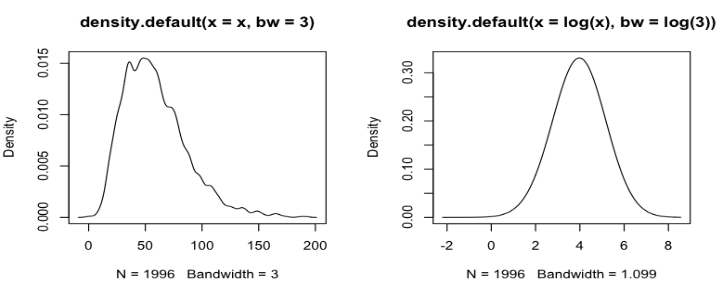
\includegraphics[scale=0.5]{log-transform-kernel.png}
\end{center}
\caption{The effect of a logarithmic transformation on the bandwidth of a kernel function}
\label{fig:log_kernel}
\end{figure}


Clearly a lot of the variance has been lost, and we have obtained a much smoother density estimate. The right-hand plot with the log-transformed bandwidth is much less variable. \textcolor{red}{Show also an example of what happens if we just don't transform the bandwidth? i.e. (x = log(x), bw = 3)}. 

How could we instead do a meaningful transformation. To answer this question, we turn to the \textbf{delta-method}. The delta method tells us how the variance of a random variable changes after a transformation, and it arises from the Taylor expansion of $g(X)$ (the details of which are shown in the appendix). In particular, suppose we have a transformation $g$ (we might have $g(x) = \log(x)$ or $g(x) = \sqrt(x)$). Suppose $X$ is a random variable such that $\mu_X = E(X)$, then the variance of the transformed random variable, $g(X)$, can be written as

$$Var(g(X)) \approx \left(g^\prime(\mu_X)\right)^2 Var(X) = Var(g^\prime(\mu_X) X)$$

For example, if $g(t) = \log (t)$, then $g^\prime(t) = \frac1t$, similarly, if $g(t) = \sqrt{t}$ then $g^\prime(t) = \frac{1}{2\sqrt{t}}$ 

This tells us that our new bandwidth should be scaled by $g^\prime(\mu_X)$. Thus, since the mean of the CV model size dataset is $\mu_X \approx 58.8$, when we take the log-transformation, we take the transformed bandwidth to be

$$h_{log} = \frac{h}{58.8}$$

and when we take the square-root transformation, we use

$$h_{square-root} = \frac{h}{2\sqrt{58.8}}$$

where $h=3$ is our original bandwidth.

Using these transformations, we obtain kernel density estimates that have the same level of variability as the original untransformed plot. In addition, the square-root transformation has also normalized the data quite nicely.

\begin{figure}[H]
\begin{center}
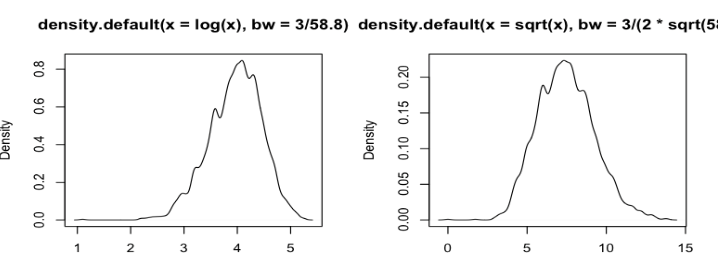
\includegraphics[scale=0.5]{log-transform-kernel2.png}
\end{center}
\caption{The effect of a logarithmic transformation on the bandwidth of a kernel function}
\label{fig:log_kernel2}
\end{figure}

Does this always work? In short: no it won't. In particular, if our estimate of the mean is extremely variable (a large standard deviation), or if the bulk of the data is far from the mean (as is the case for bimodal distributions), then the linear expansion given by the delta-method will be a poor approximation.



\section{Normalization in real life}

Often, normalization removes a lot of the natural dependence structures that exist within the data. Further, if the variables had meaningful units such that interpretations after scaling become less transparent, we might be enticed to leave the data alone.




So with this in mind, why would we ever want to normalize our data? Let's begin by giving some real-life examples.


It is probably not a reasonable assumption that the voxels are independent to one another, right? But as soon as we don't have independence, some of the most useful models are no longer applicable. Often we assume independence because we don't know how to model the dependence. Most assumptions that we make on our data are assumptions of convenience. Thus the question becomes, if the assumptions of our model are a little bit wrong, how much of an impact will this have on our conclusions drawn from these models? 


Further, what assumptions would we be making by combining the voxel responses from different sessions different people (or even from the same person)? We collected the voxel responses from a number of people, but we chose to analyze them separately. Why? The primary reason is that to combine the data from different people would mean that we had to ensure that the data were normalized (and thus comparable). But how could we do this? In a lot of applied problems, people simply collate their data from different sources together without considering whether this action makes sense.

The issue of normalization is also extremely prevalent in areas of bioinformatics, whereby each run of an experiment has different sources of bias. When the microarray technology first appeared, it was the first time scientists were able to actually look at the expression levels of multiple genes at once. The process of microarray data generation is very physical; someone must fluorescent tag the genes with chemicals and wash away the genetic materials that are not of interest. The data requires so much pre-processing and can be so noisy. \textcolor{red}{Perhaps talk about normalization in terms of microarray data more}. 

\begin{itemize}
\item {\bf Word/phrase counts from different documents}
\item {\bf Width of the stripe to normalize the gap size in fruitfly project (ongoing)}. We performed a log-transform for the gap data to make it more normal.
\end{itemize}

\begin{figure}[H]
\begin{center}
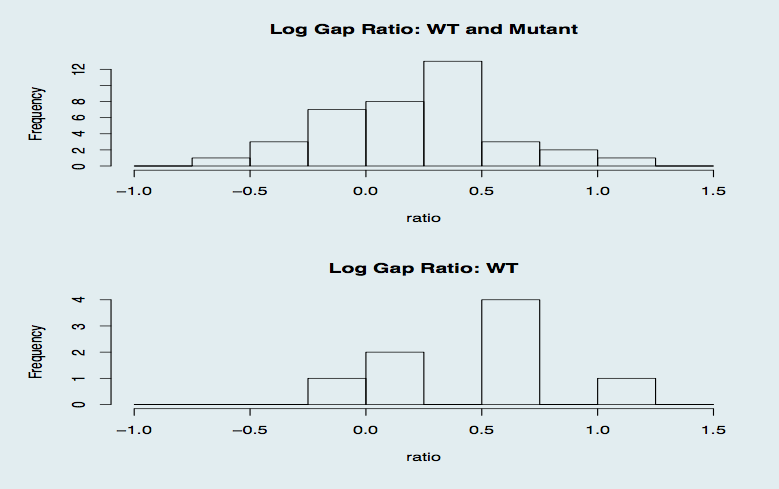
\includegraphics[scale=0.5]{gap-log.png}
\end{center}
\caption{Taking a log-transformation of the gap data}
\label{fig:log_kernel2}
\end{figure}




\section{Appendix: The delta-method}

Suppose $X$ is a random variable, where $EX = \mu_X$. A first-order Taylor expansion of $g(X)$ about $\mu_X$ is given by

$$g(X) \approx g(\mu_X) + g^\prime(\mu_X)(X - \mu_X)$$

Thus
$$E(g(X)) \approx g(\mu_X)$$

and

$$Var(g(X)) \approx g^\prime(\mu_X)Var(X)$$


To apply the delta method in reality, we don't know $\mu_X$, so we estimate it by the sample mean. In particular, this method will work well when the sample mean is close to the true mean, which will often be the case if the spread is not huge; if the variability of our estimate of the mean is small relative to the size of the mean. 

Consider, however, the example where the distribution of $X$ is bimodal. In this case, this will yield a bad approximation; since the bulk of the data will be far from this estimate of the mean.




\part{Visualization}



\chapter{Exploratory data analysis}
\label{ch:eda}



The term ``exploratory data analysis'' was brought into popular use by John W. Tukey via his book of the same name, although we would be misguided if we claimed that no-one plotted their data before Tukey came along. Visual data exploration dates back thousands of years. Humans are very visual: a large part of our brain is based on processing and interpreting what we see and we are extremely good at making judgments based on visual prompts. 

So what should we be visualizing?

\begin{itemize}
\item raw data
\item summaries of your data
\item transformations of your data
\item results of your models or algorithms
\end{itemize}

Essentially at every step of your analysis, you can do some visualization. Visualization is a great way to identify the range of your data, as well as any problems with your data: perhaps there are missing values coded as a particular integer (perhaps as ``0'' or ``999''), or strange values (perhaps someone mistyped a number). It is always a good idea to mix visualization with modeling (don't simply visualize your data and then proceed to modeling and assume that the visualization stage is over!). 

In \emph{A tour through the visualization zoo} by Jeffrey Heer, Michael Bostock and Vadim Ogievetsky (2010), the authors quote that
\begin{quote}
``Well-designed visual representations can replace cognitive calculations with simple perceptual inferences and improve comprehension, memory, and decision making. By making data more accessible and appealing, visual representations may also help engage more diverse audiences in exploration and analysis. The challenge is to create effective and engaging visualizations that are appropriate to the data.''
\end{quote}



Quotes by William Cleveland:
\begin{quote}
``Visualization is critical to data analysis. It provides a front line of attack, revealing intricate structure in data that cannot be absorbed in any other way. We discover unimagined effects, and we challenge imagined ones.''
\end{quote}

\begin{quote} 
``There are two components to visualizing the structure of statistical data – graphing and fitting. Graphs are needed, of course, because visualization implies a process in which information is encoded on visual displays. Fitting mathematical functions to data is needed too. Just graphing raw data, without fitting them and without graphing the fits and residuals, often leaves important aspects of data undiscovered.''
\end{quote}

\textcolor{red}{Expand on these and make more connections!}

In summary:
{\bf Visualization should be your first choice for your analysis when writing papers, giving presentations \emph{and for life}.}


\section{A good graph is worth a thousand words: examples of visual data}

\subsection*{Giuseppe Piazzi, Gauss and the discovery of Ceres}

In 1801, Giuseppe Piazzi, an Italian Catholic priest, mathematician and astronomer, observed three sightings of a new ``planet'', and he recorded its positions in the sky and the time at which he saw it. The image below from Tennenbaum and Director, 1997, shows the three positions of Ceres observed by Piazzi. This is an example of visualization of data. It's not just boxplots and histograms (although they are informative too), we also want to simply \emph{look} at what we are analyzing. What he observed was that this particular planet was moving slowly counter-clockwise against the ``sphere of the fixed stars''. This would have been very difficult to convey in text or numerical form, this visual representation is the most informative way of representing this data. We are given context such as the location of other stars relative to the new planet. 


\begin{figure}[H]
\begin{center}
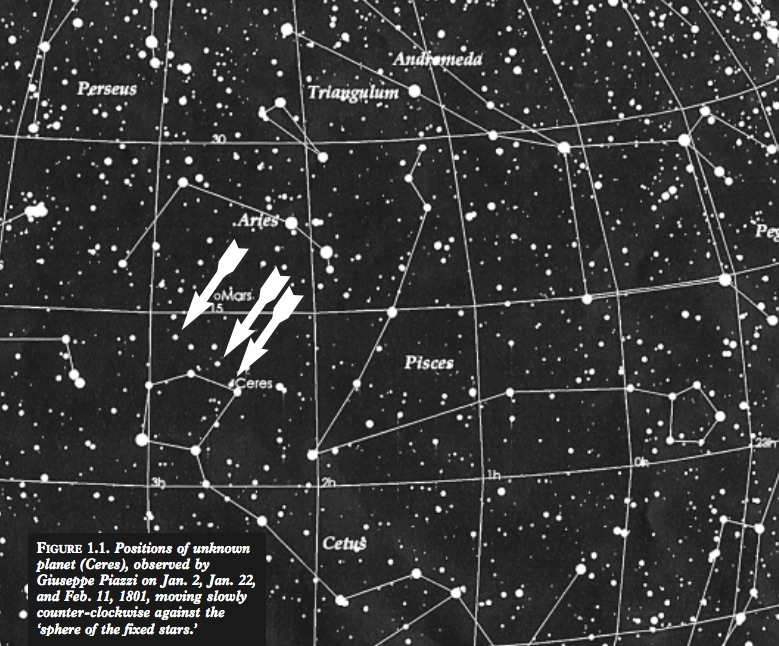
\includegraphics[scale=0.4]{ceres.jpg}
\end{center}
\caption{Ceres}
\label{fig:ceres}
\end{figure}

Piazzi was in fact making a lot of assumptions based on his observations. He assumed that the planets observed at the three different locations were the same, but why? There are a lot of alternative theories he could have come up with.

In fact it was Carl Friedrich Gauss, a German mathematician and physical scientist who made significant contributions to many fields (including number theory, algebra, statistics, analysis, differential geometry, geophysics, electrostatistics, astronomy and optics) who actually showed, using Piazzi's three data points, that the three planets observed by Piazzi were one in the same; Ceres. He used Kepler's second law of planetary motion to describe the trajectory of Ceres.

In fact, Gauss was using \emph{Least Squares} to describe Ceres' trajectory. Isn't it amazing that these Gauss and Piazzi were able to get so much information from only \emph{three data points}. They certainly didn't need ``big data''! It's not really about how much data you have, but rather it's about how much information each observation contains.


\subsection*{Napoleon's invasion of Russia}

You could write entire books to even summarize the events in Napoleon's invasion of Russia, but to obtain a concise, yet complete, summary, visualization offers far superior tools as Charles Minard's map (below) shows. Here, Minard is able to simultaneously plot in two dimensions six different types of data. The plot contains substantial amounts of information about the progression of Napoleon's army. There is geographic information (the distance traveled, the longitude and latitude), the direction of travel, the number of troops in Napoleon's army, the temperature and the location relative to specific dates.



\begin{figure}[H]
\begin{center}
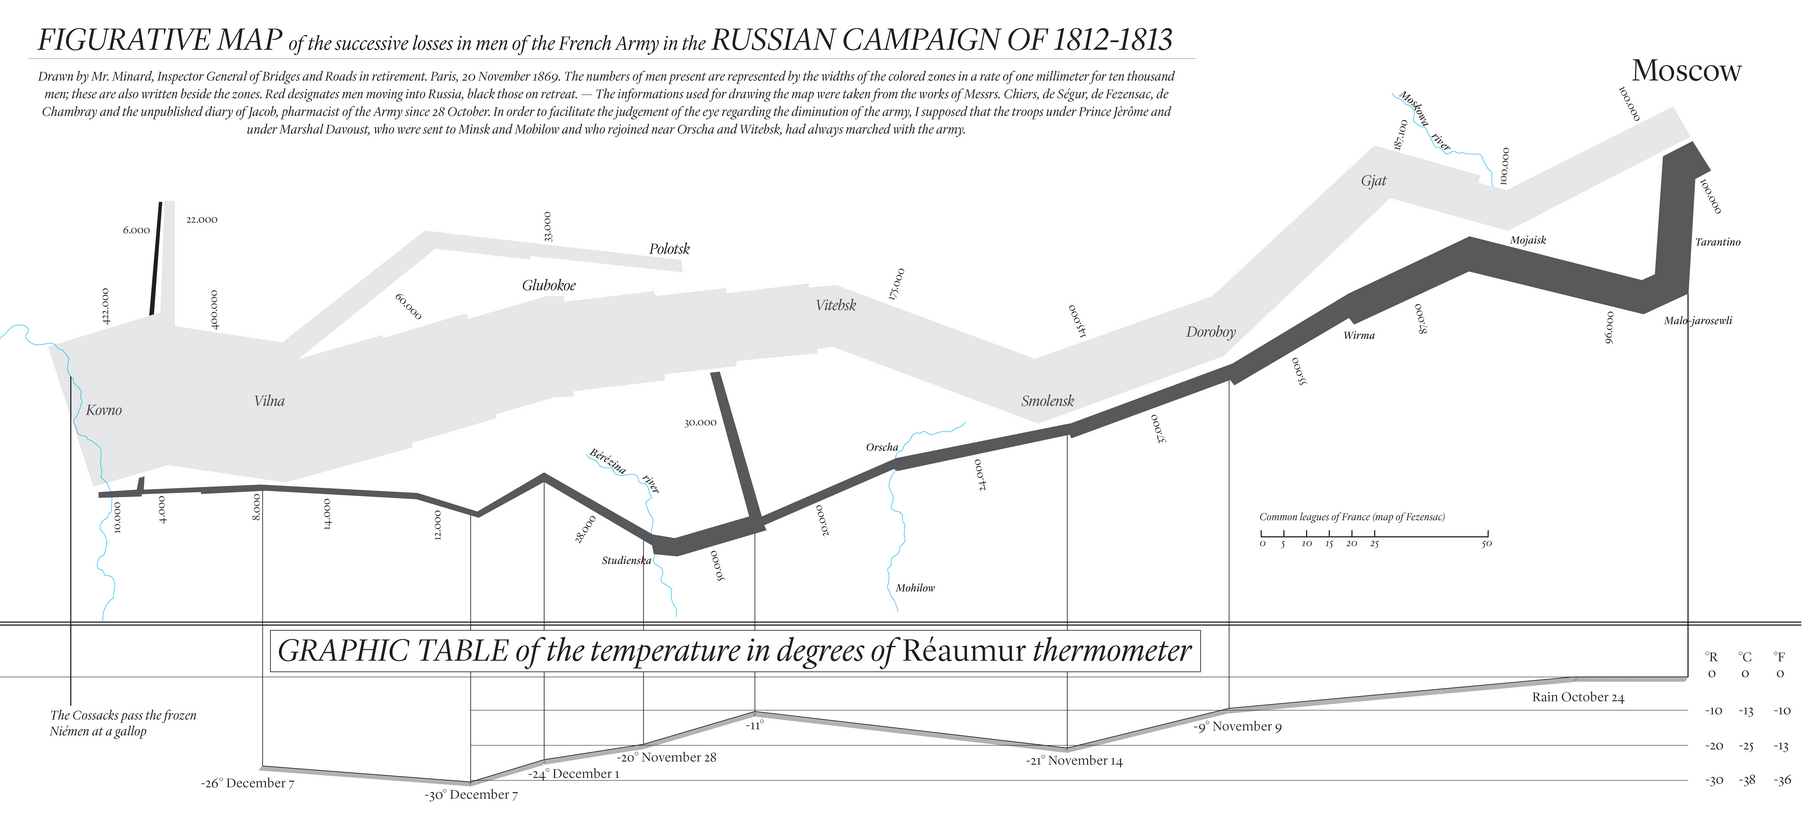
\includegraphics[scale=0.2]{napoleongood.png}
\end{center}
\caption{The progression of Napoleon's army}
\label{fig:napoleon}
\end{figure}

However, not all graphics are created equal. Below we show another example of a plot designed to show the same information. Although Minard's plot above removes some of the detailed geographical information, it actually portrays the the viewer the information in a more concise but substantially more interpretable and understandable way. The map below is too noisy and cluttered that it becomes confusing and it is difficult to extract the useful information.


\begin{figure}[H]
\begin{center}
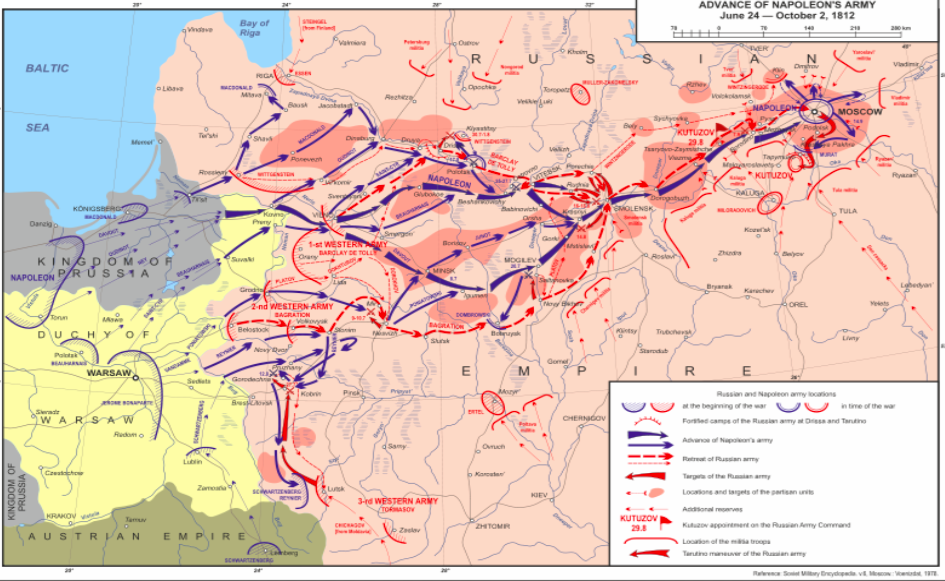
\includegraphics[scale=0.3]{napoleon.png}
\end{center}
\caption{The progression of Napoleon's army (confusing version)}
\label{fig:napoleon}
\end{figure}



\section{Tools for visualizing data}

There are a wide array of tools available in multiple programming languages for visualizing data. The examples we present are based on the R programming language. 

There are a number of considerations that one should take into any plotting adventure. Here we list a few: \textcolor{red}{Fix up!}

\begin{itemize}
\item Continuous values are better mapped into continuous gradient scales, whereas discrete colors should be used to represent different categories.
\item Bright colors draw attention better than dull colors. For example, if you wish to have the viewers attention drawn to a particular point, color it in a bright color!
\item Transparency and point size (for example in scatterplots) should be utilized for large datasets so that more information can be portrayed without overplotting becoming an issue.
\item A smoothing line provides information about the overall trend present in scatterplots or time series plots, especially when there are many data points overplotted on top of one another.
\item Brushing can be used to effectively bring in other variables.
\item Motion (such as movies) an bring out structures that static representations cannot.
\end{itemize}

If you're using R, you should really be using the data visualization package ggplot2 designed by Hadley Wickham rather than the base R plotting tools. Many of the above considerations can be irritatingly difficult to achieve in most plotting languages but are incredibly easy and natural (not to mention aesthetically pleasing!) with ggplot2. 

Often the most effective visualization tools are the simple ones.

\subsection*{Scatterplots and smoothing}

Scatterplots are likely to be one of the first types of exploratory data analysis that you were exposed to. Traditional scatterplots involve plotting one variable against another, however as data is becoming more and more complex, many extensions to this traditional, yet useful, plot have begun to take hold. For example, making use of transparency and color is an extremely useful way to demonstrate concentrations of points as well as categorical information and may even add another continuous variable into the plot.

For example, the plot below shows a number of scatterplots without transparency. There are so many points plotted on top of one another that it becomes difficult to visually determine the trend.

\begin{figure}[H]
\begin{center}
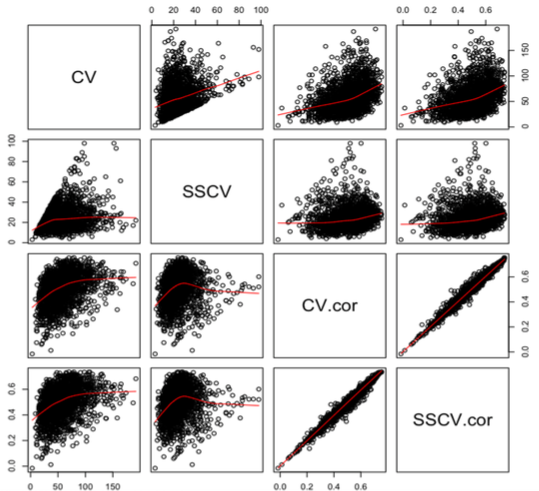
\includegraphics[scale=0.5]{pairs.png}
\end{center}
\caption{Scatterplot without transparency}
\label{fig:pairs}
\end{figure}

When we add transparency, it becomes much easier to identify patterns in the data as well as regions where the data are more condensed.

\begin{figure}[H]
\begin{center}
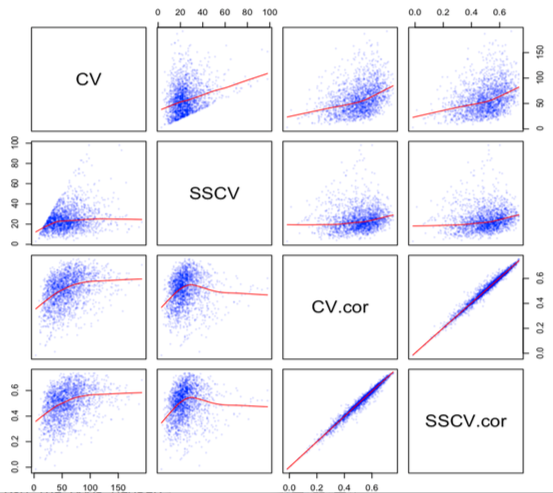
\includegraphics[scale=0.5]{pairs2.png}
\end{center}
\caption{Scatterplot with transparency}
\label{fig:pairs2}
\end{figure}


Further, the above plots each contain a red smoothing line, which can be extremely useful to emphasize the trend of the data. We will come back to the notion of smoothing later.




\subsection*{Histograms}

\begin{itemize}
\item Shows you how much data you have
\end{itemize} 

\subsection*{Kernel estimation}


What if, instead of looking at histograms, we estimated the density and plotted that instead:


\begin{figure}[H]
\begin{center}
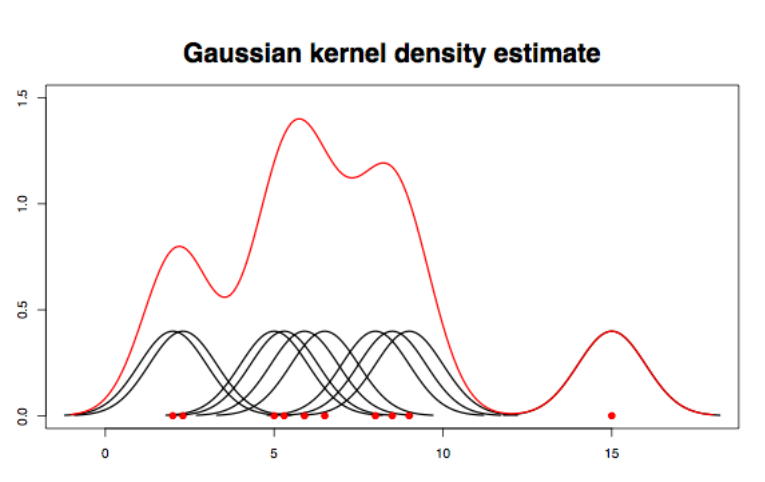
\includegraphics[scale=0.5]{voxelkernel.png}
\end{center}
\caption{Kernel density estimation}
\label{fig:kernel}
\end{figure}


The above example corresponds to Gaussian kernel density estimation for 10 data points (the red points plotted along the x-axis). For each data point, a Gaussian curve is plotted centered at the data point (these are the black curves). The spread of the curves is defined by the \emph{bandwidth} (see blow). The Gaussian kernel density estimate (the red curve) is then obtained by adding the height of the black curves.





Although in the example above, we have used Gaussian curves, there is no need to make this restriction. To define the general kernel density estimator, we first define a 1-dimensional kernel function, $K(\cdot)$, which satisfies
$$\int K(t) dt = 1 ~~~~~~~ \int t K(t) dt = 0$$

That is, we can think of the kernel function as a density that integrates to 1 and that corresponds to distribution has expected value 0. For the Gaussian example above, this would be the Gaussian density function.

We next define the re-scaled kernel function with bandwidth $h$ (the bandwidth describes the spread of each individual curve) to be
$$K\_h(t) = \frac{1}{h} K\left( \frac{t}{h} \right)$$

so that a kernel density function of data (where we can notationally define the data by $x\_1, x\_2, ..., x\_n$) is defined to be 
$$g\_{n, h}(x) = \frac{1}{n} \sum\_{i=1}^n K\_h(x\_i - x)$$


From the formula above, we can see that the height of the kernel density estimator curve at a given $x$ is influenced by the height of each individual kernel curve at our data point $x\_i$ for $i = 1, ..., n$ (note that $x$ is our parameter, which we vary to trace out the kernel density curve, while the $x_i$ are the individual data points). In particular, assuming that the individual kernel functions, $K_h$, are centered at $x_i$, then the closer our location, $x$, is to a given point $x_i$, the more height the kernel function for $x_i$ will contribute.

The tuning parameter is the bandwidth, $h$. A small $h$ corresponds to very condensed spread (as if you're squeezing the kernel function), and a large $h$ corresponds to an elongated spread. 



\begin{figure}[H]
\begin{center}
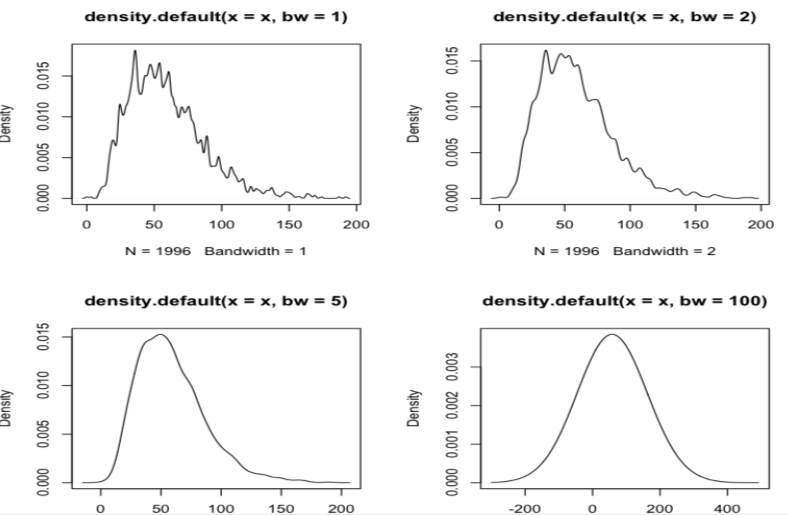
\includegraphics[scale=0.5]{bandwidth.png}
\end{center}
\caption{Comparison of different bandwidths}
\label{fig:bandwidth}
\end{figure}

It is easy to implement kernel smoothing estimators in R, and the only hard part stems from choosing the value bandwidth, $h$. There is currently no overall method for automatically selecting the bandwidth, and in general it is recommended that you try several and use your judgment to choose which one is the best fit for the data. For example, in the image above, the bandwidth of 1 is far too small, it is capturing all of the noise in the data. 

Note that we often call the bandwidth, $h$, a regularization parameter (we will see this again when discussing lasso and ridge linear models). Regularization parameters typically represent a tradeoff between bias and variance in our estimation. For example, from the image above, we see that the kernel density estimators with small bandwidth have very high variance (the curve jumps around a lot), but low bias (on average, the value of the kernel is close to the true value of the density). On the other hand, the kernel density estimators with large bandwidth have very low bias (the curve is very smooth and much less noisy) but have high bias (on average, the value of the kernel estimator might be quite far from the true value of the density). 




By using kernel density estimation we are in essence assuming that our data are realizations of a sequence of random variables, $X_1, X_2, ..., X_n$. It is important to question whether this even makes sense for the data at hand. If the answer is yes, begin to pry information such as what is the sampling model? Where does the randomness come from?

Let's change the notation for our kernel density estimation by assuming that our observations are in fact realizations of random variables, $X_1, X_2, ..., X_n$, with a density function, $f$. Then kernel density estimation is trying to estimate $f$ using

$$\hat{f}_{n, h}(X) = \frac{1}{n} \sum_{i=1}^n K_{h}(X_i - x)$$


Is $\hat{f}_{n,h}(x)$ a random variable? Yes is is, because it is a function of the random variables $X_i$. Is $\hat{f}_{n, h}(x)$ a good estimator for $f$? Firstly, the answer to that question depends on what we mean by "good": do we mean an estimator with low bias, an estimator with low variance, or perhaps a combination of the two?



\subsubsection*{Regularization}



We mentioned above that short bandwidths correspond to an estimator, $\hat{f}_{n, h}(x)$, of $f$ that has low bias, but high variance, whereas long bandwidths corresponds to an estimator that has high bias but low variance. Is one of these two extremes better than the other? Is it possible to obtain a happy mid-ground between the two? This is where the bias/variance trade-off comes in: perhaps we would rather find an estimator that minimizes a combination of the bias and the variance, such as the mean squared error (MSE):

$$\text{MSE} = \text{Bias}^2 + \text{Variance}$$

In fact, in modern statistics, gains are often obtained by increasing bias, but reducing variance. We can add a regularization (or smoothing) parameter to control the trade-off between bias and variance (we will return to this concept when we discuss the lasso linear model).





\subsubsection*{The bias-variance tradeoff for kernel density estimation}



In particular, the mean squared error for the kernel estimator can be approximated by


\begin{align*}
\text{MSE} &= \text{Bias}^2 + \text{Variance} \\
& \approx \left[ \frac{1}{4} \sigma^4_K \left(f^{\prime \prime}(x)\right)^2\right] h^4 + \frac{1}{nh} \left[ \int K(u)^2 f(x) du \right]
\end{align*}


which shows that the bias increases with the bandwidth, $h$, while the variance decreases with $h$. 

The mathematical steps are presented in the appendix at the end of this section for curious readers, but could easily be skipped without much loss of conceptual understanding.


Next, the pointwise MSE risk function above can be shown to be optimized asymptotically by a bandwidth (depending on $x$) given by

$$h^*(x) = \left( \frac{c_2(x)}{c_1^2c_3(x) n} \right)^{\frac15}$$

where

$$c_1 = \int t^2 K(t) dt = \sigma^2_K, ~~~~~~ c_2(x) = \int K^2(t) dt f(x), ~~~~~~ c_3(x) = \left(f^{\prime \prime}(x) \right)^2$$

Kernel density estimation is well-known to perform poorly at the boundaries of your dataset where there is little data available. The algorithm tends to extrapolate out from the denser regions.

\subsubsection*{The optimal kernel function}




Further, does there exist an optimal kernel function. In our introductory example, we used a normal density with variance 1, but how do we know that a normal density with variance 2 wouldn't be better? In the end, this wouldn't make any difference, it would just correspond to a scale change. In fact, Maron and Nolan's (1989) work showed that the optimal kernel was that which minimizes

$$T(K) = \left\{ \| K \|_2^8 \sigma^2_K \right\}^{\frac15}$$

and that this optimal kernel is given by the Epanechnikov kernel:

$$K(t) = \frac34 \frac{1}{5^{1/5}} \left( 1 - \left(\frac{t}{15^{1/5}}\right)^2\right) I_{\left(\vert t \vert \leq 15^{1/5}\right)}$$

However, the asymptotic efficiency lost for other kernels is minimal. In fact R uses the cosine kernel below, which has an efficiency ratio of 1.0004 relative tot he optimal:

$$K(t) = \frac12 \cos(t) I_{\left(\vert t \vert \leq \frac{\pi}{2}\right)}$$

In the figure below, the black curve is the Epanechnikov kernel function and the red curve is the cosine kernel function.


<img src="kernel.png" alt="Kernel" style="width:300px;height:200px;">


\begin{figure}[H]
\begin{center}
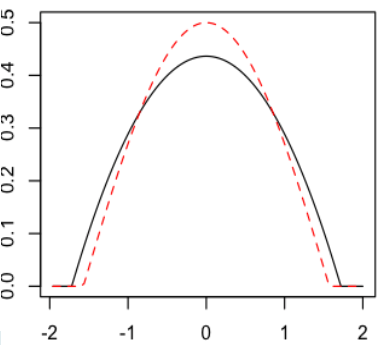
\includegraphics[scale=0.5]{kernel.png}
\end{center}
\caption{Kernel}
\label{fig:kernel}
\end{figure}

The optimal (minimax) MSE rate for smooth density functions with $s$-derivatives is $O\left( n^{-\frac{2s}{2s + d}}\right)$, where $d$ is the dimension and $s$ is the smoothness. When $s$ gets large (so that the density function is really smooth), we get a rate close to $\frac{1}{n}$, which is the familiar parametric (assuming normality) rate. When $d$ is large (the data is high-dimensional), then $\frac{2s}{2s + d} \rightarrow 0$, implying a very slow rate. In essence: if your data does not have a low-dimensional structure, then estimating its density function is hopeless!

For example, if your data has 26,000 dimensions (not uncommon in bioinformatics data), and $s = 1$ with $n = 2,000,000$, then our rate is $2,000,000^{-\frac{2}{26,000}} = 0.9988846$, which is very far from 0!



In fact, it is an active research area to attempt to find informative low-dimensional structures that are embedded in high dimensions. In many cases where we have ``big data'', the datasets themselves are huge, but we are really interested in the hidden, low-dimensional structures contained within.


\subsubsection*{Questions}

\begin{itemize}
\item  How could you use cross-validation to select the bandwidth, $h$?
\end{itemize}






\subsection*{Scatterplots and smoothing}

We mentioned that it is often a good idea to add a smoothing line to scatterplots. But how do we come up with the smoothing line? There are actually a number of methods, but we can use kernel density estimation.

For example, given pairs of data points $(x_i, y_i)$, $i = 1, ..., n$, where $x_i$ might be a father's height and $y_i$ might be his son's height. Suppose that we are interested in predicting the son's height based on the father's height. Then we might fit a model which predicts $y$ based on $x$ using the Nadaraya-Watson kernel smoother with bandwidth $h$:

$$\hat{y}(x) = g_h(x) = \frac{\sum_{i=1}^n K_h(x_i - x) y_i}{\sum_{i=1}^n K_h(x_i - x)}$$

This equation corresponds to a predicting $\hat{y}$ given some value $x$ to be the weighted average of the $y_i$'s where $y_i$'s which have correxponding $x_i$'s that are close to our $x$ of interest have larger weights and thus contribute more (since $K_h$ is centered about $0$). 

For any fixed $x$ value, the above prediction for $\hat{y}$ corresponds to finding the (local) constant minimizer of a weighted least-squares over $\theta$:

$$\hat{y} = \underset{\theta}{\text{argmin}} \sum_{i=1}^n (y_i - \theta)^2 w_i(x) ~~~~~~ \text{where} ~~~~~ w_i(x) = K_h(x_i - x)$$


That is, for each fixed $x$, we want to find the value, $\hat{y}$, which is the closest (in terms of the squared distance) to the $y_i$'s whose corresponding $x_i$'s are close to our $x$ of interest. We can call this function a ``smoothing'' function, since it is taking into account all possible values that we have observed and averaging them based on how close their $x_i$'s are.
\textcolor{red}{Make Figures!}


Instead of finding a constant fit, we could instead do a local polynomial fit, for example, finding


$$\hat{y} = \underset{\theta}{\text{argmin}} \sum_{i=1}^n \left(y_i - \sum_{j=1}^p \beta_j(x_i - x)^j\right)^2 w_i(x) ~~~~~~ \text{where} ~~~~~~ w_i(x) = K_h(x_i - x)$$

where $p=0$ gives the NW kernel smoother, $p=1$ gives the local linear smoother. The idea is that you want to fit a local polynomial to a subset of the data near the point whose response is being estimated. The polynomial is fitted using least squares, giving more weight to the points near the point whose response is being estimated, and less weight to points further away. \textcolor{red}{Give examples of polynomial smoothing for different weights and different degrees}. 


Similar to our discussion of kernel density estimation above, we can use Taylor expansion to obtain the bias and variances of these kernel smoothers:


Suppose that we are estimating a function $f$ using a non-parametric regression model

$$Y_i = m(X_i) + \epsilon_i$$

where $m$ is a ``smooth'' mean function and $\epsilon$ is the error term with mean zero. Assume that $X_i$ and $Y_i$ are IID and $X_i$ jas a density $f$ and $Var(Y | X = x) = \sigma^2$, then under necessary regularity conditions we have the following (pointwise) bias-variance tradeoff:

For the Nadaraya-Watson kernel the bias is given by
$$\text{Bias}_{\text{NW}} = \left(m^{\prime \prime} + \frac{2 m^\prime(x) f^\prime(x)}{f(x)} \right) b_n$$ 

which means that for the local-linear estimator (where $f(x)$ is constant), we have

$$ \text{Bias}_{\text{linear}} = \left(m^{\prime \prime}\right) b_n$$

where $b_n = \frac12 \sigma_K^2 h^2$ and the variance for both methods is 
$$V_n = \frac{\sigma^2(x)}{f(x) n h } \int K^2(t) dt$$


Thus we have this term $b_n$ which is directly related to the bandwidth $h$, which implies that the bias for both methods is increases to $h$.

Can you see the similarity between smoothing and kernel density estimation? What are the differences?

\textcolor{red}{This needs a lot of work and/or simplification}


\subsection*{Boxplots}

The boxplot is a simplified histogram that is particularly good for comparing two samples. The boxplot contains a lot of information about the range and spread of the data. In the middle of the ``box'', we have a line corresponding to the median, and the edges of the box correspond to the upper (third) and lower (first) quartiles, $q_{0.75}$ and $q_{0.25}$, respectively. The inter-quartile range (IQR) is the difference between the third quartile and the first quartile. The box contains ``whiskers'', which extend $1.5 \times IQR$ from the edges of the box. Any ``outlier'' values larger than $q_{0.75} + 1.5 \times IQR$ or smaller than $q_{0.25} - 1.5 \times IQR$ are drawn as dots. The figure below uses side-by-side boxplots to show a comparison of two sets of observations. Here we are comparing the number of observations selected by two feature selection methods (one based on cross-validation (CV) and the other based on a stability-based cross-validation (SSCV) approach).


\begin{figure}[H]
\begin{center}
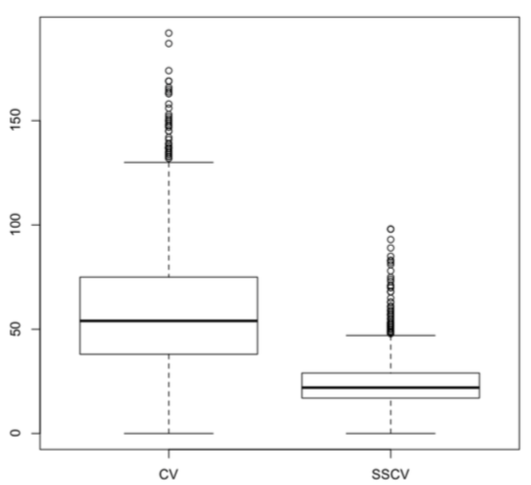
\includegraphics[scale=0.5]{boxplot.png}
\end{center}
\caption{Boxplots}
\label{fig:boxplot}
\end{figure}

It is clear that the SSCV method selects significantly fewer observations than the CV method. the CV method also exhibits more variability than the SSCV method.

As a warning, such comparisons can be misleading if the two samples that we are comparing are not similarly normalized or are not directly comparable. Recall our discussion on normalization and comparability in the data wisdom excerpt. For example, suppose we have done a microarray gene expression experiment, where we have obtained the data in batches. Before comparing different samples, it might be a good idea to do some pre-processing to make the samples comparable, otherwise the differences that you are observing between the two samples may be a ``batch effect'' rather than actual differences in gene expression.

\subsection*{Q-Q plots}

Q-Q plots are kind of fancy! They really take advantage of our visual desire to seek straight lines. We are much better at detecting straight lines than we are at detecting, say, polynomials.

Suppose that we have a dataset and we want to check whether or not it follows a particular distribution. The general idea is to compare the quantiles in your data from the quantiles of the distribution. If these match (i.e. the plot of one versus the other follows a straight diagonal line), then you can be reasonably certain that your data follows the distribution of interest.

For example, the gap data from the fruitfly project before (top) and after (bottom) taking a log-transform.

<img src="gap-qq.png" alt="QQ plot log-transformed gap data" style="width:600px;height:800px;">

\begin{figure}[H]
\begin{center}
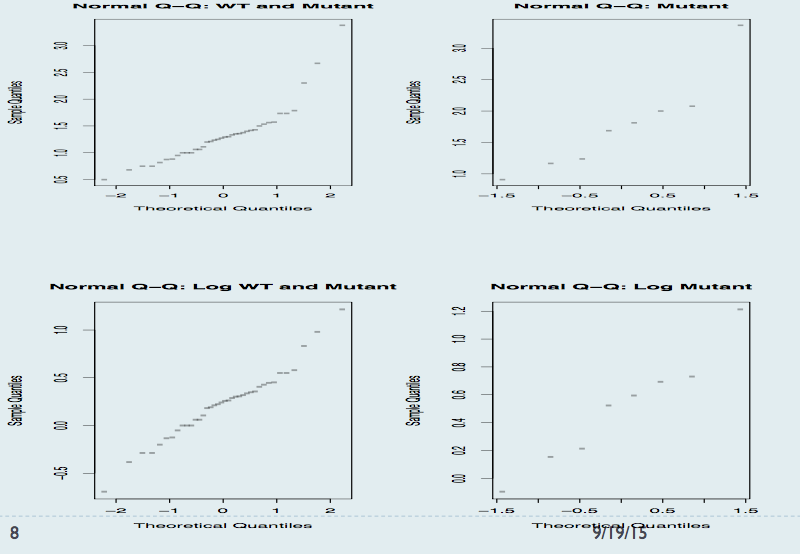
\includegraphics[scale=0.5]{gap-qq.png}
\end{center}
\caption{Q-Q plots for the gap data}
\label{fig:qq}
\end{figure}

We can see that the two bottom plots correspond much more to a straight line than do the top two (pre-transformed plots). This tells us that the transformed variables more accurately follow a normal distribution (the diagonal line is a lot more straight) than do the pre-transformed variables.





\section{ggplot2 in R}






\section{Appendix: the bias-variance tradeoff for kernel estimation}


\subsection*{The bias of $\hat{f}$:}

The expected value of $\hat{f}_{n, h}(x) = \frac{1}{n} \sum_{i=1}^n K_h(X_i - x)$ is given by


\begin{align*}
E(\hat{f}(x)) &= E\left( \frac{1}{n} \sum_{i=1}^n K_h(X_i - x) \right)\\ 
              &= \frac{1}{n} \sum_{i=1}^n E(K_h(X_i - x)) \\
              &= E(K_h(X_1 - x))
\end{align*}

where we have used both the linearity of expectation in the second equality and the fact that the $X_i$ are IID in the third equality.

Continuing, we get that


\begin{align*}
E(\hat{f}(x))  & = E(K_h(X_1 - x))  \\
                     & = E\left( \frac{1}{h} K\left(\frac{X_1 - x}{h}\right) \right) \\
                     & = \int \frac{1}{h} K\left( \frac{z - x}{h} \right) f(z) dz \\
\end{align*}


Using the change of variables $u = (z - x)/h$, we get that



\begin{align*}
E(\hat{f}(x)) & = \int K\left( u \right) f(x + hu) du \\ 
\end{align*}

which implies that the expected value of $\hat{f}$ is an average of $f$ locally around $x$, however this integral is not analytically solvable so we use a Taylor expansion of $f(x + hu)$ in the argument $hu$, which is valid as $h \rightarrow 0$:

$$f(x + hu) = f(x) + f^{\prime}(x) hu + \frac12 f^{\prime\prime}(x) h^2 u^2 + \text{smaller order terms} $$

Thus substituting this into our equation for $E(\hat{f}(x))$, we end up with


\begin{align*}
E(\hat{f}(x)) & \approx \int K\left( u \right) \left[ f(x) + f^\prime(x) h u + \frac12 f^{\prime \prime}(x) h^2 u^2 \right] du \\ 
& \approx f(x) + \frac{f^{\prime \prime}(x)}{2} h^2 \int K(u) u^2 du 
\end{align*}


since $\int K(u) du = 1$ and $\int u K(u) du = 0$, by definition. Thus the bias of $\hat{f}$ is given by

$$\text{Bias} = E(\hat{f}(x)) - f(x) = \frac{f^{\prime \prime}(x)}{2} h^2 \int K(u) u^2 du  + \text{smaller order terms}$$

Surprisingly, the bias does not depend on $n$, the number of samples. So no matter how large our sample is, the expected value of our density estimator will not get closer to the true density value.

\subsection*{The variance of $\hat{f}$}


Similar calculations show that the variance of $\hat{f}$ is


\begin{align*}
\text{Var}(\hat{f}(x)) &= \text{Var}\left( \frac{1}{n} \sum_{i=1}^n \frac{1}{h} K \left( \frac{X_i - x}{h} \right) \right)\\
& = \frac{1}{n^2h^2} \sum_{i=1}^n \text{Var}\left( K \left( \frac{X_i - x}{h} \right) \right)
\end{align*}


where we can take the sum out of the variance expression because the $X_i$ are IID. Continuing, we have


\begin{align*}
\text{Var}(\hat{f}(x)) &=  \frac{1}{n}  \text{Var}\left( \frac{1}{h} K \left( \frac{X_1 - x}{h} \right) \right) \\
& = \frac{1}{n}  E \left( \frac {1}{h}K \left( \frac{X_1 - x}{h} \right) \right)^2  \\
&= \frac{1}{h} \int K\left( \frac{z - x}{h} \right)^2 f(z) dz\\
& = \int K(u)^2 f(x + hu) du\\
& = \int K(u)^2 \left[ f(x) + f^\prime(x) h u + \frac12 f^{\prime \prime}(x) h^2 u^2 \right] du\\
& \approx \int K(u)^2 f(x) du 
\end{align*}

Thus the variance can be approximated by



\begin{align*}
\text{Var}(\hat{f}(x)) &\approx \frac{1}{nh} \left[ \int K(u)^2 f(x) du \right] 
\end{align*}



The variance depends on $\frac{1}{n}$ as well as $\frac{1}{h}$. So that the more samples we have, the smaller the variability of our estimator, and the larger the bandwidth, the smaller the variability of our estimator. You might say that $nh$ has become our effective sample size: this has nothing to do with getting the value that we want (recall that bias does not depend on $n$), but it has a lot to do with reducing the variance.




\subsection*{Mean squared error calculation}

The question becomes, how to you choose $h$ so that the bias and variance are both small? Recall that a small $h$ will correspond to low bias but high variability, whereas a large $h$ corresponds to a high bias but low variability. The solution in general is to try to minimize a combination of the bias and variance, called the mean squared error (MSE), defined to be
$$MSE(\hat{f}) = E\left(\hat{f} - f\right)^2$$

(note that this looks a lot like the variance, $E\left(\hat{f} - E(\hat{f})\right)^2$, and in fact, the MSE is the variance when $\hat{f}$ is unbiased, i.e. $E(\hat{f}) = f$).

Finally, putting the above calculations together, we obtain an expression for the mean squared error:


\begin{align*}
\text{MSE} &= \text{Bias}^2 + \text{Variance} \\
& \approx \left[ \frac{1}{4} \sigma^4_K \left(f^{\prime \prime}(x)\right)^2\right] h^4 + \frac{1}{nh} \left[ \int K(u)^2 f(x) du \right] 
\end{align*}


where $\sigma^2_K = \int u^2K(u) du$.

Here we see that the bias term is large when $h$ is large and the variance term is small when $h$ is large.


\section{Notes}

A number of excellent resources for data visualization exist. Some of the traditional, yet still relevant, texts include \emph{The future of data analysis} by Tukey (1962), \emph{Envisioning information} by Edward R. Tufte (1990) and \emph{Visualizing data} by William S. Cleveland (1993). Some more modern references include \emph{A tour through the visualization zoo} by Jeffrey Heer, Michael Bostock and Vadim Ogievetsky (2010). For those interested in learning more about graphics in R, you need look no further than the works by Hadley Wickham, including his book \emph{ggplot2: Elegant Graphics for Data Analysis (Use R!)} (2009) and that of his collaborators including the \emph{R Graphics Cookbook} by Winston Chang (2013).

For references on kernel density estimation, see M. Rosenblatt (1956)'s \emph{Remarks on some nonparametric estimates of a density function} , and E. Parzen (1962)'s \emph{On estiamtion of a probabilty density function and mode}.





\section{Answers to the questions:}

\begin{itemize}
\item  \textbf{What are the similarities and differences between kernel density estimation, kernel regression estimation and local regression?}\\
First, in all situations the problem is both to estimate $y$ given $x$. Further, kernel regression is a special case of local regression. All three aim to exploit the tradeoff between bias and variance though a smoothing or regulatization parameter. The first two approaches manipulate the bandwidth of a kernel function whereas the smoothing spline for local regression also trades of bias and variance using a smoothing parameter (which controls the global smoothness of the function). What about some differences? The main difference is that the kernel density estimator generates its estimates using only the information from $x$, while kernel regression utilises both $x$ and $y$.
\item \textbf{How could you use cross-validation to select the best bandwidth?}\\
First, we need to define a measure of how good a particular density estimator is performing. Recall our discussion on using the KL-divergence to measure the distance from the true distribution to the estimated distribution. We concluded that the best distribution will correspond to that with the parameter, $\theta$, which minimizes the negative log-likelihood. Thus we can use the negative log-likelihood as a measure of prediction performance. In particular, the density with bandwidth, $h$, that yields the largest negative log-likelihood corresponds to the density that is closest (in KL-distance) to the true density.\\
How does cross-validation come into this? Suppose we have split our dataset into 10 subsets. We can temporarily remove the first subset, and calculate the density estimator function for various values of $h$. We can then use the withheld subset to calculate the negative log-likelihood for each $h$, (that is, calculate -$\hat{f}_h(x_{\text{witheld}})$) and identify which $h$ yields the largest value. This will be the $h$ that we select for that particular fold. We could then repeat this, withholding instead the second subset of the data, and come up with a new optimal $h$. Eventually, we will have 10 different optimal bandwidth values (hopefully they're not too different from one another), and we could average them to obtain our final bandwidth, $h$.
\end{itemize}






\part{Finding structure in data}



\chapter{Principal component analysis}
\label{ch:pca}



Principal component analysis (PCA) is one of the most widely used methods for dimensionality reduction. Why might we want to reduce the dimension of our data? Doesn't that mean that we're losing information? Well... yes, but this can be a good thing if what we're throwing away is the bits of our data that aren't useful! When we have more concise information, it is more interpretable, and if we can effectively condense our masses of information into smaller, more concise, parcels of information then that's just great! Dimensionality reduction is used for a huge array of reasons including visualization, faster computation, smaller storage and faster communication of data and it can even be considered to be a form of regulatization (by indirectly reducing the variance of our estimation).

The idea behind PCA is that we want to decompose our variables into informative orthogonal components consisting of linear combinations of the original variables. We want to find the components which posess the smallest ($L^2$) distance from the original data. There are a number of different algorithms to produce these components for example by using singular value decomposition (SVD) or eigen decomposition: Let $G = X^TX$ be the sample covariance matrix which is symmetric. The eigenvalue decomposition of $G$ is given by

$$G = UDU^T$$

where $U$ is unitary or orthogonal matrix (that means $U^TU = I$) and $D$ is a diagonal matrix with non-negative diagonal entries that are the eigenvalues of $G$. Let the $j$th column vector of $U$ be $U_j$ and of $D$ be $d_j$, that is

$$GU_j = d_j U_j$$

The principal components are linear combinations of the original variables in our data, and the idea is typically that we want to use some of these principal components as our new variables (typically those that capture the most variability within the data). Why might we be weary of considering linear combinations of our data, rather than considering each variable individually? One of the primary reason is that we lose interpretability. What does a principal component measure? 

The first principal component is the linear combination of the variables that captures the most variability within the data, while the second principal component is the linear combination that captures the most variability that is not captured (or is left over) by the first principal component, and so on and so forth. 

Another way to think about the principal components is that we want to find the projection of the data such that along that projection, the variability is maximized. 

It is common to center the data prior to conducting PCA. 

Let's walk through the theoretical steps: \textcolor{red}{Do it}

\begin{itemize}
\item talk about looking at how much variability each PC captures (screeplot -- plot the eigenvalues in decreasing order -- inspect to find a gap to decide how many principal components to keep)
\end{itemize}



PCA has a huge array of uses in the realm of dimensionality reduction. It is widely used and is ideal for multivariate Gaussian data with degeneracy. It is incredibly useful for visualization of complex datasets. 



\section{PCA for the Enron Data}

In 2001, the US energy company \emph{the Enron Corporation} was caught up in a corruption scandal that led to the bancruptcy of the company. The company used accounting loopholes, special purpose entities and poor financial reporting to hide billions of dollars in debt from failed deals and projects. As a result of the investigation, a large portion of the corporation's emails between November 1998 and June 2002 became public. 

The emails create a directed network on 154 employees, so our data consists of a $154 \times 154$ matrix, $E$, consisting of Enron employees and their positions within the corporation. Let's define the adjacency matrix $A$ where $A_{ij}$ is the number of emails from person $i$ to person $j$. Below we will use PCA on the matrix $A$ to explore the data and learn about the employees.

If we conduct PCA on $A$, the sum of the variance captured by the first two principal components is 71.6\% of the total variability in the data (the top left screeplot belop shows that the first two components capture a substantial amount of the information). Employee 20 dominates the first principal component (the outlier in the upper right corner of the plot of PC1 against PC2), and the second principal component is dominated by Employee 57 (the outlier in the bottom left corner of the plot of PC1 against PC2).


\begin{figure}[H]
\begin{center}
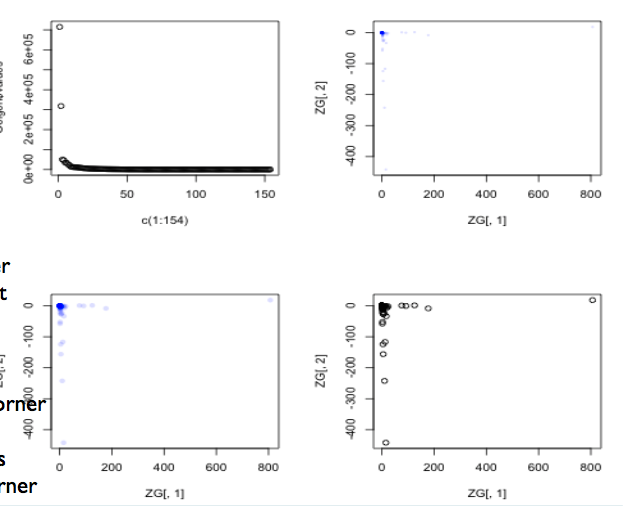
\includegraphics[scale=0.5]{enron.png}
\end{center}
\caption{Enron data}
\label{fig:enron}
\end{figure}


Are these results informative? In fact, employee 20 (Jeff Dasovich, the Legal Regulatory and Government Affairs Director, a senior employee) sent an extremely large numbers of emails to 4 or so people. This made him an outlider, which resulted in him dominate the first principal component due to his large $L^2$-norm. This illustrates that it is a good idea to remove outliers before performing PCA, since PCA assumes Gaussianity (by using the $L^2$-norm), which is easily swayed by outlying observations. Employee 57 (Tana Jones, the ENA Legal Specialist, a junior employee), also sent large numbers of emails to 4 or so people, but not as many as Jeff Dasovich. As a result, Tana Jones dominated the second principal component. 

The other outliers on the first principal component, we find that these are also legal employees who have sent relatively large numbers of emails to the same group of people (which explains why the show up along the same direction as the first component). Employees 3 (a VP) and 59 (a manager at West Power) received many emails from all three legal employees.

The second component contains a number of outliers, who again, sent many emails to a particular group of people.

What if we instead centered and scaled the data, we found much more meaningful rsults. We obtain one large eigenvalue and many smaller eigenvalues with no big gaps. Taking the top 5 components, we explain 32\% of the variability, whereas taking the top 10 principal components we explain 50\% of the variability. The top two principal components don't appear to be a good representation of the data. However, if we consider the data that we have, it might make sense that $L^2$ is not a meaningful metric to use; perhaps $L^1$ scaling makes more sense since we are dealing with count data...

\begin{figure}[H]
\begin{center}
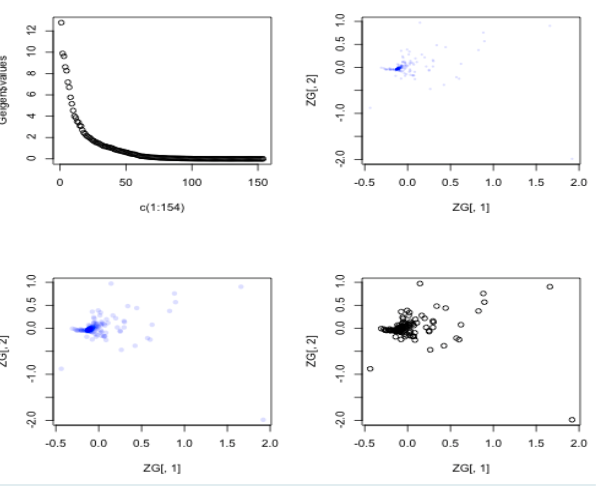
\includegraphics[scale=0.5]{enron2.png}
\end{center}
\caption{Enron data}
\label{fig:enron2}
\end{figure}


The outliers in the first component are employees 20, 37, 41, 61, 63, 65, 72 and 88 who do not share the same receivers of emails, moreover except for employee 20, the rest are all from trading or other departments. The outliers on the second component direction are employees 24, 37, 57, 63, 65 and 96, who are all from trading and other departments except for 57 whom we saw in our unscaled analysis.

The above PCA analyses are suggestive to give leads for further follow-up studes, however they are not conclusive in any sense! We note, however, that Employee 20 (Jeff Dasovich) and Employee 57 (Tana Jones) both appeared in news reports related to the Enron investigation.




\section{To normalize or not to normalize:}

As a rule of thumb, if you're not sure whether or not you should center and scale your data, do both and compare the results so that you can make a reasonable judgment call. However, in order to avoid one predictor having an undue influence on the principal components, it is common to first standardize the predictors to have mean zero and variance 1 before conducting PCA. Therefore PCA analysis has the following steps:

\begin{enumerate}
\item Center the predictors to have mean 0
\item Form the sample covariance matrix, $G$
\item Carry out an eigenvalue decomposition of $G$ to get eigenvalues $d_1 \geq ... \geq d_p \geq 0$ and the corresponding eigenvectors $U_j$
\item Keep all the large principal components that account for most of the variation in the data. For example, starting with 20 predictors it might be the case that the first 4 components account for $90\%$ of the total variation, i.e. the sum of the first 4 eigenvalues is about $90\%$ of the total sum of all eigenvalues.

\end{enumerate}

In the Enron study, we are looking for the outliers!


\section{PCA on the fruitfly project}

Recall that for the fruitfly project, we have a number of images of Drosophila embryos in each of which we have stained for certain genes. Since each embryo has a different size and shape, to make the embryos comparable, we must first find the outline of the embryo in the image and then warp it into a common ellipse as shown in the graphic below.

\begin{figure}[H]
\begin{center}
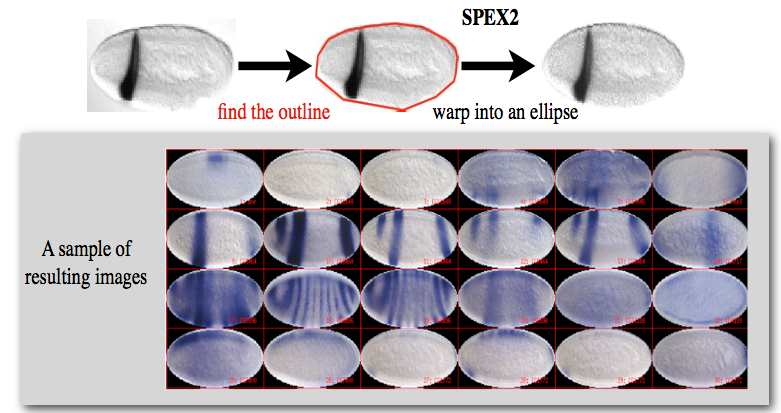
\includegraphics[scale=0.5]{fruitfly_ellipse.png}
\end{center}
\caption{Fruitfly ellipse}
\label{fig:fruitfly_ellipse}
\end{figure}


We then used PCA on the data from approximately 7 images to obtain the principal components shown below, where the colour of each component corresponds high intensity (red) and low intensity (blue).

\begin{figure}[H]
\begin{center}
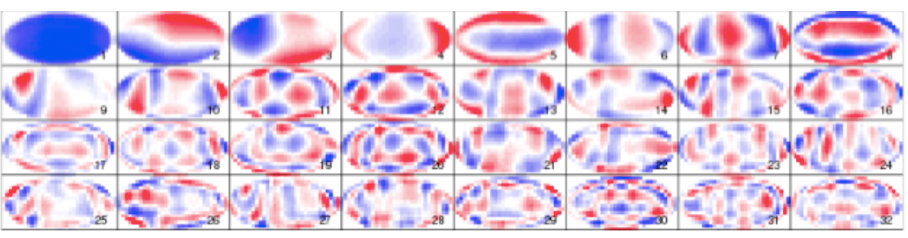
\includegraphics[scale=0.4]{pca_embryo.png}
\end{center}
\caption{PCA on the Fruitfly embryos}
\label{fig:fruitfly_pca}
\end{figure}




\section{Independent component analysis}
Unfortunately, the components identified by PCA for the fruitfly data didn't seem to be biologically interpretable. An alternative to PCA is Independent Component Analysis (ICA) which find the independent components by maximizing the independence of the estimated components by maximizing the non-Gaussianity. This has the effect of encouraging sparsity in the components. The resultant components for the fruitfly embryos using ICA are significantly better than those obtained by PCA. We are finding the biologically meaningful stripes and segments known by biologists.


\begin{figure}[H]
\begin{center}
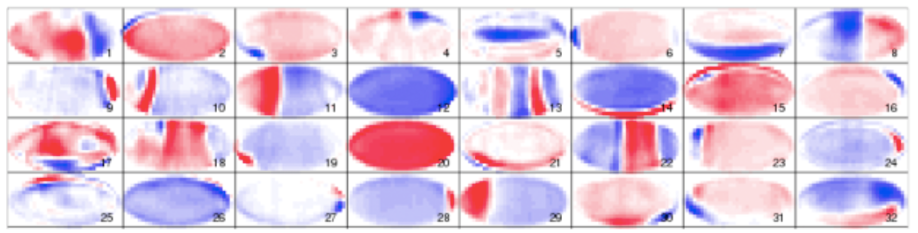
\includegraphics[scale=0.4]{ica_embryo.png}
\end{center}
\caption{ICA on the Fruitfly embryos}
\label{fig:fruitfly_ica}
\end{figure}

The reason that PCA doesn't work well is that it doesn't take advantage of the natural sparsity of the problem.

\section{Sparse PCA}

Regular principal component analysis typically finds linear combinations of all variables, which results in the disadvantage that the resultant components are often hard to interpret. Sparse PCA attempts to ameliorate this issue by finding linear combinations of just a few input variables.


\section{Non-negative matrix factorization}

We will discover that another alternative is non-negative matrix factorization


\section{A comparison of PCA, ICA and NMF}

We have introduced in this section several alternative (but related) approaches to the same problem: principal component analysis, independent component analysis and non-negative matrix factorization. Why do these different approaches exist? Well it turns out they all work best under different circumstances, although under which circumstance your data problem lies might be hard to identify. It might be an idea to try all three approaches on your dataset, and if you find that the results are different, then you will learn a lot by asking \emph{why} each method obtains different results. In fact, this is a good general rule for approaches with several possible methods, let's call it ``method stability''. If you are drawing a conclusion, you can gain confidence about the strength of the conclusion you're drawing if you can show that the results are robust to the specific method being used. In other words, conclusions are more believable if they hold when using many different analytical methods. This is a great way of showing that your conclusions are not simply an artifact of the method used. To compare results, it will be an even better idea to set aside a ``validation set'', say one third of your data, for ``independent'' comparison.




\chapter{Clustering}
\label{ch:clustering}


The basic idea behind clustering is that we want to find groups of similar observations in our dataset. The observations within these groups should "cluster together" more than with observations from other groups. The question is, how do we find these groups given that we have no idea even of the number of groups that exist in the dataset? First, we need to define some "distance" metric to describe how "far" different observations are from one another. Clustering is often called \emph{unsupervised learning}: unsupervised in the sense that we don't pre-define the groups so that our algorithms are not being "supervised" by these pre-existing classes, they much find their own! We will focus on some of the most common approaches to clustering such as K-means, PAM, hierarchical clustering, spectral clustering and the EM algorithm.

Clustering is very much related to network analysis which are extremely prominent in areas such as social network analysis: there are multitudes of researchers whose sole purpose in their professional or academic life (perhaps even in their entire life) is to find communities within social networks, such as those in the images below.


\begin{figure}[H]
\begin{center}
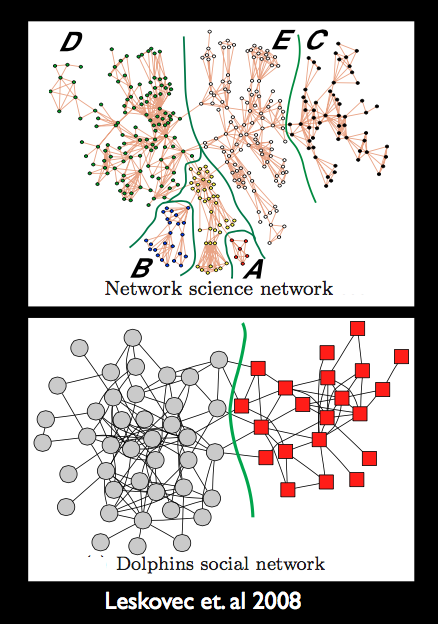
\includegraphics[scale=0.4]{network.png}
\end{center}
\caption{Network}
\label{fig:network}
\end{figure}

\section{K-means}


One of the most intuitive clustering algorithms is the K-means algorithm (often called the Lloyd-Max algorithm). The K-means algorithm finds $k\_c$ clusters (this number must be specified by the user) by first choosing $k\_c$ data points at random as the initial cluster centers (``centroids'') and subsequently assigning each data point to the cluster whose center it is closest to. Each centroid is then replaced by the mean of all data points assigned to that cluster, and the process is iterated until no data point is reassigned to a different cluster. The end result is a partition of the index set $\{1, ..., n\}$ into clusters $I_1, ..., I_{k_c}$ and cluster centers (or centroids), $C_1, ..., C_{k_c}$ that minimize the following global objective function (for any distance metric, $d$):

$$(C_1, ..., C_{k_c}) = \underset{(C_1, ..., C_{k_c})}{\text{argmax}} \sum_{i=1}^{k_c} \sum_{x_j : j \in I_i} d(x_j, C_i)$$

For example, if our distance metric is the regular $L^2$ norm, then this is simply

$$(C_1, ..., C_{k_c}) = \underset{(C_1, ..., C_{k_c})}{\text{argmax}} \sum_{i=1}^{k_c} \sum_{x_j : j \in I_i} (x_j - C_i)^2$$


\begin{figure}[H]
\begin{center}
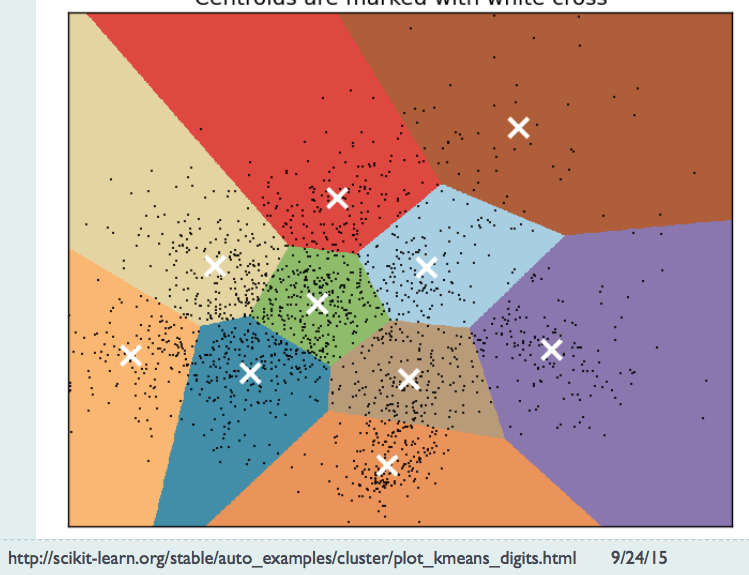
\includegraphics[scale=0.4]{kmeans.png}
\end{center}
\caption{K-means}
\label{fig:kmeans}
\end{figure}


The specific K-means algorithm can be described as follows:

\begin{enumerate}
\item The initial step: Specify $k_c$ initial cluster/group centers (for example by randomly selecting $k_c$ points without replacement from our $n$ observations).\\ Denote these centers as
$$C_1^0, ..., C_{k_c}^0$$
Then generate a partition of our observations (which we will identify by the index set $\{1, ..., n\}$) into non-overlapping subsets of the index set
$$I_1^0, ..., I_{k_c}^0$$
based on the following assignment rule: observation $i$ belongs to $I_k^0$ iff $i$ is closer to $C_k^0$ than all other centers in $d$-distance.
\item Determine new centers
$$C_1^1, ..., C_{k_c}^1$$
by find the point such that the sum of its distances to all other points in the corresponding clusters $I^0_0, ..., I^0_{k_c}$ is minimized. If $d$ is the usual Euclidean $L^2$-norm, then this corresponds to taking the mean of the points in a cluster to find the new center. If $d$ is the $L^1$ norm, then we are finding the median point.\\
Partition the observations into new clusters
$$I_0^1, ..., I_{k_c}^1$$
by the assignment rule from the previous point.
\item Repeat the above step by finding the centers of our new clusters, and then reclustering based on assignment rule for the new cluster centers.
\item Stop the process if two successive iterations lead to the same partition or when a stopping criterion is satisfied (for example, the decrease in within-groups variance falls below a certain threshold, or a preset maximum number of iterations is achieved).
\end{enumerate}







As an aside, suppose that we want to find $k$ unique clusters. We can re-write K-means in a more modern setting as follows

$$\hat{\mu} = \underset{M \in \mathcal{R}(n, k)}{\text{arg}~\text{min}} \| X - M\|_F^2$$

where $\| \cdot \|_F^2$ is the \emph{Frobenius norm}, (where for an $m \times n$ matrix $A$, $\|A\|_F = \sqrt{\sum_{i=1}^m \sum_{j=1}^n |a_{ij}|^2}$) and $\mathcal{R}(n, k)$ is the set of matrices with $k$ columns and $n$ rows, but only $k$ of these rows are \emph{unique}. The unique rows correspond to the $k$ centroid in the K-means objective function. This formulation allows for direct comparison with other optimization methods such as PCA. Note that
$$\underset{M \in \mathcal{R}(n,k)}{\min} \|X - M\|_F^2 = \underset{\{m_1, ..., m_k\} \subset \mathcal{R}^k} \sum_i \underset{g}{\min} \|x_i - m_g \|_2^2$$


To understand what the above formulation is saying: note that K-means aims to minimize the overall distance between the data and the centroids.





\section{PAM}

The Partitioning Around Medoids (PAM) clustering method (often called the K-medoids algorithm) is a modified version of K-means whereby it attempts to minimize the global sum of squares (as in K-means with the Euclidean $L^2$ metric), but subject to the constraint that the centers $C_1, ... C_{k_c}$ must be an actual data point (rather than just the average of data points, which may not itself be a data point). 

One way to minimize this constrained objective function is to modify the K-means or Lloyd-Max algorithm by first finding the mean location within the group (as per usual), and then replacing each center by the data point closest to it. 


\section{Hierarchical clustering}

To conduct hierarchical clustering, we begin with each observation being in its own lonely cluster. For example, we have $\{1\}, \{2\}, \{3\}, \{4\}$. Next, we find the two points that are the closest, and combine their clusters. So that, if the first an the second observations were the "closest" pair of points, our new partitioning is $\{1, 2\}, \{3\}, \{4\}$. We now have $n-1$ points to cluster. Let's repeat this process: find the next two closest points and aggregate their clusters. If the next smallest pairwise distance was between observations $1$ and $3$, then our new partitioning would be $\{1, 2, 3\}, \{4\}$, but if it were between observations $3$ and $4$, then our new partitioning would be $\{1, 2\}, \{3, 4\}$.

The idea is to continue this process until all observations are in a single cluster (which would require only one more step in the example above). This process generates a hierarchical clustering tree: at each level, we have a different number of clusters. We can choose to cut the tree at any point to get different numbers of clusters, and the number of clusters increases as the cut-point approaches the initial point.

This hierarchical representation is particular nice since it generates \emph{many} possible clusters: the result is a set of $n$ nested partitions containing anywhere from $1$ to $n$ clusters.

\section{Minimum spanning trees (MST)}

\section{Spectral clustering}

Recall our discussion on PCA. Luckily for you, spectral clustering, though it might seem scary at first, is essentially just PCA (the ``spectrum'' of a matrix refers to its eigenvalues) combined with K-means. The method actually is actually very prominently used in network analysis. To make life easier below, we will begin with some network notation. A network (or "graph"), $G$ consists of a \emph{vertex set} $V$ (for example, each vertex might correspond to a person or a gene) and an \emph{edge set}, $E$, which contains the set of edges between pairs of vertices (for example, there might be an edge between individual $1$ and $7$ because they are best friends, but there might not be an edge between individual $1$ and $3$ if they severely dislike one another). We often use the notation
$$G = (V, E)$$
to describe a network $G$. In community detection, what we're really trying to do is to find $k$ communities (subsets) of nodes (observations) in the graph such that the nodes within each cluster are more highly connected to one another than to the nodes in other clusters. We can define our a set of all possible $k$ communities, $\mathcal{C}_k$ to be
$$\mathcal{C}_k = \left\{ (C_1, C_2, ..., C_k) : \forall i \neq j, ~~ C_i \cap C_j = \emptyset, ~ ~ \bigcup_i C_i = V \right\}$$
which can be read as \emph{``the $k$ disjoint communities $C_1, C_2, ..., C_k$ that together, contain all of the nodes in $V$''}. But we still haven't described how to come up with these communities! One formulation is to find the $k$ communities which are defined such that they maximize some partition quality measure (a function that tells us how good out communities are at partitioning the data), $f_G$:

$$\underset{(C_1, ..., C_k) \in \mathcal{C}_k}{\text{arg}~\text{max}}f_G(C_1, ..., C_k)$$

So we've now formulated the problem, but how do we find a suitable measure $f_G$, especially since in most situations, this problem is NP-hard! We'll now describe the spectral clustering approach to this problem, and show that it is essentially PCA combined with K-means.

First, we need to translate the network into a matrix: let's use the symmetric \emph{adjacency matrix}, $W \in \mathbb{R}^{n \times n}$, whose entries 
$$W_{ij} = W_{ji} = \begin{cases} 1 & \text{if } (i, j) \in E \\ 0 & \text{otherwise} \end{cases}$$ 
represent whether or not there exists an edge between observation $i$ and observation $j$ in the network. We can also define the \emph{diagonal degree matrix}, $ D \in \mathbb{R}^{n \times }$, whose diagonal entries specify the degree (number of incident edges or connections) of each node:
$$D_{ii} = \sum_j W_{ij}$$


You might ask, why would we want to use an adjacency matrix? Surely we can define a more informative matrix, for example, instead of simply defining $W_{ij}$ to be $1$ when there is an edge between observations $i$ and $j$, why not let the value in the matrix reflect the \emph{strength} of the connection? For example, to link back to our discussions on Kernel functions, $K_h$ (an example might be the Gaussian density function), we could define the alternative matrix

$$W_{ij} = K_h(X_i - X_j)$$

where $X_i \in \mathbb{R}^p$ is a vector of the $p$ measured variables for observation $i$. There exist nice theoretical properties of such formulations, but in the discussion that follow we will proceed with a general adjacency matrix, $W$, defined in any way you like (if you prefer the simple $0-1$ adjacency matrix, that's just fine!). 

The next useful object is the \emph{Laplacian matrix}, typically defined by the symmetric graph Laplacian:
$$L_0 = D - W$$

However, just like our adjacency matrix, there are many different possible definitions of the Laplacian matrix, each of which normalize by degree (number of connections) in a slightly different way. For example, the \emph{random walk Laplacian}:
$$L_{rw} = I - D^{-1}W,$$

the \emph{normalized symmetric graph Laplacian}:
$$L_N = 1 - D^{-1/2}WD^{-1/2}$$

and the Laplacian that we will use which is a special version of the normalized symmetric graph Laplacian
$${\bf L = D^{-1/2}WD^{-1/2}}$$

Note that performing eigenvalue decomposition of $L$ and $L_N$ yield the same results! So why are we even interested in the Laplacian matrix? It turns out that the second eigenvalue of the normalized Laplacian (both the standard version and our version of it) is closely connected to the conductance of a graph (a measure of how ``well-knit'' the graph is) via Cheeger's inequality. Conductance controls how fast a random walk on the graph converges to a uniform distribution, but we won't worry too much about that here.

By this point you're probably sitting there wondering if we're ever going to get to spectral clustering itself. The answer is yes, we are, and here it is: suppose that we want to find $k$ clusters of observations


\begin{enumerate}
\item Input: Adjacency matrix $W \in \{0, 1\}^{n \times n}$, number of clusters $k$
\item Find the eigenvectors $X_1, ..., X_k \in \mathbb{R}^n$ corresponding to the $k$ largest eigenvalues of the Laplacian matrix $L$. $L$ is symmetric, so we can choose these eigenvectors to be orthogonal.
\item Form the eigenvector matrix $X = [X_1, ..., X_k] \in \mathbb{R}^{n \times k}$ whose columns correspond to the eigenvectors.
\item Treating each of the $n$ rows in $X$ as a point in $\mathbb{R}^k$, perform K-means. This creates $k$ non-overlapping sets $A_1, ..., A_k$ whose union is $1, ..., n$.
\item Output: $A_1, ..., A_k$. This means that node $i$ is assigned to cluster $g$ is the $i$th row of $X$ is assigned to $A_g$ in step 2.
\end{enumerate}




So really all spectral clustering does is a) PCA on the Laplacian matrix for dimensionality reduction, followed by b) K-means for clustering. So many modern methods that seem complex and fancy are really just concatenating more commonly used, "simpler" methods. It is much easier to build on the work of others than to start from scratch. In actuality, if all researchers ever did was come up with new novel methods and had no interest in extending and combining existing methods, we wouldn't get very far!

So given the above discussion, why did we do PCA and K-means? Why not do PCA and hierarchical clustering? Honestly, there's probably not a particularly good reason... we could certainly instead do hierarchical clustering instead of K-means, which is just the convention!


\begin{figure}[H]
\begin{center}
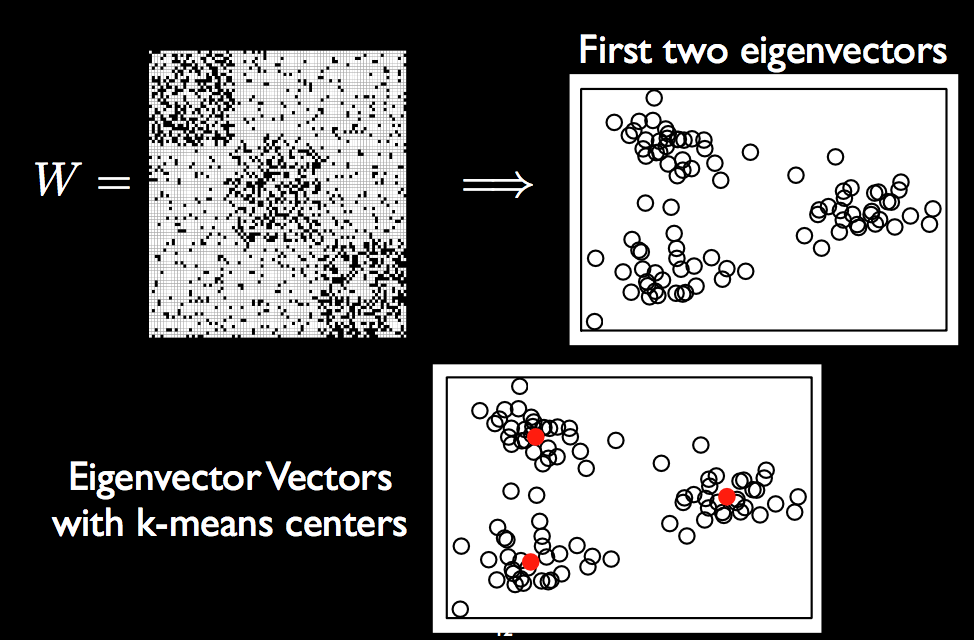
\includegraphics[scale=0.4]{spectral.png}
\end{center}
\caption{Spectral clustering}
\label{fig:spectral}
\end{figure}


Spectral clustering is adaptive to the intrinsic structure of the problem; it works well under a variety of different situations. 


\subsection*{Spectral clustering for directed graphs}

The above method does not make any mention of ``directed'' graphs. In particular, it makes no assumption on the direction of a relationship or connection between two nodes. Consider, for example, the Enron dataset. We can code this example as a network, where the 154 nodes are the employees of the company and the edges are the email communications between the employees. However, a single email is not two-directional: it is sent from one person and received by another. So rather than defining an edge by the presence of an email communication, we could define directed edges, whereby an edge points from employee $i$ to employee $j$ if an email was send from employee $i$ to employee $j$. In this way, the similarity matrix is no longer symmetric (since employee $j$ may not have send the same number of emails to employee $i$ as employee $i$ sent to employee $j$), and we can define it by:
$$A_{ij} = \text{the number of emails send from employee $i$ to employee $j$}$$
Similarly, the Laplacian matrix is asymmetric. Standard spectral clustering would produce complex (in the $i = \sqrt{-1}$ sense) eigenvectors on such a matrix, and existing works symmetrize the matrix and subsequently proceed by the usual spectral clustering approach. 

The method that we will describe below proposes and examines a specral clustering algorithm that replaces the eigen-decomposition with \textbf{singular value decomposition}, which can be performed on asymmetric matrices to produce left and right eigenvectors (in symmetric matrices, the left and right eigenvectos are equal and correspond to the usual eigenvectors). 

The adjacency matrix, $W \in \{0, 1\}^{n \times n}$ for a directed graph is \emph{asymmetric}:
$$W_{ij} = \begin{cases} 1 & \text{ if } i \rightarrow j\\ 0 & \text{ otherwise} \end{cases}$$

so that an entry in the adjacency matrix exists if there is an edge directed \emph{from} $i$ to $j$ but if there is no edge from $j$ to $i$ (even if there is an edge from $i$ to $j$), then $A_{ji} = 0$. Alternative, we could use a weighted adjacency matrix (where the entries are not simply 0 or 1, but they are 0 in the absence of an edge and nonzero in the presence of an edge), where if $i \rightarrow j$, we have $W_{ij} > 0$. Let's suppose for simplicity, however, that we have the standard $0-1$ adjacency matrix. We can define the number of "parents" (or in-links) of node $i$ as

$$P_{ii} = \sum_k W_{ki} = \sum_{k} 1\{k \rightarrow i\}$$

and the number of ``offspring'' (or out-links) of node $i$ to be
$$O_{ii} = \sum_k W_{ik} = \sum_k 1\{i \rightarrow k\}$$

These can be considered the directional generalizations of degree (number of \emph{directed} connections), and the Laplacian matrix to be

$$L_{ij} = \frac{W_{ij}}{\sqrt{O_{ii}P_{jj}}}$$


The new directed spectral clustering algorithm, \emph{DI-SIM} (pronounced ``Dice 'em'') can be described by

\begin{itemize}
\item Input: Adjacency matrix $W \in \{0, 1\}^{n \times n}$, number of clusters $k$
\item Compute the singular value decomposition of $L = U \Sigma V^T$. Remove the columns of $U$ and $V$ that correspond to the $n - k$ smallest singular values in $\Sigma$. Call the resulting matrices $U^k \in \mathbb{R}^{n \times k}$ and $V^k \in \mathbb{R}^{n \times k}$ 
\item Cluster the nodes based on similar parents by treating each row of $V^k$ as a point in $\mathbb{R}^k$. Cluster these points with K-means. Because each row of $V^k$ corresponds to a node in the graph, the resulting clusters are clusters of the nodes.
\item Cluster the nodes based on similar children by performing step two on the matrix $U^k$.
\item Output:the clusters from Steps 2 and 3.
\end{itemize}

The directed spectral clustering algorithm creates two sets of clusters.

\textcolor{red}{In 15-lec8.1 there is a description of SVD that I need to put in somewhere, probably in the PCA file}


\subsection*{Directed spectral clustering example on the Enron data:}

First, we computed the left and right singular vectors of the directed graph Laplacian. Suppose that we restrict to only the second, third, fourth and fifth vectors (see the image below), then we have two matrices with 154 rows and 4 columns: the left singular vectors $U \in \mathbb{R}^{154 \times 4}$ and the right singular vectors $V \in \mathbb{R}^{154 \times 4}$. Two rows in the matrix of left singular vectors are "close" if those two employees \emph{sent} many messages to the same people. Whereas two rows in the matrix of the right singular vectors are close if those two employees \emph{received} many messages from the sample people. 


\begin{figure}[H]
\begin{center}
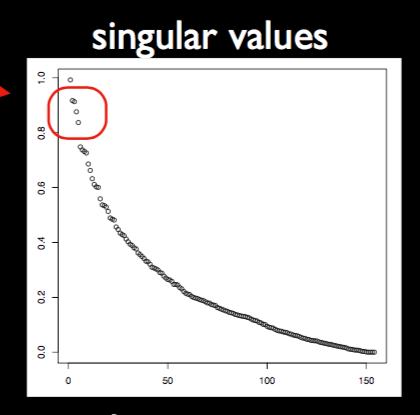
\includegraphics[scale=0.4]{singular.png}
\end{center}
\caption{Enron data}
\label{fig:Enron}
\end{figure}

The question is, how different (or similar) are the left and right singular vectors in the Enron data?

To compare the rows of $U$ to the rows of $V$, we need to make sure that they are "aligned". Recall that the matrix $O$ consists of the numbers of offspring/out-links for each node in the graph. If we define
$$O^* = \underset{O : O^TO = I}{\text{argmin}} \|U - VO\|_F$$
Then it becomes meaningful to measure the Euclidean distance between the rows of $U$ and the rows of $VO^*$, since $VO^*$ is aligned with $U$. The 154 distances are represented in the histogram below:



\begin{figure}[H]
\begin{center}
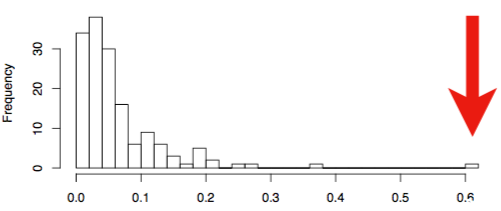
\includegraphics[scale=0.4]{dist.png}
\end{center}
\caption{Enron data distances}
\label{fig:dist}
\end{figure}


The outlier on the far-right corresponds to employee Bill Williams, who sent a lot of emails, but did not receive many. Note that Williams was not identified in the symmetric PCA analysis.

\section{The EM algorithm}

The expectation-maximization (EM) algorithm is an iterative algorithm which aims to compute the maximum likelihood estimate (whereby our goal is to estimate the model parameters for which the observed data are most likely) in the presence of missing or hidden data. It is related to techniques such as Newton-Rhapson and gradient descent. Each iteration consists of two steps: the E-step (expectation step) and the M-step (maximization step). In the E-step, the missing data (for example, the cluster membership) are estimated via a conditional expectation given the observed data and current estimate of the model parameters. In the M-step, the likelihood function is maximized under the assumption that the missing data are known, where the estimate of the missing data from the E-step are used in place of the actual missing data (since, obviously, this data is still missing!).

It is actually not hard to show that K-means in actually a variant of the EM algorithm. In the context of K-means, we might think of the E-step as the step which assigns each object to a centroid which corresponds to the most likely clustering, and the M-step as the recalculation of the model (recalculate the centroids using least squares optimization). 

The figure below from Dempster et al. (1977) provides a graphical interpretation of a single iteration of the EM algorithm.


\begin{figure}[H]
\begin{center}
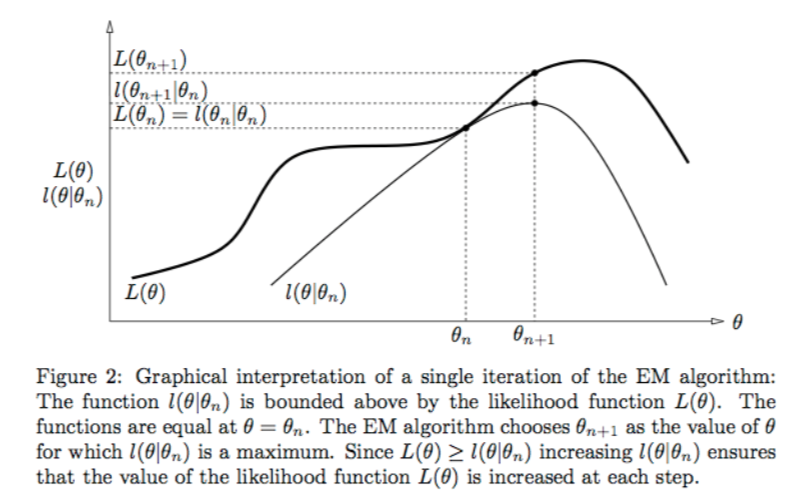
\includegraphics[scale=0.4]{EM.png}
\end{center}
\caption{The EM algorithm}
\label{fig:em}
\end{figure}

A clear and concise tutorial on the technical aspects of the EM algorithm is available by Sean Borman. We present only a concise summary here. Let's suppose that we have an unknown parameter, $\theta$, which indexes a distribution from which our observed data, $X$, was drawn. Suppose also that we have some missing data denoted by the hidden random vector, $Z$. As an example, suppose that our data, $X$, comes from a mixture of two Gaussians. In this case, each observation $X_i$ comes from one of two Gaussian distributions: $N(\mu_0, \sigma_0^2)$ or $N(\mu_1, \sigma_1^2)$ (in which case we assume that $\theta = (\mu_0, \sigma_0^2, \mu_1, \sigma_1^2)$), but the problem is that not only do we not know which distribution a given data point came from, we don't even know what the distributions are since $\theta$ is unknown! Can you imagine what our missing variable, $Z$, corresponds to? Well, given that the information that is missing is from which distribution our data was drawn, we might encode our latent variable to be
$$Z_i = \begin{cases} 1 &\text{if } X_i \sim N(\mu_1, \sigma_1^2)\\ 0 &\text{if } X_i \sim N(\mu_0, \sigma_0^2)\end{cases}$$

We can thus rewrite out distribution as

$$X|Z \sim ZN(\mu_1, \sigma_1^2) + (1 - Z) N(\mu_0, \sigma_0^2)$$

and stress that this is a significant abuse of notation, and that you should never write something like this (\emph{especially} not in a book!). 

That is, $Z_i$ is an unobserved random variable that tells us which distribution our observation $X_i$ came from. This is clearly a clustering problem! We observe a bunch of (normally distributed?) data points, for which we have reason to believe that there exist two main clusters of observations, and we would like to know what they are: we want to find $Z$! 

The idea is that, given a current estimate, $\theta_n$ of $\theta$ (where the subscript $n$ corresponds to the $n$th iteration, not the number of data points), we can iterate through the following steps:

\begin{enumerate}
\item Estimate the cluster membership, $z$, for the data point using conditional expectation given the observed values of the data point, $x$, and the current parameter estimates, $\theta_n$. That is, calculate $\hat{z}_n = E(z | x, \theta_n)$.
\item Calculate the value of $\theta_{n+1}$ that is most likely given $x$ and our estimated missing values (cluster membership), $\hat{z}_n$. This corresponds to calculating the maximum likelihood of $\theta$ at this iteration.
\end{enumerate}

Thus, as the EM algorithm converges (which it is guaranteed to do), not only does our estimate of $\theta$ get closer and closer to the ``true'' value, but the estimates of our cluster memberships (or missing values, $z$) get closer and closer to the true values. So our final cluster membership estimates corresponds to our final calculation of the E-step!

\textcolor{red}{Give some of the more technical details as well as an example}


\section{Two types of community detection algorithms: parametric and algorithmic}

There are two primary realms of community detection algorithms: 

\begin{enumerate}
\item Parametric model fitting approaches, and 
\item Algorithmic and data driven approaches.
\end{enumerate}

In the parametric model fitting approach, we suppose that a network model in which community memberships have a parametric representation. We aim to estimate these parameters which are considered the ``true'' clusters (recent examples include Nowicki and Snijders (2001), Handcock et al. (2007) and Airoldi et al. (2008). On the other hand, the algorithmic and data driven approach is motivated by observations, heuristics, and insights into the appearance of clusters. The user of such approaches hopes to find plausible clusters, but does not assume the existence of ``true'' clusters (recent examples involve spectral clustering, Girvan-Newman).


However, how do we know that we should ever trust the output of an algorithm? Many people tend to use the same methods over and over again because they found that the method worked well for them in the past. Is this ridiculous? Probably not that ridiculous... it might not be the absolute best method, but at least they've had success with it in some setting and have been working with the method for a long time and so hopefully have a fairly thorough understanding of the method. In general, however, it is very important to perform ``down-stream'' validation analysis to assess the empirical performance of a method. What do we mean by ``down-stream'' analysis? First, perhaps, we should ask the question: how do you know that the clusters you've obtained from your method of choice are meaningful? Typically we don't know the true clusters (if there even are true clusters...), and if we did, we would have no need to estimate the clusters in the first place! 

The typical computer-science approach to such questions is to show that particular algorithms yield approximate solutions that are ``close'' to the true empirical optimum for a particular set of network data. However, just because the algorithm has the capabilities to attain ``close to optimal'' solutions, how do you know that it has done so for your data? 

In contrast, the statistical approach asks: how does the algorithm perform on tractable stochastic models with clearly defined population clusters? Do we get close to the truth (that we build into the model)? To understand what this means, we first need to define the Stochastic Block Model (SBM). In an SBM, each node belongs to a ``block'', edges are randomly placed between nodes based on independent Bernoulli random variables and the probability of an edge between two nodes depends only on the block membership of those two nodes. In particular, we can think of the blocks as the ``true'' clusters and make the probability of an edge high between nodes in the same block and the probability of an edge low between nodes in different blocks. 



\begin{figure}[H]
\begin{center}
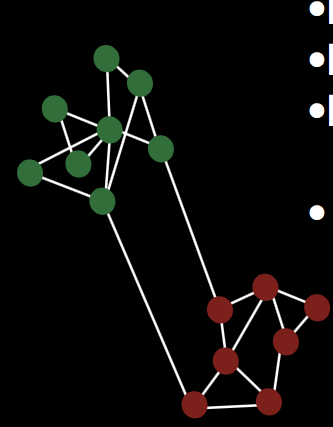
\includegraphics[scale=0.4]{SBM.png}
\end{center}
\caption{SBM}
\label{fig:sbm}
\end{figure}


If we can show that a clustering algorithm can accurately detect these blocks (the clustering algorithm estimates the block membership for each node) then we should be fairly confident that the algorithm performs well. But is this enough to be sure that the algorithm performs well in all circumstances?


\section{How to choose the number of clusters?}

So in all of the examples presented above, we have always assumed that we are trying to identify $k$ clusters, and we treated this number as something that you should just know! But this wasn't really fair... in most situations, we don't know how many clusters there are in our data. So how can we figure out the right value of $k$? There are a number of methods out there, but methods for which you simply plug in your data and it spits out a number of clusters are unreliable. A much better alternative is to visualize your data, and there are a number of tools available for the specific purpose of identifying the most appropriate number of clusters in your data. One such method is the Sihlouette plot.

\subsection*{Silhouette}

Silhouette was first introduced by Peter J. Rousseeuw in 1986. Assume that we have clustered our data into $k$ groups, and for any given data point, $i$, we define:


\begin{itemize}
\item $a_i$ to be a measure of how well observation $i$ fits into its cluster (for example by calculating the average pairwise distance of points in cluster $i$).
\item $b_i$ to be a measure of how different observation $i$ is from other clusters (for example by calculating the smallest average distance of observation $i$ to other clusters).
\end{itemize}


Then we can define a value, called the \emph{silhouette width} to be

$$s_i = \frac{b_i - a_i}{\max(b_i, a_i)}$$

which is a value between -1 and 1. In particular, $s_i$ is close to $1$ if observation $i$ is in a tight cluster and is far away from other clusters, and is close to $-1$ if it is in a loose cluster and is close to other clusters. Our goal is to find the value of $k$ that maximizes the mean of the $s_i$'s.

Since humans like to visualize things, we can use the Silhouette plot (plot the $s_i$'s in decreasing order for each cluster), and note that we want to see many large $s_i$ values. Below, we plot a Silhouette for an example with two clusters and compare when we instead used three clusters.


\begin{figure}[H]
\begin{center}
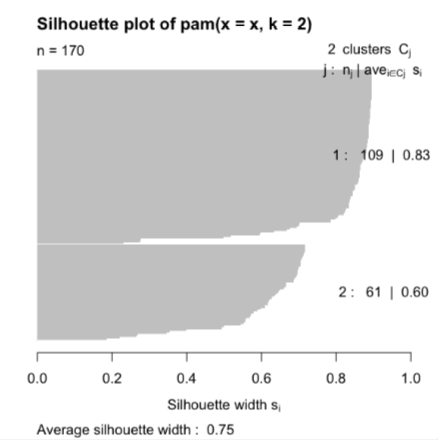
\includegraphics[scale=0.4]{silhouette2.png}
\end{center}
\caption{Silhouette with two clusters}
\label{fig:sil2}
\end{figure}



\begin{figure}[H]
\begin{center}
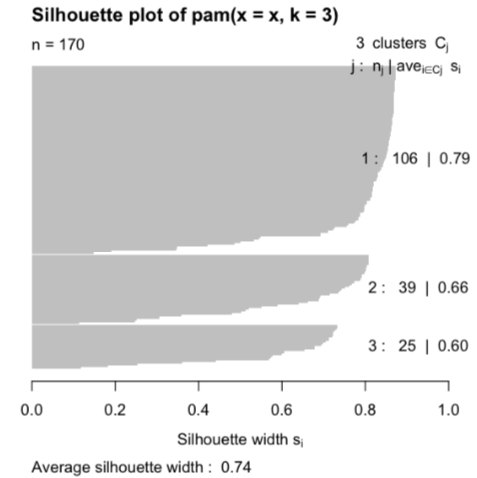
\includegraphics[scale=0.4]{silhouette3.png}
\end{center}
\caption{Silhouette with three clusters}
\label{fig:sil3}
\end{figure}



We see that the average silhouette width (the average $s_i$ values) remains approximately the same at 0.75 with two clusters and 0.74 with three clusters. However, since there appears to be no major difference in the quality of the clustering, since we encourage simplicity, we would prefer to use the two-cluster result.


\subsection*{Silhouette with the Enron data}

Below, we present Silhouette plots of 3- and 4-clusters from the Enron email data.


\begin{figure}[H]
\begin{center}
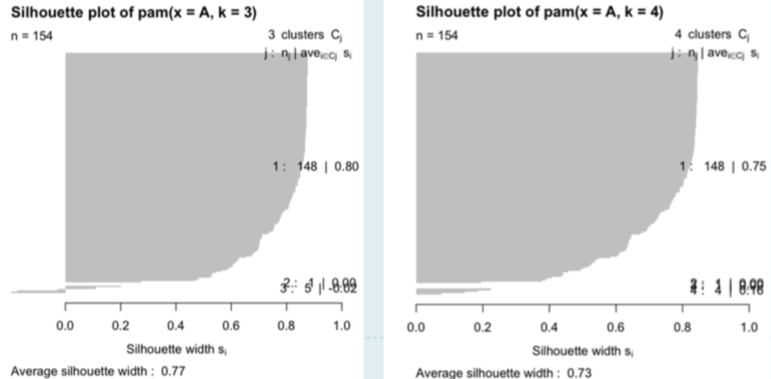
\includegraphics[scale=0.4]{enron_silhouette.png}
\end{center}
\caption{Silhouette for Enron data}
\label{fig:sil_enron}
\end{figure}

It is clear from the Silhouette plot that there is one extremely large cluster and the other clusters in both cases are very small and consist of only a few people (we note that these small clusters correspond to the lawyers in the company that we saw earlier in our discussion of PCA, for example employees 20 and 57). The average silhouette width is slightly smaller at 0.73 when we have 4 clusters than the average width of 0.77 when we have 3 clusters. In this situation, we must make a judgment call as to whether we prefer 3 or 4 clusters, however we concede that given the small difference it probably doesn't matter which one we choose.


\section{Cross-validation}

We have seen cross-validation several times already, but here we present another use for it. The idea is that we want to find the number of clusters for which we can minimize some objective function over different subsets of the data. The basic idea behind $V$-fold cross validation is to


\begin{enumerate}
\item Divide the data into $V$ batches
\item Given $k$, the number of clusters, remove the batches one by one and at each instance use the other $V-1$ batches to cluster by K-means
\item Calculate the K-means objective function value on the removed batch 
\item After performing the above steps on each of the $V$ batches, add up the $V$ objective function values and find the value of $k$ that yielded the smallest final value.
\end{enumerate}






\part{Regression}



\chapter{Linear models}
\label{ch:linear}


Suppose that we were interested in predicting height using measurements of weight as a predictor. A simple way to do this might be to come up with an equation of the form
$$\text{height} = a + b \times \text{weight}$$
for some constants $a$ and $b$. You might be revolted at such a gross oversimplification of the relationship between height and weight: surely we all \emph{know} that measurements height and weight don't fall on a perfectly straight line; there are all sorts of deviations! If you took the time to take a random sample of people, measure their heights and weights, and then plotted the height measurements against the weight measurements, you'll notice that there certainly are deviations from the straight line, but that the overall trend is linear. Thus, perhaps our model above will be more accurate if we add a term that can represent these deviations:

$$\text{height} = a + b \times \text{weight} + \epsilon$$

where $\epsilon$ is some random number that, on average is zero, but varies randomly about zero. A representation such as this is what we call a simple linear model: linear models can be used to describe a continuous response variable in terms of a linear combination of one or more predictor variables plus some noise. 

We can start to get fancy by adding other variables such as gender and age, and even perhaps some interaction terms, but we might be getting ahead of ourselves. There is an important question to ask first. What are the values of $a$ and $b$? The answer is, unfortunately, that we can never know. If this model is to be believed, these values exist for an overall population which is most likely so large that we can never measure the height and weight of every individual in the population. We can, however, observe a sample from this population, and we can use these sample individuals to \emph{estimate} the values of $a$ and $b$.

To motivate some notation, suppose that we want to fit a linear model to a response $y$ and we have $p$ predictor variables, $x_1, x_2,..., x_p$ then we can write this linear model as

$$y_i = \beta_0 + \beta_1x_{1,i} + \beta_2 x_{2,i} + ... + \beta_px_{p,i} + \epsilon_i$$

where the subscript $i$ specifies that we are talking about the model for individual $i$ from our sample. Notice that every individual has the same values of $\beta_1$, ..., $\beta_p$ (since these don't depend on $i$), but different values for $y_i, x_{1, i}, x_{2, i}, ..., x_{p, i}, \epsilon_i$. To frame this in the setting of the example above, each individual has different weights, ages, genders, etc but the same linear relationship exists between height and these predictor variables for each individual. 

Suppose that we have a sample of $n$ individuals from a population. We can write the above model in {\bf matrix form} as follows

$$Y = X \beta + \epsilon$$

where 

$$Y =\left[ \begin{array}{c}y_1\\ y_2 \\   \vdots\\   y_n\end{array} \right]$$ 

is a $n \times 1$ {\bf response vector} for our $n$ individuals, 

$$X =\left[ \begin{array}{ccccc}
1 & x_{1, 1} & x_{1, 2} & \dots & x_{1, p}\\
1 & x_{2, 1} & x_{2, 2} & \dots & x_{2, p}\\
\vdots &  \vdots & \vdots & \ddots & \vdots \\
 1 & x_{n, 1} & x_{n, 2} & \dots & x_{n, p} \end{array}\right]$$


is a $n \times (p + 1)$ {\bf design matrix} for our $n$ observations (the first column corresponds to the intercept term and the remaining columns correspond to the $p$ variable measurements for each individual),

$$\beta = \left[ \begin{array}{c}\beta_0 \\ \beta_1\\ \beta_2 \\   \vdots\\   \beta_p\end{array} \right]$$ 

is our $(p \times 1) \times 1$ {\bf coefficient vector}, and

$$\epsilon = \left[ \begin{array}{c}\epsilon_1\\ \epsilon_2 \\   \vdots\\   \epsilon_n\end{array} \right]$$

is our random $n \times 1$ {\bf error vector}, whose entries specify the deviations of each individuals response from the specified linear form. We typically assume that $E(\epsilon | X) = 0$ and $Var(\epsilon | X) = \sigma^2 I$, but we do not necessarily \emph{need} normality. As a result of these assumptions, we have that the expected response is given by

$$E(Y | X) = E(X \beta + \epsilon | X) = E(X \beta| X) + E(\epsilon | X) = X \beta$$

The model, $Y = X \beta + \epsilon$ is commonly referred to as a \textit{linear regression} model. However, recall that both $\beta$ and $\epsilon$ are unknown! If we knew $\beta$, we could make predictions of the form $\hat{Y} = X\beta$. Thus, to make a linear regression model useful, we need to \textit{estimate} the parameters, $\beta$. To recap, the primary assumptions underlying the linear regression model (beside from the obvious assumption of linearity) are


\begin{itemize}
\item The errors $\epsilon_i$ are independent and identically distributed (iid) with mean 0 and variance $\sigma^2$.
\item If the $X$ are random, we assume that $\epsilon$ is independent of $X$.
\end{itemize}


Note that nowhere have we explicitly assumed a Gaussian distribution for the errors!


\section{Fitting a linear model using OLS}


How do we come up with an estimator $\hat{\beta}$ of the population coefficients $\beta$? In general, we want to find the value of $\hat{\beta}$ such that the predicted $Y$ values, $\hat{Y} = X \hat{\beta}$ are as close to the true values, $Y$, as possible. If we use the $L^2$ measure of ``closeness'', then we want to find the value of $\beta$ that minimizes the quadratic loss function:

$$\hat{\beta} = \underset{\beta}{\text{arg}~\text{min}} \| Y - X \beta\|_2^2 =  \underset{\beta}{\text{arg}~\text{min}} \sum_{i = 1}^n (y_i - X_i \beta)^2$$

where $X_i = [1 ~ x_{i,1}~ x_{i, 2} ~... ~x_{i, p}]$ is the $i$th row of the design matrix (the predictor vector for observation $i$). In the image below, this corresponds to finding the line such that the vertical distances between the observations and the line are minimized.

\begin{figure}[H]
\begin{center}
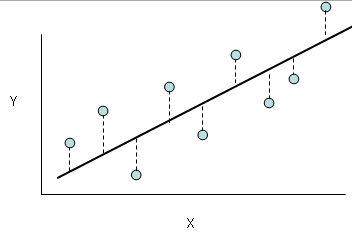
\includegraphics[scale=0.8]{OLS.png}
\end{center}
\caption{OLS}
\label{fig:ols}
\end{figure}

If our design matrix, $X$, is full rank, then the value of $\beta$ that minimizes the above expression can be written as 
$$\hat{\beta}_{OLS} = \left(X^TX\right)^{-1}X^T Y $$

and this is what we call the {\bf ordinary least squares} (OLS) estimator (because it is the minimizer of the \textit{squared loss} function). Note that if $X$ is not full rank, it is possible to calculate a generalized inverse using singular value decomposition, however in this case, the solution (the minimizer) is not unique, as we will explore below. 


\subsection*{The hat matrix: generating predictions}

In summary if we use OLS to estimate, $\beta$, the equation that we get (and thus the predictions from the linear model that we obtain) can be given by

$$\hat{Y} = X\hat{\beta}_{OLS} = X\left(X^TX\right)^{-1}X^TY = HY$$

where $H$ is called the {\bf hat matrix} (a cute name that arose due to the fact that $H$ puts a ``hat'' on Y). To be more technical, the hat matrix, $H$, is a projection matrix onto the linear space spanned by the columns of $X$. Note that $X$ is a matrix, so try your hardest to resist the temptation to cancel the $X$'s in the above expression (we cannot rearrange matrices like we can scalars: $ X\left(X^TX\right)^{-1}X^T \neq  \left(X^TX\right)^{-1}X^TX = I$).


A projection-based proof of the OLS formulation of $\hat{\beta}$ is as follows:

The idea is to use the hat matrix, $H = X(X^TX)^{-1}X^T$, to show that $HY$ is the projection of $Y$ onto the column space of $X$. To begin, it is straightforward to check that 

\begin{enumerate}
\item $H$ is idempotent: $HH = H$,
\item and thus that $(I - H)H = 0$, and
\item $X$ is invariant under $H$: $HXb = Xb$ for any $b \in \mathbb{R}^n$. 
\end{enumerate}


To show that $H$ is the projection matrix onto the column space of $X$, we can thus proceed as follows:

\begin{align*}
\|Y - X\beta\|_2^2 & = \|Y - HY + HY - X\beta\|_2^2\\
& = \|Y - HY + H(Y - X\beta)\|_2^2 && \text{from (3)}\\
& = \|Y - HY \|_2^2 + \|H(Y - X\beta)\|_2^2 + 2Y^T(I - H)H(Y-X\beta)\\
& = \|Y - HY \|_2^2 + \|H(Y - X\beta)\|_2^2 && \text{from (2)}\\
& \geq \|Y - HY\|_2^2
\end{align*}

This implies that the ($L^2$) distance from our response $Y$ to the ``true'' regression line, $X\beta$ is greater or equal to the distance from our response $Y$ to $HY$. Thus, since $HY = X(X^TX)^{-1}X^TY = X\hat{\beta}_{OLS}$, it must follow that this fitted line is the best that we can do in terms of estimating the line $X\beta$ by minimizing the distance between the fitted line and our response $Y$.

\section{Sources of randomness}

Let's ask a question: is $\hat{\beta}$ random? What about $\beta$? To answer this question, let's ask, where does the randomness in the model come from? We usually consider $X$ to be fixed (but this is not a requirement), and $\beta$ is a \textit{constant} (but unobservable) population variable. {\bf The only source of randomness in the regression model $Y = X \beta + \epsilon$ is in the random error, $\epsilon$} ($Y$ is random only because it depends on $\epsilon$). Keep this in mind, because it is very important! So we ask again: is $\hat{\beta}$ random? Look again at the formula $\hat{\beta} = \left(X^TX\right)^{-1}X^T Y$. The $X$ matrices are fixed, but $Y$ is random (due to its dependency on $\epsilon$). Thus, the answer is: yes, $\hat{\beta}$ is random! In fact, if we were to draw another sample and re-estimate $\beta$ using the new $X^*$ and $Y^*$, then we would get a different value for our estimator $\hat{\beta}^* = \left(X^{*T}X^*\right)^{-1}X^{*T} Y^*$ despite the fact that both $\hat{\beta}$ and $\hat{\beta}^*$ estimates of $\beta$: they can both be considered as realizations of the same {\bf random variable}, $\hat{\beta}$. 



\section{Residuals}


We can rearrange the above equation as

$$Y = X \hat{\beta}_{OLS} + e$$

where $e = Y - X \hat{\beta}_{OLS}$ are called the {\bf residuals}. The $i$th residual, $e_i$, measures how far the predicted response $\hat{y}_i$ is from the true value, $y_i$. However, it is a common misconception that the formula presented above is the regression model. This merely represents a relationship that is always true: that the observed values are equal to the predicted values plus the residuals (the difference between the observed and predicted values). There is no description in the above formula of the sources of randomness assumed by the model. The linear regression model is the formula containing the explicit random error variable $\epsilon$, $Y = X \beta + \epsilon$.

It is not hard to show that the vector of residuals, $e$, is orthogonal to $X$:

\begin{align*}
X^Te &= X^T(y - X\hat{\beta}) \\
& = X^T(y - X(X^TX)^{-1}X^Ty)\\
& = X^Ty - X^TX(X^TX)^{-1}X^Ty\\
& = X^Ty - X^Ty\\
&= 0
\end{align*}

moreover, this implies that the residuals always sum equal to zero \textit{whenever the model has an intercept term}. This is because the if the model has an intercept term, then the first column of $X$ is simply a column of $1$'s, and the orthogonality of $X$ and $e$ implies that

$$\sum_{i=1}^n e_i = 0$$

(if you're not sure where this came from, expand the matrix multiplication $X^Te$, and it should be clear).


Next, given that we have a {\bf fitted linear model}, $\hat{Y} = X \hat{\beta}$, how can we figure out how well the model is fitting the data? It makes sense to look at how close the fitted/predicted values are to the true values: that is, it makes sense to look at the residuals. In fact, a common measure of adequacy of model fit is given by the residual sum of squares (RSS):

$$RSS = \sum_{i=1}^n (y_i - \hat{y}_i)^2 = \sum_{i=1}^n e_i^2$$


However, looking at the $RSS$, we only get an overall view of how close the responses predicted by the model are to the true responses. Looking at the $RSS$ (or an $R^2$ value) and claiming that the model fits well is the equivalent of claiming to understand a dataset because we have looked at some summary statistics such as the mean of each variable. Clearly there is a lot more that we could consider! One such way is to assess the distribution of the residuals, usually though a plot of the residuals $e_i = y_i - x_i^T \hat{\beta}$ versus the fitted values $\hat{y}_i = x_i^T\hat{\beta}$ (although we could alternatively plot the residuals versus some other value such as time or a variable in the data).  In general, we hope to observe that the residuals are randomly scattered about the line $e = 0$, such as in the figure below.



\begin{figure}[H]
\begin{center}
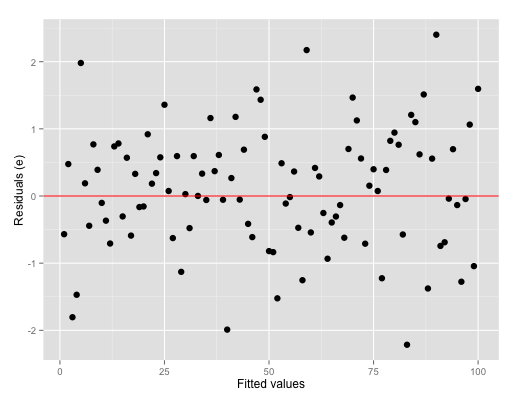
\includegraphics[scale=0.4]{residuals.png}
\end{center}
\caption{residuals}
\label{fig:residuals}
\end{figure}

On the other hand, patterns in the plot that do not follow this random scattering pattern are typically indicative of regions in the data where the model doesn't work well, or over-fits. For example, panel (a) in the figure below displays an example in which the variance of the residuals is much larger for large values of the fitted values. Such a residual plot can be used to identify heteroskedasticity (i.e. that our assumption of equal variance for all of our error terms was incorrect). In this case, we might decide that our original model was incorrect, and we are better off estimating $\beta$ using generalized least squares. The residuals in panel (b), however, exhibit extremely small variation, indicating that the model may be overfitting the data and thus is unlikely to work well on external datasets. One thing to keep in mind is the importance of the scale of the axis. In particular, if we zoomed in on the residual plot in panel (b), we would see an image resembling the randomly scattered residuals in the figure above. The interpretation of the plot depends on the scale used, so it is vital to use a scale appropriate to the data.


\begin{figure}[H]
\begin{center}
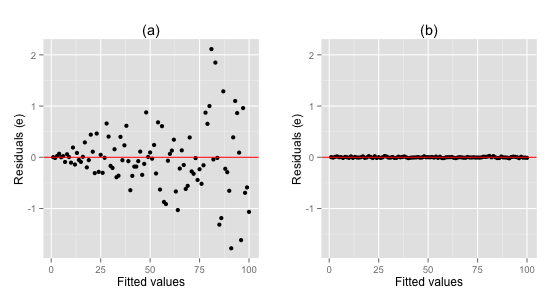
\includegraphics[scale=0.4]{badresiduals.png}
\end{center}
\caption{bad residuals}
\label{fig:badresiduals}
\end{figure}

Residual plots can be used to identify places where the model does not work well or over-fits. In particular, if the residuals appear to be randomly scattered about zero for a particular range of fitted values, but appear non-random for a different range of fitted values, we might conclude that the model is works well over the first range but not on the second.


%
\section{Properties of the OLS estimator $\hat{\beta}$}

Note that OLS was just one approach (in particular, minimizing the squared, or $L^2$, loss: $\sum_{i=1}^n(Y_i - X_i \beta)^2$) to estimating the coefficient vector, $\beta$. There are a number of alternative approaches such as the least absolute difference (LAD) which minimizes the $L^1$-loss $\sum_{i=1}^n|Y_i - X_i \beta|$ (we will discuss alternatives later). However, there are a number of properties that the OLS approach possesses that makes it particularly attractive as an estimator. Namely, the OLS estimator is unbiased and has an asymptotic Gaussian distribution. We will explore these properties below.


\subsection*{Unbiasedness}

It is not hard to show that the OLS estimator, $\hat{\beta}_{OLS}$, is \textit{unbiased}. That is, on average, over random samples from our population, our estimate, $\hat{\beta}_{OLS}$, will be equal to the ``true'' population value, $\beta$:

\begin{align*}
E\left(\hat{\beta}_{OLS} \Big| X\right) &= E\left( (X^TX)^{-1}X^TY \Big| X \right)\\
& = (X^TX)^{-1}X^T E(Y | X)\\
& = (X^TX)^{-1}X^T X\beta\\
& = \beta
\end{align*}

\subsection*{Variance}

Recall that the only source of randomness in the linear model is the random error, $\epsilon$. In particular, we assumed that the $\epsilon_i$ were iid with variance $\sigma^2$. This implies that the variance-covariance matrix of the vector $\epsilon = (\epsilon_1, ..., \epsilon_n)$ is given by
$$Cov(\epsilon | X) = \sigma^2 I _{n \times n} = \left[ \begin{array}{cccc} \sigma^2 & 0 & \dots & 0\\
0 & \sigma^2 & \dots & 0 \\
\vdots & \vdots & \ddots & \vdots \\
0 & 0 & \dots & \sigma^2 \end{array} \right]$$
The variance-covariance matrix of the OLS estimator, $\hat{\beta}_{OLS}$, is given by:

\begin{align*}
Cov\left( \hat{\beta}_{OLS} \Big| X \right) & = Cov\left( (X^TX)^{-1}X^TY \Big| X \right)\\
& = (X^TX)^{-1}X^T ~Cov(Y | X)~ X(X^TX)^{-1}\\
& = (X^TX)^{-1}X^T ~Cov(X\beta + \epsilon | X)~ X(X^TX)^{-1}\\
& = (X^TX)^{-1}X^T ~Cov(\epsilon | X)~ X(X^TX)^{-1}\\
& = (X^TX)^{-1}X^T~\sigma^2 I_{n \times n}~X(X^TX)^{-1}\\
& = (X^TX)^{-1}\sigma^2
\end{align*}


\subsection*{Example}
For a simple example, suppose that we have a simple linear model $y_i = \beta_0 + \beta x_i + \epsilon_i$, then 
$$X = [1 ~~~ x] = \left[ \begin{array}{cc} 1 & x_1\\ 1 & x_2 \\ \vdots & \vdots \\ 1 & x_n \end{array}\right]$$

which implies that 
$$(X^TX)^{-1} = \frac{1}{\sum_{i=1}^n x_i^2 - \left( \sum_{i=1}^n x_i\right)^2}\left[ \begin{array}{cc} \frac{1}{n} \sum_{i=1}^n x_i^2 & - \bar{x}\\ - \bar{x} & 1 \end{array} \right]$$

so our estimate is given by

$$\hat{\beta} = (X^TX)^{-1}X^Ty = \left[\bar{y} - \frac{Cov(x, y)}{Var(x)} \bar{x}~,~~ \frac{Cov(x, y)}{Var(x)} \right].$$


From here, it is easy to calculate the variance of $\hat{\beta}_0$ and $\hat{\beta}_1$:
$$Var(\hat{\beta}_0) = \sigma^2\frac{\frac{1}{n} \sum_{i=1}^n x_i^2}{\sum_{i=1}^n x_i^2 - \left( \sum_{i=1}^n x_i\right)^2},$$

and

$$Var(\hat{\beta}_1) = \sigma^2\frac{1}{\sum_{i=1}^n x_i^2 - \left( \sum_{i=1}^n x_i\right)^2}.$$



\subsection*{Asymptotic normality}

Since the OLS estimate of $\beta$ corresponds to the \textit{maximum likelihood estimate}, theoretical results tell us that when we have a large sample size, the distribution of our estimator, $\hat{\beta}$ should be approximately Gaussian. What should the mean and variance of this distribution be? We found the mean and variance of $\hat{\beta}$ above, so our distributional result is

$$\hat{\beta}_{OLS} \overset{n \rightarrow \infty}{\sim} N\left( \beta, \sigma^2 (X^TX)^{-1} \right)$$


In fact this asymptotic result follows from the {\bf central limit theorem} (CLT) which tells us that if we have a sequence of iid random variables, $X_1, ..., X_n$, drawn from \textit{any distribution}, and if $E(X_i) = \mu$ and $Var(X_i) = \sigma^2 < \infty$ for each $i$, then the distribution of the sample average, $\bar{X} = \frac{1}{n}\sum_{i=1}^n X_i$, tends to a normal distribution. More specifically, the result tells us that 

$$ \bar{X} \overset{d}{\rightarrow} N\left(\mu, \frac{\sigma^2}{n}\right)$$

which is quite remarkable, given that our sample of $X_i$'s could have come from any distribution at all (we just need the samples to be iid)! Most existing proofs of this fact are fairly tedious and fail to lead to an improved sense of intuition. An outline of the more interesting and intuitive proofs are discussed in an enlightening blog post by Terence Tao.



\subsection*{Estimating $\sigma^2$}

Note that the variance of $\hat{\beta}_{OLS} = \sigma^2 (X^TX)^{-1}$ depends on $\sigma^2$, the common variance of $\epsilon_i$. If we want to get an idea of how variable our estimate, $\hat{\beta}_{OLS}$ is, then it is important that we have some idea of what $\sigma^2$ is equal to. Unfortunately, we rarely do! Thus we need to estimate $\sigma^2$ somehow. As a first approach, perhaps we could estimate $\sigma^2$ by looking, not at the variance of $\epsilon_i$ (since these are unobserved), but rather at the variance of the residuals, $e_i$, which can be thought of as realizations of the error terms $\epsilon_i$ (in fact, they would be realizations of $\epsilon$ if the proposed linear model was the ``truth''). Recall that

\begin{align*}
e &= Y - HY = (I - H)Y\\
& = (I- H)(X\beta + \epsilon)\\
& = (I - H) \epsilon
\end{align*}

Then perhaps, since $\sigma^2 = Var(\epsilon_i) = E(\epsilon_i^2) \approx \frac{\sum_{i=1}^n e_i^2}{n}$, a reasonable estimate might be

$$\hat{\sigma}^2 = \frac{\|e\|_2^2}{n} = \frac{\sum_{i=1}^n e_i^2}{n}$$


This estimator, though not far from what we are searching for, turns out to be biased:

\begin{align*}
E\left[ ||e||^2 \Big| X \right] & = E \left[ ||(I - H) \epsilon||^2 \Big | X\right]\\
& = E\left[ \epsilon^T (I - H) \epsilon \Big| X\right] && (I - H)^2 = I - H \text{ and } ||a||^2 = a^Ta\\
& = E \left[ tr(\epsilon^T(I - H) \epsilon )\Big| X \right] && tr(a) = a \text{ for }a \in \mathbb{R} \\
& = E\left[ tr((I - H) \epsilon \epsilon^T) \Big| X \right] && tr(AB) = tr(BA)\\
& = tr\left( E\left[(I - H) \epsilon \epsilon^T \Big| X \right]\right)\\
& = tr\left((I - H) E\left[\epsilon \epsilon^T \Big| X \right]\right)\\
& = tr\left((I - H) Cov( \epsilon) \right)\\
& = \sigma^2 tr(I - H)\\
& = \sigma^2 (n  -p) &&\text{(trace of a proj. matrix is its rank)}
\end{align*}

Thus an unbiased estimate of $\sigma^2$ is given by

$$\hat{\sigma}^2 = \frac{\sum_{i=1}^ne_i^2}{n-p}$$


%
\section{Interpreting the linear model}

Suppose that we have a linear model

$$y = \beta_1 x_1 + \beta_2 x_2$$

and that we have estimated $\hat{\beta}_1 = 2$ and $\hat{\beta}_2 = 2.1$. How would we identify which predictor, $x_1$ or $x_2$, is ``important'' or ``suggestive'' of the response $y$? A naive answer is to claim that $x_2$ has more predictive power than $x_1$ simply because it has a larger coefficient. Unfortunately, although this is the most common interpretation of the coefficients of a linear model, it is often incorrect. It is important to normalize the coefficients by the standard error of the estimator i.e. don't simply use the \textit{size} of $\hat{\beta}$ alone to reflect the ``importance'' of a predictor. We should instead be examining the standardized values:
$$\frac{\hat{\beta}_j}{\hat{\text{SE}}{\hat{\beta}_j}}$$

To understand why, recall that these coefficient estimates, $\hat{\beta}_1 = 2$ and $\hat{\beta}_2 = 2.1$ are simply realizations of \textit{random variables}, and these values do not capture the variability of these estimates of $\beta_1$ and $\beta_2$ at all. Thus although $\hat{\beta}_1$ and $\hat{\beta}_2$ are themselves not directly comparable, the standardized versions are.

Suppose now that we again have $\hat{\beta}_1 = 2$, and $\hat{\beta}_2 = 2.2$, but that $\text{SE}(\hat{\beta}_1) = 0.2$ and $\text{SE}(\hat{\beta}_2) = 2.1$. Then 

$$\frac{\hat{\beta}_1}{\hat{\text{SE}}{\hat{\beta}_1}} = 10 \hspace{1cm} \text{and} \hspace{1cm} \frac{\hat{\beta}_2}{\hat{\text{SE}}{\hat{\beta}_2}} = 2$$

Thus, although the initial estimates were very similar, the standardized values provide very strong evidence that $\hat{\beta}_1$ is significantly different from zero (and thus that $x_1$ is informative), but we are somewhat less confident that $\hat{\beta}_2$ is significantly different from zero (although we note that a standardized value $2$ is still reasonably far from zero, it is much less significant than $10$). In the case of this example, we would consider $x_1$ to be more informative.

Now we consider the case where $x_1$ and $x_2$ are highly correlated, with $\text{cor}(x_1,x_2) = 0.99$, say. In this instance, it is hard to say which predictor is more important than the other, and the coefficients of each in the linear model become less interpretable: it would make little sense to discuss the effect of a unit change of one variable while holding the other constant. Further the estimators themselves become unstable, with the OLS estimator of the coefficients of correlated variables having much higher standard error. In fact it might be a better idea to simply use one of $x_1$ and $x_2$ (rather than both) or to combine them into a super predictor $\tilde{x} = x_1 + x_2$ (assuming $Var(X_1) = Var(X_2) = 1$) and estimate its coefficient. In this case we would have
$$ y = \alpha \tilde{x} + \epsilon$$
and we want to estimate $\alpha$.

The main point to take away from the above discussion is that it is never a good idea to simply look at each variable isolation. We instead need to consider the whole picture, in particular, the way in which the variables interact with one another.



\section{Using OLS for categorical data}

As a side note, although it is uncommon to use OLS to generate a linear model for two-class (binary) problems (a more modern approach is to use logistic regression, which we will discuss later), it remains a perfectly reasonable thing to do. If we had three-class or other multi-class problems, however, OLS is no longer reasonable, primarily because the labeling of these categorical classes as the numbers $1, 2, 3, 4, ...$ implies that class $1$ is more similar to class $2$ than it is to class $4$ (simply because the numbers $1$ and $2$ are closer together than the numbers $1$ and $4$), which is, in most cases, monstrously incorrect! Thus, typically when we consider linear regression, we are assuming that our response variable, $Y$, is \textit{continuous}.



\section{Leverage}


It is an unfortunate fact that OLS estimates of $\beta$ are extremely sensitive to outliers in the data. How does one measure the ``outlierness'' of a given data point? One common approach (outside of the imprecise art of eyeballing) is to use a quantity called **leverage**, an extremely useful concept from regression diagnostics and robust statistics. It turns out that for observation $i$, the $i$th diagonal element of the hat matrix, $H$, is its {\bf leverage score}, $h_i$. That is,
$$h_i = H_{ii}$$

Interestingly, {\bf leverage doesn't measure ``outlierness'' in terms of the response, $Y$, it only measures extreme values in terms of our predictor space}. To see this, recall that $H =  X\left(X^TX\right)^{-1}X^T$.





\section{Least squares when $X$ is not full rank}

To obtain the estimate $\hat{\beta} = \left(X^TX\right)^{-1}X^T Y$, we needed to be able to invert the matrix $X^TX$. When $X$ is not full-rank (as is the case when we have more predictor variables than observations; a very common phenomenon in the modern world), this is not possible. Fortunately, however, it is still possible to generate a solution to the least squares problem (i.e. to obtain an estimate of $\beta$), although such a solution is no longer unique.  

In the non-full-rank case, to obtain an estimate of $\beta$, instead of attempting to calculate the uncalculatable inverse of $X^TX$, we instead calculate the pseudo-inverse of $X^TX$ using Singular Value Decomposition (SVD). 

Let's begin with a useful definition:

\begin{itemize}
\item A square matrix, $U$, is {\bf unitary} if and only if $U^{-1} = U^T$
\end{itemize}

SVD tells us that we can decompose a matrix, $X$ into the following form

$$X = U S V^T$$

where
\begin{itemize}
\item $U$ is a unitary $n \times n$ left-eigenvector matrix whose columns correspond to the eigenvectors of $XX^T$, 
\item $S$ is a diagonal $n \times p$ matrix whose non-zero eigenvalues are the square-root of the eigenvalues of $XX^T$ or $X^TX$, and 
\item $V$ is a unitary $p \times p$ right-eigenvector matrix whose columns correspond to the eigenvectors of $X^TX$.
\end{itemize}



The {\bf pseudo-inverse} of $X$ is then given by

$$X^{-} = V \cdot 1/S \cdot U^T$$

where $1/S$ is the diagonal matrix whose diagonal entries are the reciprocal of the non-zero elements of $S$ (the zero-entries are set to zero).

In the case of OLS, we can use $\left(X^TX\right)^{-}$ in place of the traditional inverse $\left(X^TX\right)^{-1}$ to find a particular (but non-unique) solution to the LS problem. The resultant fitted value is the projection of $Y$ onto the space spanned by the columns of $X$ and it is unique.


%
%### Example: Enron data
%
%Recall the Enron data in which we have measurements of the number and recipients of emails sent between employees of the Enron coorporation. Recall that in our discussion of PCA, we were able to isolate legal employees from other types of employees. Perhaps we can come up with some features based on the email data that could predict whether or not a given employee was a lawyer or not. 
%
%We note that in this example, we have a binary response that can be represented by $y_i \in \{0, 1\}$, where $y_i = 0$ if employee $i$ was not from the legal department and $y_i = 1$ if employee $i$ was from the legal department Although these days it is uncommon to use LS to generate a model for two-class (binary) problems (a more modern approach is to use logistic regression, which we will discuss later), it remains a perfectly reasonable thing to do. If we had three-class or other multi-class problems, however, LS is no longer reasonable, primarily because the labelling of these categorical classes as the numbers $1, 2, 3, 4, ...$ implies that class $1$ is more similar to class $2$ than it is to class $4$ (simply because the numbers $1$ and $2$ are closer together than the numbers $1$ and $4$), which is, in most cases, monstrously incorrect!
%
%Suppose that we only want to use 10 of the 154 predictor variables to train the model. How do we choose these 10 individuals? Random selection? These randomly selected 
%
%<img src="LS_enron.png" alt="QQ plot log-transformed gap data" style="width:500px;height:500px;">
%
%
%
%
%



\section{Regression towards the mean (the regression fallacy)}

Consider students in a class where the assessment includes a midterm in the middle of the semester and a final exam at the end of the semester. If we look at the students who do really well in the midterm and then examine their final exam grade. With a very high probability, although these students will still do very well in the final exam, they will do worse in the final exam than in the midterm. Similarly, if we look at the students who did not do well in the midterm, then there is a very high chance that they will do better in the final exam than they did in the final exam.

We can propose many plausible mechanisms for why this may happen: for example, the students who did very well in the midterm felt that they could relax and didn't study as hard for the final exam as they otherwise might have if they were disappointing with their grade. Similarly, the students who performed poorly in the midterm were worried about their grade and studied very hard for the final exam with the end result that they did better on the final exam than they did on the midterm.



\begin{figure}[H]
\begin{center}
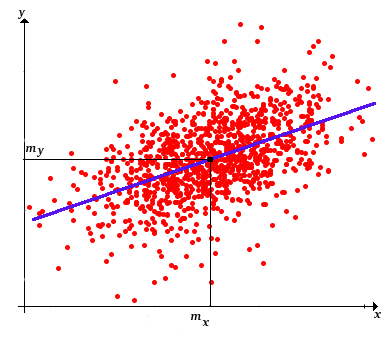
\includegraphics[scale=0.4]{reg_fallacy.png}
\end{center}
\caption{The regression fallacy}
\label{fig:fallacy}
\end{figure}

For example, we tend to experience ``football shaped'' scatterplots, such as that presented above. We see that all of the points are clustered around the mean (the blue regression line), but the observations which are extreme in both axes tend to be closer to the regression line.

It is important not to confuse a difference in the test scores with regression to the mean.










\chapter{Regression in causal inference}
\label{ch:causalreg}


Recall our discussion on causal inference. In this section, we introduced the Neyman-Rubin model of potential outcomes where we have two possible outcomes: the outcome if subject $i$ is assigned to treatment, $Y\_{i1}$, and the outcome if subject $i$ is assigned to control $Y\_{i0}$. For any given subject, we can only observe \textit{one} of these two outcomes, and we can write the response that we do observe as
$$Y_i = ( 1- T_i) Y_{i0} + T_i Y_{i1}$$

where $T_i$ is the treatment indicator (and is a \textit{random variable}) whereby $T_i = 1$ is subject $i$ is assigned to treatment and $T_i = 0$ if subject $i$ is assigned to control. We are interested in estimating the causal effect:
$$\frac{1}{N}\sum_{i=1}^N (Y_{i1} - Y_{i0})$$
which is an unobservable quantity that we typically estimate by the observed average outcome difference between the treatment and control groups:
$$\tau = \frac{1}{n_1} \sum_{i : T_i = 1} Y_i - \frac{1}{n_0} \sum_{i : T_i = 0} Y_i$$

It turns out that we can very naturally relate causal effect and linear regression. Suppose that we fit a linear model to the outcome using treatment assignment as the sole predictor:

$$Y_i = \beta_0 + \beta_1 T_i + \epsilon_i$$

Then $\beta$ can be thought of as the treatment effect on the outcome, and we can estimate it using OLS as described above. It can be shown that this estimate of the treatment effect is more or less equivalent to the simple estimator of the sample average treatment effect (SATE) of the form:

$$\tau = \frac{1}{n_1} \sum_{i : T_i = 1} Y_i - \frac{1}{n_0} \sum_{i : T_i = 0} Y_i$$

It is common to ``adjust for covariates'' by adding them into the regression equation

$$Y_i = \beta_0 + \beta_1 T_i + \beta_2 x_i +  \epsilon_i$$

however, the only reason we should ever even be \textit{tempted} to do this is if we believe that the covariate, $x$, is imbalanced between treatment and control in some way. This approach involving estimating the causal effect of the treatment by estimating $\beta_1$ using regression in which we adjust for covariates seems simple, and at first glance, very reasonable; in fact, this is the reason that this approach is so widely used (and misused!). There are however a huge number of critiques of this approach, primarily in the case of observational studies. One of the main issues is the assumption of \textit{linearity}. If this assumption is unjustified, then our OLS estimates will be significantly worse than the simple difference in means SATE estimates! Moreover, if we adjust for covariates in our linear model, it is often the case that we will introduce extra bias into our estimate of treatment effect! For example, Berk et al. (2010) claim that ``Random assignment does not justify any form of regression with covariates. If regression adjustments are introduced nevertheless, there is likely to be bias in any estimates of treatment effects and badly biased standard errors''. There are examples of adjustments for which this disparaging view of using regression to adjust for covariates is not justified (see, for an example, Lin (2010)), but these models should still be used with caution.

In general, the only reason we would want to use regression to estimate our causal effect is to adjust for covariates; if we did not feel that any of our covariates differed between the treatment and control group, then we might as well simply calculate the more general SATE estimator, $\tau$. If, however, we did feel concerned about covariate imbalance, then perhaps this adjusted regression is justified, however, there are a number of other approaches to consider: notable we might perform \textit{matching} which involves comparing subjects in the treatment to comparable subjects in the control group (where two subjects are comparable if they have similar covariate measurements).










\chapter{Generalized least squares}
\label{ch:gls}



\section{Weighted least squares}

Imagine that we want to fit a linear model, $y = X\beta + \epsilon$, where the error terms $\epsilon$ are assumed to be independent of $X$, but we do not believe the usual assumption that each of the error terms $\epsilon_i$ are iid with $E(\epsilon | X) = 0$ and $Cov(\epsilon | X) = \sigma^2 I$. In particular, what if we have reason to believe that the common variance assumption is violated. That is, instead of each error term having the same variance (homoskedasticity), we allow the error terms to each have different variances (heteroskedasticity):

$$Cov(\epsilon | X) = \Sigma = \left[ \begin{array}{cccc} \sigma_1^2 & 0 & \dots & 0\\
 0 & \sigma_{2}^2 & \dots & 0\\
 \vdots & \vdots & \ddots & \vdots\\
 0 & 0 & \dots & \sigma_{n}^2\end{array} \right]$$
 
 
Note that the standard OLS assumption of homoskedasticity corresponds to the case where $\sigma_1^2 = \sigma_2^2 = \dots = \sigma_n^2 = \sigma^2$. In the variance-covariance matrix above, we still assume \textit{independent} errors, but we no longer assume \textit{identically distributed} errors.

Heteroskedasticity is actually quite common, for example, suppose that we are interested in measuring household expenditure on meals as a function of household income. We might expect households of lower income to be more consistent in their food expenditure by always purchasing inexpensive food. Higher income households, on the other hand, will tend to be more variable in the amount they expend on their meals: on occasion, they will indulge in an extremely fancy and disturbingly expensive meal, while there will likely be other instances where they fall back on less expensive, yet more convenient meal options. Such an example of heteroskedasticity is demonstrated in the figure below, whereby we are observing household meal expenditure on a particular day versus income for 100 different households. We see that there is much less variability in the low-income households, whereas there is much more variability in the high-income households.


\begin{figure}[H]
\begin{center}
\includegraphics[scale=0.4]{heteroskedasticity.png}
\end{center}
\caption{heteroskedasticity}
\label{fig:heteroskedasticity}
\end{figure}


Given that for data which exhibits heteroskedasticity we are violating the iid assumption for the errors, can we still use the standard OLS procedure to estimate $\beta$? Technically, yes, we can use whatever estimator we want, however, whenever we violate model assumptions the estimates that we obtain are much less trustworthy. The question is, in what way are the estimates less trustworthy? Are they biased? Do they have incorrect variance? Are they even estimating the right thing? We will explore answers to these questions in the case of heteroskedaasticity below. \textcolor{red}{Come back to these questions}


\subsection*{Estimating $\beta$ in the presence of heteroskedasticity using weighted least squares}

To estimate $\beta$ when we do not have constant variance across observations, we can use a procedure called weighted least squares (WLS). The motivation behind WLS is that we have less confidence in observations which are extremely variable, and so we would like to reduce their influence on the least squares estimator by down-weighting such observations. In the presence of heteroskedasticity, the standard OLS estimator would be dominated by these noisy observations. Our goal is to reduce the impact of the imbalance of noise in our data. The WLS estimator can thus be written as

$$\hat{\beta}_{WLS} = \underset{\beta}{\text{argmin}} \sum_{i=1}^n \left(\frac{y_i - X_i^T \beta}{\sigma_i} \right)^2 = (y - X\beta)^T\Sigma^{-1}(y - X\beta)$$

where $\Sigma^{-1}$ is the inverse of the covariance matrix $\Sigma$, which, because $\Sigma$ is a diagonal matrix, the elements of the inverse are given by

$$\Sigma^{-1}_{ij} = \begin{cases} \frac{1}{\sigma_i^2} & \text{ if } i = j \\ 0 &\text{otherwise} \end{cases}$$

Let's define $W = \Sigma^{-1}$. Note that the difference between $\hat{\beta}_{WLS}$ and $\hat{\beta}_{OLS}$ is the fact that we are dividing (weighting) by $\sigma_i$ in the WLS estimator. It is not too hard to show that our WLS estimator $\hat{\beta}_{WLS}$ satisfies

$$(X^TWX)\hat{\beta}_{WLS} = X^TWy$$

(recall that our OLS estimator satisfied $(X^TX)\hat{\beta}_{OLS} = X^Ty$). So if $X^TWX$ is invertible, our estimator becomes

$$\hat{\beta}_{WLS} = (X^TWX)^{-1}X^TWy$$

This estimator is the maximum likelihood estimator of $\beta$ under hetersokedastic linear regression. Note that computation of this estimator requires that we know $W$, that is, we need to know the values of each of the $\sigma_i$s which is pretty much never the case. In the next section, we will generalize this idea further, and discuss how to estimate $\beta$ even when we don't know the true values of the $\sigma_i$.






\section{Generalized least squares}

Next, we ask the question of what happens if we violate even more assumptions? For example, in the WLS situation above, we had violated the assumption that the error terms were identically distributed (by allowing for heteroskedasticity), but what happens if we also violate the assumption of independence? We can write this more general situation as



$$Cov(\epsilon | X) = G = \left[ \begin{array}{cccc} \sigma_{11} &  \sigma_{12} & \dots & \sigma_{1n}\\
 \sigma_{21} & \sigma_{22} & \dots & \sigma_{2n}\\
 \vdots & \vdots & \ddots & \vdots\\
 \sigma_{n1} & \sigma_{n2} & \dots & \sigma_{nn}\end{array} \right]$$

where $\sigma_{ii} = \sigma_i^2$ is the variance of observation $i$, and $\sigma_{ij}$ is the covariance between observation $i$ and $j$. The WLS case discussed above corresponds to the special case where each of the $\sigma_{ij}$ with $i \neq j$ are 0. To conduct least squares in this more general case, instead of weighting only by the diagonal elements $\sigma_{ii}$, we weight by the entire covariance matrix, $G$:

$$\hat{\beta}_{GLS} = \underset{\beta}{\text{argmin}} (y - X\beta)^T G^{-1}(y - X\beta)$$

Note that if $G$ is positive definite, then we can turn the above formulation into a standard OLS-type problem. Let's assume momentarily that $G$ is known (an unfortunately unrealistic assumption in real life), then since $G$ is positive definite, the SVD of $G$ tells us that there exists an orthogonal matrix $R$ and a diagonal matrix $D$ (whose entries are positive) such that $G = RDR^T$. We can thus calculate $G^{-1}$, $G^{\frac12}$ and $G^{-\frac12}$ as follows:
$$G^{-1} = RD^{-1}R^T, ~~~~~~G^{\frac12} = RD^{\frac12}R^T, ~~~~~~ G^{-\frac12} = RD^{-\frac12}R^T$$

This implies that we can write $G^{-1} = G^{-\frac12}G^{-\frac12}$ (note that it is not true of all matrices, $M$ that such a decomposition into ``square-roots'', $M^{\frac12}$, exists, but since $G$ was positive definite, we were able to use properties of orthogonal and diagonal matrices to explicitly show that such decompositions existed), and so

\begin{align*}
(y - X\beta)^T G^{-1}(y - X\beta) &= (y - X\beta)^T G^{-\frac12} G^{-\frac12}(y - X\beta)	
& = \left(G^{-\frac12} y - G^{-\frac12}X \beta\right)^T\left(G^{-\frac12}y - G^{-\frac12}X\beta\right)
\end{align*}

Thus, we can write

$$\hat{\beta}_{GLS} = \underset{\beta}{\text{argmin}} (\tilde{y} - \tilde{X}\beta)^T (\tilde{y} - \tilde{X}\beta)$$

where $\tilde{y} = G^{-\frac12}y$ and $\tilde{X} = G^{-\frac12} X$. Notice that this is just a standard OLS problem on $\tilde{y}$ and $\tilde{X}$! Thus, if we knew $G$ and were thus able to calculate $\tilde{X}$ and $\tilde{y}$, then we could estimate $\beta$ by the usual OLS estimator: $$(\tilde{X}^T\tilde{X})^{-1}\tilde{X}^T\tilde{y}$$

In reality however, the true covariance matrix, $G$, is rarely known.



\subsection*{Estimating $\hat{\beta}_{WLS}$ when the covariance matrix, $G$, is unknown}

In general, we can solve 






\chapter{The challenger O-ring failure}
\label{ch:gls}





In January of 1986, the NASA space shuttle orbiter \textit{Challenger} mission ended in disaster when the shuttle broke apart 73 seconds into its flight, killing all seven crew members on board. This incident is considered one of the worst space disasters of all time. The disintegration was caused by the failure of an O-ring seal which allowed pressurized burning gas to escape from within the solid rocket motor resulting in aerodynamic forces breaking up the shuttle.

These O-ring seals had been tested and shown to keep its their seal in temperatures as low as 40 degrees Fahrenheit, but on the morning of liftoff, the temperature was a mere 18 degrees Fahrenheit, a temperature described by Bob Ebeling from Thiokol as ``no man's land'' in terms of the range of temperatures considered to be safe for liftoff. The plot below shows the number of O-ring failures at each of 23 temperatures tested.





\begin{figure}[H]
\begin{center}
\includegraphics[scale=0.8]{oring.png}
\end{center}
\caption{O-ring data}
\label{fig:oring}
\end{figure}



How could the analysts have predicted whether or not the O-ring would fail at 18 degrees Fahrenheit? Should we simply use our test observations to fit a linear model of the form: $\text{failure} = \beta\_0 + \beta\_1 \times \text{temperature} + \epsilon$? We could try, but it is unnecessary. The recommended approach, contrary to what you might be expecting, is to just \textit{look at the data}! You don't need to fit fancy models or do fancy hypothesis tests to see that for all tests performed below 65 degrees, at least one of the O-rings failed. Surely if the analysts had actually \textit{looked} at the data, they would not have recommended that the liftoff take place.


<!--
One approach might have been to use OLS to fit a linear model of the form

$$\text{failure} = \beta_0 + \beta_1 \times \text{temperature} + \epsilon$$

where we could estimate $\beta_0$ and $\beta_1$ using the 23 observations we already had. This is 
-->








\chapter{Alternatives to least squares (M-estimation)}
\label{ch:mest}





Above we have focused primarily on estimating $\beta$ in the model $y = X\beta  + \epsilon$ by minimizing the squared loss function (or weighted versions of it):

$$\hat{\beta}_{OLS} = \underset{\beta}{\text{argmin}} \sum_{i=1}^n (y_i - X_i^T \beta)^2$$

but what's stopping us from using other types of loss functions? The answer is: absolutely nothing! This prompts us to define a general M-estimator (of which least squares is an example): an M-estimate of $\beta$ is any estimator that can be written in the following form

$$\hat{\beta} = \underset{\beta}{\text{argmin}} \sum_{i=1}^n \rho(y_i - X_i^T \beta)$$

where $\rho$ is any suitable function. For example

\begin{itemize}
\item $\rho(x) = x^2$ gives us the ordinary least squares estimator.
\item $\rho(x) = \vert x \vert$ gives us the least absolute deviation (LAD) estimator.
\end{itemize}


If in general, we consider the OLS estimate as a generalization of the mean ($\underset{a}{\text{argmin}} \sum_{i=1}^n (x_i - a)^2 = \bar{x}$), then the LAD estimate can be thought of as a generalization of the median ($\underset{a}{\text{argmin}} \sum_{i=1}^n |x_i - a| = \text{median}(x)$). The LAD is in general much more robust to outliers than the OLS estimator, but it does not confer a closed-form solution (recall that the closed-form solution for the OLS estimator is $\hat{\beta}_{OLS} = (X^TX)^{-1}X^Ty$). So how can we use LAD to estimate $\beta$?

We can use the fact that $\frac{\vert X \vert^2}{\vert X \vert} = \vert X \vert$ to iteratively compute the LAD estimate using weighted least squares. The procedure is as follows: 


\begin{enumerate}
\item Choose an initial estimate (typically we use the standard OLS estimator as our starting point) $$\hat{\beta}^{(0)} = \hat{\beta}_{OLS}$$.
\item Given a current estimate, $\hat{\beta}^{(t)}$, calculate a new LAD estimate by solving
\begin{align*}
\hat{\beta}^{(t + 1)} & = \underset{\beta}{\text{argmin}} \sum_{i=1}^n \frac{\Big\vert y_i - X_i^T \beta \Big\vert^2}{\Big\vert y_i - X_i^T \beta^{(t)} \Big\vert}\\
& =  \underset{\beta}{\text{argmin}} \sum_{i=1}^n w_i(t) \Big\vert y_i - X_i^T \beta \Big\vert^2
\end{align*}
where $w_i(t) = \frac{1}{\Big\vert y_i - X_i^T \hat{\beta}^{(t)} \Big\vert}.$
\item Continue until convergence has been achieved.
\end{enumerate}

Note that this is equivalent to iteratively solving a WLS problem.



Since the LAD estimator is more robust than the OLS estimator, shouldn't we just always use the LAD estimator? Can you think of an example of why not? Essentially this question boils down to whether or not the median is ``better'' than the mean as an estimator of a ``typical value''. In reality, which provides a better estimator depends on what you mean by typical. As an example, consider reporting housing prices in a particular area. If the area consists of mostly moderately sized houses but there are a few extremely large houses, then these large houses will have a large influence on the mean house price (it will inflate it significantly and give a misleading sense of how nice the houses in the area are), but they will have little effect on the median house price. In this situation, since we are interested in the house of a ``typical'' house in the area, it makes sense to look at the median house price rather than the mean. On the other hand, if the outliers are informative in terms of the questions being asked, then you don't want to ignore them by using a robust estimator or deleting the observations! 









\part{Prediction}



\chapter{Prediction}
\label{ch:pred}




Much of science, social science and engineering is about finding relationships between predictor variables, typically stored in a matrix $X$, and a response variable, typically stored in a vector, $y$. For example, we might be interested in using socio-economic variables of various communities to predict the corresponding crime rate in those communities, or we could use features extracted from images to predict the response of the brain to viewings of those images. If the response variables are observable or measurable (for example crime rate, brain response, diseased/healthy), then the process of connecting predictor variables to response variables is called \textit{supervised learning}. This is in contrast to \textit{unsupervised learning}, described in previous sections, where our response variable was not observed (recall our discussion on clustering: the clusters were our response variable, but we had not a priori defined the cluster groups in our data). Both supervised and unsupervised learning approaches fall into the monolithic category of \textit{machine learning}, which we will only touch upon here.




Supervised learning is an umbrella term for two primary classes of problems: \textit{regression} for continuous responses (such as brain activity or crime rate), and \textit{classification} for discrete categorical responses (such as an indicator specifying whether an individual is healthy or diseased). A plethora of resources exist for classification tools such as (in order of increasing complexity) discriminant analysis techniques, classification trees (extending to random forests), support vector machines and neural networks, but we will only touch upon them here.


Even for basic science research, good prediction should be one of the primary goals when generating data models. If a model is unable to adequately predict reality, then it is hard to believe that the model is capable of capturing the underlying mechanisms that dictate the relationship between predictor and response. However, this is not always the case, we will see below an extremely simple example of an incorrectly specified model that generates more accurate predictions than a correctly specified model.


\section{Regularization: a motivational example}

It is interesting to note that it is entirely possible that an ``incorrect'' model can provide better predictions than a ``correct'' model. For a simple example, suppose that we have $n$ observations, $X_1, ..., X_n$ which are independently and identically distributed $N(\theta, \sigma^2)$ random variables, where we know $\sigma^2$ (say, $\sigma^2 = 1$, for example), but we don't know $\theta$. Our goal is to predict the next observation in the sequence, $X_{n + 1}$, which follows the same distribution as each of the previous $n$ variables and is independent of them. First of all, what kind of model might we come up with to predict $X_{n + 1}$? If we knew the distribution of these random variables, then we could simply predict that $X_{n + 1}$ will be the most likely observation to be drawn from that distribution (for example, the mean), but all we know is that the observations are normally distributed: the mean, $\theta$, is unknown, so we must estimate it! 

Let's compare two possible models. In the first model, our background knowledge gave us confidence to assume that $\theta \approx 0$ (even though $\theta = 0$ is probably incorrect), that is, we are assuming that each observation is drawn from a Gaussian distribution with $0$ mean and some known variance $\sigma^2$. In the second model, we have no idea about what the true mean might be, other than knowing that it is nonzero, so we assume only that $\theta \neq 0$. In this second model, each observation is drawn from a Gaussian distribution with some unknown (but presumably nonzero) mean, $\theta$. In Model 1, the mean of the distribution of $X_{n + 1}$ is assumed to be 0, so it makes sense that our prediction for $X_{n + 1}$ would be 0. In Model 2, however, we don't know the true mean, so we must estimate it! Given that we have $n$ observations drawn from this $N(\theta, \sigma^2)$ distribution, what estimator can you think of for the population mean, $\theta$? Hopefully, the first thing that came to your mind was the sample mean of the existing observations: $\hat{\theta} = \overline{X}_n = \frac{1}{n} \sum_{i = 1}^n X_i$. It is not hard to show that this estimator is the \textit{maximum likelihood} estimator. So to summarize:


\begin{itemize}
\item \textbf{Model 1}: assume that $X_i \sim N(0, 1)$ so we chose $\hat{X}_{n + 1} = 0$.
\item \textbf{Model 2}: assume that $X_i \sim N(\theta, 1)$ where $\theta \neq 0$, so we chose $\hat{X}_{n + 1} = \overline{X}_n$.
\end{itemize}


To assess which of these models yield better predictions for $X_{n + 1}$ we want to compare the \textit{prediction error} for the estimators $\hat{X}_{n + 1} = 0$ and $\hat{X}_{n + 1} = \bar{X}$. The prediction error describes how close our predictions, $\hat{X}_{n + 1}$, are to the real value $X_{n + 1}$. We can use the Mean Squared Error (MSE) as a measure of the prediction error:

$$\text{MSE}(\hat{X}_{n + 1}) = E\left( \hat{X}_{n + 1} - X_{n + 1}\right)^2$$


Recall that we still don't know the value of $\theta$, all we know is that $X_{n + 1} \sim N(\theta, \sigma^2)$, so for Model 1, where we used the estimate $\hat{X}_{n + 1} = 0$, we have

$$\text{MSE}_{\text{Model 1}}(\hat{X}_{n + 1}) = E(X_{n + 1}^2) = Var(X_{n + 1}) + E(X_{n + 1})^2 = \sigma^2 + \theta^2$$

On the other hand, for Model 2, where we used the estimate $\hat{X}_{n + 1} = \overline{X}_n$, we have

$$\text{MSE}_{\text{Model 2}}(\hat{X}_{n + 1}) =  E(\overline{X}_n - X_{n + 1})^2 = E(\overline{X}_{n}^2) - 2E(X_{n + 1}\overline{X}_{n}) + E(X_{n + 1}^2)$$

Note that $\overline{X}_n \sim N\left(\theta, \frac{\sigma^2}{n}\right)$ (if you aren't familiar with this result, you should show it yourself!), and $X_{n + 1}$ is independent of $\overline{X}_n$, so the above expression simplifies to

\begin{align*}
\text{MSE}_{\text{Model 2}}(\hat{X}_{n + 1}) &=  E\left(\overline{X}_{n}^2\right) - 2E(X_{n + 1})E(\overline{X}_{n}) + E(X_{n + 1}^2)\\
& = \left(\frac{\sigma^2}{n} + \theta^2\right) - 2 \theta^2  + (\sigma^2 + \theta^2)\\
& = \frac{\sigma^2}{n} + \sigma^2
\end{align*}


So which model has the smallest prediction error? If the true value of $\theta$ is not too far from $0$ (more specifically, if $|\theta| < \frac{\sigma}{\sqrt{n}}$), then Model 1 has the smaller prediction error, even though the true value of $\theta$ might not be exactly $0$! To rephrase from another perspective: even though Model 2 provides an \textit{unbiased estimator} (the sample mean is an unbiased estimator for $\theta$), it is less accurate than the biased estimator of $\hat{X}_{n + 1} = 0$ from Model 1 (which makes the fairly strong - and likely incorrect - assumption that $\theta = 0$) \textit{more accurately} predicts the true value of $X_{n + 1}$ even though the true value of $\theta$ might not be 0 at all!

Perhaps at this point you're thinking ``how can a biased estimator be better than a biased estimator?''. If so, perhaps it's time to have a re-read of our discussion of the bias-variance tradeoff! Estimators with high bias tend to also have low variance and vice versa. Thus, sometimes we can decrease the overall MSE by adding a little bit of bias if this helps to significantly reduce the variance. This concept is known as \textit{regularization} and is highly utilized in high-dimensional techniques.


\section{Set-up: prediction problems}


To frame prediction problems in a more technical way: given training data $x_i$, $i = 1, ..., n$, where each $x_i$ is a vector of length $p$ containing a value for each of our $p$ variables of interest (for example for the $i$th person in our dataset we might record the following predictor variables $x_i = (gender_i, age_i, weight_i, glucose_i, insulin_i)$) we would like to predict a response variable $y_i$ (such as $y_i = diabetes_i$). The general approach find a prediction rule, $f(x_i)$ which maps the predictor vector to a response so that ideally we should have $f(x_i) \approx y_i$. Then, given the predictor values, $x$, of a new observation, we can predict the unobserved response variable, $y$, using ${\bf \hat{y}} = f({\bf x})$. In general, the response $y_i$ is a single value, but there are many cases where we want to predict multiple responses (so that $y_i$ is a vector), in which case we call such a problem a \textit{multi-response prediction problem}.

What are we assuming by defining some prediction rule, $f$? We're assuming that the situations or observations presented in the training data are similar (in terms of the relationship between predictor and response) to new situations where for which want to predict the outcome. If this is true, then the prediction rules that we defined using our training data are applicable to new predictor variables, and we will obtain reasonable predictions. It might be surprising that in a vast number of situations, this is not the case. For example, it might be the case that the new predictor variables were measured using a different instrument to the old predictor variables, resulting in a slightly different relationship to the response variable.





\section{Binary prediction methods: classification}

In the section above, we discussed the ultimate goal in binary prediction which is to come up with some prediction rule, $f$, such that ${\bf \hat{y}} = f({\bf x})$ is a good approximation to the true classification vector, ${\bf y}$, where ${\bf y}$ is a binary vector consisting of $0$'s and $1$'s, where, for example suppose that we have 9 observations whose true class is given by ${\bf y} = (0, 1, 1, 1, 0, 0, 1, 0, 1)$. This implies that the first observation is in class 0 (e.g. do not have diabetes), while the second, third and fourth observations are in class 1 (e.g. do have diabetes). We want to be able to use the information contained in the predictor variables ${\bf x}_i = (x_{i1}, ..., x_{ip})$, for $i = 1, ..., 9$, to come up with a rule to predict ${\bf y}$. For example, we may end up with ${\bf \hat{y}} = f({\bf x}) = (0, 0, 1, 1, 0, 1, 1, 0, 1)$, which is similar to the true classification vector, ${\bf y}$, but observations two and six are misclassified.









\chapter{Binary prediction methods (classification)}
\label{ch:class}



Suppose that we have $n$ observations each of which fall into one of two categories, which for notational simplicity, we will call 0 and 1. We define the response or class vector to be the vector ${\bf y} = (y_1, ..., y_n)$, where 
$$y_i = \begin{cases} 0 & \text{ if observation $i$ belongs to class $0$}\\ 1 & \text{ if observation $i$ belongs to class $1$} \end{cases}$$

Along with each observation, $i$, we have a vector of $p$ predictor variables, ${\bf x}_i =  (x_{i1}, ..., x_{ip})$, that might be considered relevant for predicting which of the two classes the observation belongs. The problem of interest is how to define a prediction rule, $f$, which is a function of the the predictors, $x = ({\bf x}_1, ..., {\bf x}_p)$, such that $f({\bf x}) \approx {\bf y}$. 

This section focuses on identifying the most common functions, $f$, that we might like to consider.




\section{Linear discriminant analysis (LDA)}

Linear discriminant analysis (LDA) aims to find a linear (or planar) boundary between the two classes in the predictor space, and any new observations are classified according to which region of space their predictors fall into. This is easy to visualize using a simple two-dimensional example, whereby we have two classes (red and blue) and two predictor variables. The figure below shows one predictor variable plotted against the other, and the color corresponds to the class of each observation. We can see that there is a fairly clear boundary between the two classes based on this two-dimensional predictor space.

\begin{figure}[H]
\begin{center}
\includegraphics[scale=0.8]{lda.png}
\end{center}
\caption{LDA}
\label{fig:lda}
\end{figure}

However, we note that this boundary line is not perfect, there are some blue points that fall below it and some red points that fall above it, but we note that using a linear boundary it is not possible to perfectly classify every point.

How do we define this LDA boundary? \textcolor{red}{Give the details!}


\section{Quadratic discriminant analysis (QDA)}

Much like LDA but uses a quadratic boundary instead of a linear boundary \textcolor{red}{Give the details!}


\section{Logistic regression}

Logistic regression can be thought of as a generalized linear model (we will discuss glms further in a later section). Note that in contrast to generalized least squares, which was a generalized method of estimating the coefficients in a standard linear model, generalized linear models generalize the form of the model itself. For instance, suppose that we had a binary outcome, where each individual's response was either a 0 (e.g. non-diabetic) or a 1 (diabetic), and we had a number of predictor variables (age, weight, height, gender, etc). A naive approach to predicting diabetes might be to fit a linear model of the form


$$diabetes = \beta_0 + \beta_1 age + \beta_2 weight + \beta_3 height + \beta_4 gender + \epsilon$$

and then use OLS, GLS, LAD, etc to estimate the coefficients. What's the problem with this approach? First of all, there's no guarantee that once we've fitted the model (estimated the coefficients), that the predicted response, 
$$\widehat{diabetes} = \hat{\beta}_0 + \hat{\beta}_1 age + \hat{\beta}_2 weight + \hat{\beta}_3 height + \hat{\beta}_4 gender$$
will even be in $\{0, 1\}$, in fact, this is extremely unlikely!

Supposing that we were really attached to the linear model idea, what alternative routes could we take? Perhaps instead of modelling the response itself as a linear combination of our predictors, we could model the probability of the response being $1$ as a function of a linear combination of our predictors (where the function is defined so that we obtain a probability between 0 and 1). More specifically, we could define the \textit{logistic regression model} given by

$$P(y_i = 1 | x_i) = \frac{e^{\beta_0 + \beta_1x_{i1} + ... + \beta_px_{ip}} }{1 + e^{\beta_0 + \beta_1x_{i1} + ... + \beta_px_{ip}}} = \frac{e^{x_i^T \boldsymbol{\beta}} }{1 + e^{x_i^T \boldsymbol{\beta}}}$$

where, as with standard linear regression, we want to estimate the $\beta$ vector. Recall that in standard linear regression, we have $E(y_i | x_i) = x_i^T\beta$, and $Var(y_i | x_i) = Var(\epsilon_i) = \sigma^2$, so that if we assumed normality of the $\epsilon_i$'s, we had 
$$y_i | x_i \sim N(x_i^T\beta, \sigma^2)$$

the corresponding distributional result assumed by logistic regression is
$$y_i | x_i \sim Bernoulli\left(\frac{e^{x_i^T \boldsymbol{\beta}} }{1 + e^{x_i^T \boldsymbol{\beta}}}\right)$$


Next, we can define the \textit{log-odds ratio} by
$$\log \left(\frac{P(y_i = 1 | x_i)}{P(y_i = 0 | x_i)} \right) = \log  \left(\frac{P(y_i = 1 | x_i)}{1 - P(y_i = 1 | x_i)} \right) = \log \left( e^{x_i^T \beta} \right) = x_i^T \beta$$

In an attempt to foreshadow later results, we will eventually refer to the log-odds as the \textit{link function} for logistic regression. The link function describes how the response is ``linked'' to the linear combination of the predictors (for standard linear regression, the link function is simply $g(x) = x$).



How do we convert the logistic regression model into class predictions? Given a new sample $x_i^*$, we can plug it into the fitted logistic model

$$P(y_i^* = 1 | x_i^*) = \frac{e^{x_i^{*T} \boldsymbol{\hat{\beta}}} }{1 + e^{x_i^{*T} \boldsymbol{\hat{\beta}}}}$$

and we might define our prediction rule to be

$$\hat{y}_i^* = \begin{cases} 1 & \text{ if $P(y_i^* = 1 | x_i^*) > 0.5$}\\ 0 & \text{ otherwise}\end{cases}$$

so that if the estimated probability of being in class $1$ is greater than $0.5$, then we predict that the observation is in class $1$. Although we need not use the cutoff of $0.5$, it is not uncommon to use the cutoff that minimizes the misclassification rate (see the next section).


\subsection*{Fitting the logistic regression model}


In the previous section, we have discussed how to use logistic regression to obtain a class prediction for an observation. However, to do this, we need to know how to estimate $\beta$. This is not as straightforward as using least squares for the standard linear regression model for which we wanted to find the value of $\beta$ that minimized the squared loss $\sum_{i=1}^n (y_i - x_i\beta)^2$, for which we could find a closed form solution $\hat{\beta}_{OLS} = (X^TX)^{-1} X^T y$. 

In the case of the logistic regression model, the least squares estimate for $\beta$ would be defined by 
$$\hat{\beta}_{LS} = \underset{\beta}{\text{argmin}} \sum_{i=1}^n \left(y_i -  \frac{e^{x_i^T \beta}}{1 + e^{x_i^T \beta}}\right)^2$$ 

However, this estimate is rarely used for multiple reasons. The first is that it cannot be computed explicitly (there is no closed-form solution), and must be estimated using numerical methods (we will discuss these further below). Moreover, least squares in the context of logistic regression is no longer optimal. For the standard linear model case, it was possible to show that the least squares estimate of $\beta$ was the same as the \textit{maximum likelihood estimate} (MLE) of $\beta$, and thus was the best estimator (in the sense that it had the lowest MSE). In the case of logistic regression, however, the least squares estimator yields an estimator distinct from the MLE, implying that the least suqares estimator is no longer the ideal estimator. The following steps walk us through deriving the MLE for logistic regression, where the MLE estimate for $\beta$ is the value of $\beta$ that maximizes the likelihood function (or, equivalently, the log-likelihood function).

First, assuming that the $y_i | x_i$'s are independent (this assumption is extremely important for inference, but somewhat less important for prediction if we have a proper test set with which to evaluate the prediction accuracy), the likelihood can be split up into

$$L(y_1, y_2, ..., y_n | x) = L(y_1 | x_1) \cdot L(y_2 | x_2)  \cdot \dots \cdot L(y_n | x_n) $$

Thus, if we define $\pi_i = P(y_i = 1 | x_i) = \frac{e^{x_i^T \boldsymbol{\beta}} }{1 + e^{x_i^T \boldsymbol{\beta}}} $ to be the true probability that observation $i$ is in class 1, then 

$$L(y_1, y_2, ..., y_n | x) = \prod_{i=1}^n \pi_i^{y_i} ( 1 - \pi_i)^{1 - y_i} $$


in which case, the log-likelihood can be written as

\begin{align*}
\ell(y_1, ..., y_n | x) & = \log L(y_1, ..., y_n | x)\\
& = \sum_{i=1}^n \left( y_i \log \pi_i + ( 1- y_i) \log ( 1 - \pi_i)\right)\\
& = \sum_{i=1}^n \left( y_i \log \frac{\pi_i }{1- \pi_i} + \log (1 - \pi_i) \right)\\
& = \sum_{i=1}^n \left( y_i x_i^T \beta - \log \left( 1 + e^{x_i^T \beta} \right) \right) 
\end{align*}


where the last equality follows from the fact that $1 - \pi_i = \frac{1}{1 + e^{x_i^T \beta}}$.



To calculate the maximum likelihood estimator of $\beta$, we would need to find the value of $\beta$ that maximizes the above log-likelihood expression. Further, supposing that this value is denoted by $\hat{\beta}_{MLE}$, we could predict the class for a new observation with predictor vector, $x$, by

$$\hat{y} = \begin{cases} 0 & \text{ if } \hat{\pi}^{MLE} = \frac{e^{x^T \boldsymbol{\hat{\beta}}_{MLE}} }{1 + e^{x^T \boldsymbol{\hat{\beta}}_{MLE}}} < 0.5 \\ 
 1 & \text{ if } \hat{\pi}^{MLE} = \frac{e^{x^T \boldsymbol{\hat{\beta}}_{MLE}} }{1 + e^{x^T \boldsymbol{\hat{\beta}}_{MLE}}} \geq 0.5\end{cases}$$


However, unfortunately, there is no closed-form solution for the maximum of the log-likelihood function given above, implying that we cannot simply find n explicit formula for the MLE estimator. However, fortunately, we are able to estimate the MLE using numerical methods such as Newton-Rhapson or iteratively weighted least squares (IWLS). The technical details of these iterative approaches are provided in the appendix for the interested reader. One point to note is that, as with any iterative procedure, it is important to check the convergence criteria: the NR or IWLS procedures will converge to the true minimum (or maximum), but we need to ensure that we have run through a sufficient number of iterations to have achieved convergence. When implemented in the software, such methods typically have a default number of iterations, however, for some problems, this default may not be enough to ensure convergence, and as such, it is important to check convergence criteria.



\section{A comparison of least squares and maximum likelihood for binary responses}

To summarize the discussion above, we discussed how to estimate $\beta$ for the logistic regression model for binary responses. The logistic regression model assumed that

$$y_i| x_i \sim Bernoulli\left(\frac{e^{x_i^T \boldsymbol{\beta}} }{1 + e^{x_i^T \boldsymbol{\beta}}}\right)$$

and we discussed the fact that the LS estimator of $\beta$ based on this model,

$$\hat{\beta}_{LS} = \underset{\beta}{\text{argmin}} \sum_{i=1}^n \left(y_i -  \frac{e^{x_i^T \beta}}{1 + e^{x_i^T \beta}}\right)^2$$

was less optimal than the MLE estimator defined by

$$\hat{\beta}_{MLE} = \underset{\beta}{\text{argmax}}\sum_{i=1}^n \left( y_i x_i^T \beta - \log \left( 1 + e^{x_i^T \beta} \right) \right) $$



However, in this section we will discuss how the  \textit{OLS estimator for the standard linear regression model} compares with the \textit{MLE estimator for the logistic regression model}? That is, we are comparing the standard linear model OLS formulation

$$\hat{\beta}_{OLS} = \underset{\beta}{\text{argmin}} \sum_{i=1}^n \left(y_i -  \frac{e^{x_i^T \beta}}{1 + e^{x_i^T \beta}}\right)^2 ~~~~~ \text{where} ~~~~ y_i | x_i \sim N(x_i^T\beta, \sigma^2)$$

with the losgistic regression MLE formulation

$$\hat{\beta}_{MLE} = \underset{\beta}{\text{argmax}}\sum_{i=1}^n \left( y_i x_i^T \beta - \log \left( 1 + e^{x_i^T \beta} \right) \right) ~~~~~ \text{where} ~~~~ y_i | x_i \sim Bernoulli\left(\frac{e^{x_i^T \boldsymbol{\beta}} }{1 + e^{x_i^T \boldsymbol{\beta}}}\right)$$


The figure below displays contour maps for the estimates of $\beta_0$ and $\beta_1$ for the O-ring data when we use the log-likelihood estimate for logistic regression and when we use the least squares estimate for the standard linear regresssion. 



\begin{figure}[H]
\begin{center}
\includegraphics[scale=0.5]{ls_vs_mle.png}
\end{center}
\caption{Contour maps for LS and MLE for binary responses}
\label{fig:ls_vs_mle}
\end{figure}

These graphs display the contour lines of the surface for the two loss-functions. The minimum point is shown on each plot: the ``o'' corresponds to the OLS estimator (corresponding to the minimum of the right plot) and the ``x'' corresponds to the MLE estimator (corresponding to the minimum of the left plot). One thing to notice is that the logistic regression surface does not exhibit symmetry whereas the linear regression surface does. What we are seeing however, is that the estimate obtained from the MLE (log-likelihood) for the logistic regression model is fairly similar to the estimate obtained from least squares on the standard regression model. \textcolor{red}{will need to come back to this...}





\section{MLE in high-dimensions}

In the setting where $X$ is high-dimensional (when we have many variables), if we use the MLE to fit models, we are typically faced with the issue of overfitting and instability. More specifically, the decision rules generated in high dimensions will be stable, but the estimates of $\beta$ are not. As a result, the predictions drawn from such models will be inaccurate on new data when the model was fit using $\hat{\beta}_{MLE}$. As such, when fitting a model using high dimensional data, we should begin by performing dimension reduction. The are two main approaches to dimension reduction that we will consider here: feature (variable) selection and penalization/regularization.

\subsection*{Feature selection}

One way to reduce the dimension of our data is to identify the most informative variables which we will use to build a model. The problem of feature selection hosts a wide array of literature, and a plethora of methods exist. One of the most intuitive, and simple, approaches to feature selection is to simply select the features whose values are most correlated with the response of interest. Alternatively, we could use some prespecified criterion such as the AIC or BIC step-wise procedures which describe how much a model is improved by including or excluding each individual variable (however, the AIC and BIC approaches are not recommended). Another approach is to perform PCA, whereby we could either use the first few principal components (or those who explain the majority of the variability in the data) as our new variables, or if we wished to retain the original interpretability of our features, we could identify the original variables that were the most correlated with the first few principal components.





\subsection*{Regularization}

We will discuss regularization in detail later, but the overall idea is that we can put constraints on the $L^1$-norm of the $\beta$ estimator which has the effect of shrinking many of the coefficients contained in the $\hat{\beta}$-vector to zero. The variables of interest would be those whose coefficients were non-zero. This estimator of the shrunken coefficients is usually referred to as the \textit{lasso} estimator.



\section{Random forest (RF)}




\section{Support vector machines (SVM)}




\section{Appendix: Estimating the MLE for logistic regression using Newton-Rhapson}


The general outline of the quadratic iteratively weighted least squares (IWLS) and linear Newton-Rhapson (NR) iterative approaches both begin by define the initial estimate of $\beta$ to be $\hat{\beta}^{(0)} := \hat{\beta}_{OLS}$. The IWLS approach involves performing iterative quadratic approximations whereby we identify the maximum of the quadratic function at each iteration and use this maximum as the location of the quadratic approximation for the next iteration. In this case, the least squares weight is obtained from the previous iteration. The alternative linear (Newton-Rhapson) approach instead involves solving $\ell^\prime(\beta) = 0$ using iterative linear approximations for which we identify the root in each iteration and use this root as the location for our next linear approximation.

It turns out, however, that the quadratic and linear approximations described above are equivalent, since identifying the maximum of the quadratic approximation to $\ell(\beta)$ corresponds to identifying the root of the linear approximation to $\ell^\prime(\beta)$. Thus, in the details below, we focus on the technical details of the Newton-Rhapson approach only.


\subsection**{The $1$-dimensional case: $\beta \in \mathbb{R}$}

Let's define the \textit{score function} by

$$U(\beta) = \frac{d \ell(\beta)}{d \beta} = \sum_{i=1}^n \left( y_i x_i - \frac{x_i e^{x_i \beta}}{1 + e^{x_i \beta}}\right)$$

Finding the MLE of $\beta$ corresponds to seeking a solution to $U(\beta) = 0$, and since there is no closed-form solution to this problem, the Newton-Rhapson method estimates a solution to $U(\beta) = 0$ using iterated linear approximations, whereby at each iteration, we aim to improve upon the estimate of the previous iteration. 

To begin, we typically set the initial estimator of the logistic regression MLE to be the least-squares estimator of a standard linear regression model:

$$\beta^{(0)} := \hat{\beta}_{LS}$$

Next, the $m$th estimate of $\beta$ is found by solving

$$U^{(m)}(\beta) = 0$$

where $U^{(m)}(\cdot)$ is the linear approximation of $U(\cdot)$ at the estimate obtained from the previous iteration, $\beta = \beta^{(m-1)}$. More specifically, we can estimate the score function at the $m$th iteration, $U^{(m)}(\beta)$, by 

$$U^{(m)}(\beta) \approx U\left( \beta^{(m-1)}\right) + \frac{dU}{d\beta} \Big\vert_{\beta = \beta^{(m-1)}} \left( \beta - \beta^{(m-1)} \right)$$

which is reminiscent of a first-order Taylor expansion of $U(\cdot)$ about $\beta^{(m-1)}$. 

Next, setting $U^{(m)}(\beta)$ to zero, and solving for $\beta$ to get $\beta^{(m)}$ the new estimate, we obtain

$$\beta^{(m)} = \beta^{(m-1)} + \left[ - \frac{dU}{d\beta} \Big\vert_{\beta = \beta^{(m-1)}} \right]^{-1} U\left(\beta^{(m-1)}\right)$$


Note that

$$\frac{dU}{d\beta} = \frac{d^2 \ell(\beta)}{d\beta^2}$$

and the \textit{observed Fisher information} matrix is defined to be

$$I = - \frac{d^2 \ell}{d\beta^2}$$

\subsection**{The $p$-dimensional case: $\beta \in \mathbb{R}$}

We now consider the $p$-dimensional case (where the number of variables, $p \geq 1$). In this case, we are trying to 

In this case, we are trying to estimate a $p$-dimensional vector, $\beta \in \mathbb{R}^p$, rather than a scalar. Fortunately, an equivalent iterative formula exists for the multidimensional case, where the value of $\beta$ at the $m$th iteration, $\beta^{(m)}$, can be found by calculating

$$\beta^{(m)} = \beta^{(m-1)} + \left[ - \frac{\partial^2 \ell}{\partial \beta_i \partial \beta_j} \Big\vert_{\beta = \beta^{(m-1)}} \right]^{-1} U\left(\beta^{(m-1)} \right)$$

where $U(\beta) = \left( \frac{\partial \ell}{\partial \beta_1}, ..., \frac{\partial \ell}{\partial \beta_p} \right)$. In this case, the observed Fisher information matrix is defined to be

$$I = - \frac{\partial^2 \ell}{\partial \beta_i \partial \beta_j}$$

Note, that in practice, we could replace the Fisher information matrix (whose inverse may be difficult to compute) by something much simpler, such as the identity matrix.




\chapter{Evaluating a prediction rule}
\label{ch:eval}

In the small example given above, where we have 9 observations, each of which fall into one of two classes, ${\bf y} = (0, 1, 1, 1, 0, 0, 1, 0, 1)$, and each of which has an associated vector of predictor variables, ${\bf x}\_1, {\bf x}\_2, ..., {\bf x}\_9$. We defined a hypothetical prediction rule, $f$, which when applied to our 9 observations yielded ${\bf \hat{y}} = f({\bf x}) = (0, 0, 1, 1, 0, 1, 1, 0, 1)$. We noted that this predicted class vector is similar to the true class vector, ${\bf y}$, but observations two and six are misclassified. So we have defined our prediction rule (continuous or binary), $f$, and then tested it using our original data (the same data that was used to define $f$). Is this a good measure of how well this prediction rule will work on new data points whose class we \textit{don't} already know? Probably not; the prediction rule $f$ was defined using the knowledge of the true class of our original data points, and thus probably predicts the class of these data points better than it would on new data points based on which the prediction rule was not defined.


So for any given prediction rule, how can we measure its effectiveness on new data? Our goal is to look at how close the predicted response values are to the observed (true) response values. The problem is that we do not observe the responses (or class) for the new cases (since if we did, why would we need to apply the prediction rule to them?) but we do observe the response for the training data (we will return to this point momentarily). Given that we want to estimate the prediction error by comparing the predicted and observed values, what kind of measure should we use? In general, we need to choose some sort of loss function between the predicted value of a response and a realization of the response. For continuous prediction problems, the $L^2$ loss is a convenient and commonly used choice (the MSE is an $L^2$ loss), but it is not always the appropriate choice. For binary prediction problems, it is more common to look at the misclassification rate (the proportion of observations whose predicted class is different to the true class). It is important to realize, however, that we cannot calculate \textit{true} prediction error (which describes the prediction rule's error rate on the \textit{entire population}), but rather, an \textit{estimate} of it (since in general, we only observe a sample of the population). How can we measure uncertainty in our estimated prediction error? There are other measures of how good our prediction rule is; for example, what will the computational cost be in terms of memory space, access time and CPU time? Is the prediction rule interpretable? In many modern settings we will find that the prediction rules are incredibly uninterpretable, but some might argue that we shouldn't care about interpretability if it predicts well. However, in our work, we tend to favor simplicity in our models: the simplest model is usually the most interpretable.

Now let's return to the point mentioned above about which data we should be using to evaluate a prediction rule. Recall that, ideally, we would like to see how the rule performs on new data points, but the problem is that for new data points, we don't know the response variable (if we did, we wouldn't need to use the prediction rule to predict the response!). For example, suppose we have 200 HIV patients from each of whom we could measure a number of predictor variables (such as the amount of CD4 in their blood, their age etc) and use these variables to predict survival time. In this case, we might define a prediction rule for the responses (time until death) of these 200 patients. We are asking the following question: suppose we had a new HIV patient for whom we could measure CD4 count, age and other predictor variables, how well accurately will the prediction rule that we defined for the original 200 patients be able to predict the survival time of the patient? The patient is still alive, so we don't know their how long they survived after that point: this is the response that we want to predict! So given that we can't use new cases to evaluate the prediction rule, should we use the training data? The problem with this naive approach is that using the training data is that the prediction rule was built using their response information already, so the error rate will be overly optimistic (lower than the true error rate). 

How could we avoid this problem? \textit{Before} defining the prediction rule, we could \textbf{set aside some of the data} (perhaps a third of the original data) that we will not touch until we are ready to assess our model (we will not use this data when we are building the prediction rule: we will pretend that it does not exist!). Let's call this data the \textit{test dataset}. The remaining data will be the \textit{training data}, and this is the data that we will use to define the prediction rule. But how do we choose which third of the data to set aside? Do we simply choose randomly? What if we randomly get a training set consisting mostly of males and a test set consisting mostly of females? Perhaps we could average the prediction error estimates obtained over many different random partitions into training and test sets. However, if our sample size is already small, we might be reluctant to set aside a third of the data and only train the prediction rule using the remaining two thirds. Can you think of a way of minimizing this problem? If you read our earlier section on cross-validation (CV), perhaps you can! 

\section{Cross-validation}

CV allows us to re-use the same data units for training and testing. The general $K$-fold cross-validation procedure is as follows:

\begin{enumerate}
\item Partitioning the data into $K$ subsets.
\item Set aside the first subset as our test set and train the prediction rule on the remaining $K-1$ subsets. Use the withheld test set to obtain a prediction error estimate. 
\item Replace the withheld subset, and remove the second subset and train on the remaining $K-1$ subsets to obtain a second prediction error estimate using the second subset as the test set. 
\item Repeat this procedure until we have obtained $K$ estimates of the prediction error.
\item Our final estimate is the average of these $K$ prediction error estimates.
\end{enumerate}


One particularly noteworthy version of$K$-fold cross validation is \textit{leave one out cross-validation} where each subset consists of only one single data unit (which we will use as our test set at each step), and we are training the prediction rule using all but one of the data points. This approach is similar to the jackknife procedure (from the 1940s) for estimating bias and later variance (Tukey in the 1950s).


\textbf{Warning: when the number of data units is small relative to the complexity of the prediction rule, CV can yield estimates of prediction error that are far away from the real prediction error and thus it cannot be trusted! CV error is NOT the true prediction error}

As the warning above suggests, although some of the literature would entice you to believe otherwise, cross-validation is not perfect! It estimates the prediction error, and as an estimator it could have large variance when our sample size is small relative to the complexity of the prediction rule due to the fact that the summands in CV are often positively correlated due to the large amount of shared data used to generate the estimates. This is a problem because positively correlated summands yield higher variance estimates than independent summands.


Another approach to cross-validation motivated in our discussion above is the \textit{random split CV}:

\begin{itemize}
\item Randomly select $(1 - \alpha) \times 100\%$ of the data points to form the training set and use the remaining $\alpha \times 100\%$ of the data points as the test set. 
\item Repeat this process $M$ times and average the resulted prediction errors. 
\end{itemize}

It is common to use $\alpha = 0.1$ or $0.2$ and $M = 50, 100$ or $200$.



\textbf{The fundamental theorem of cross-validation: the data units are exchangeable}

This theorem is frequently violated for stock return data or economic index data.



\subsection*{Prediction error estimation in batch mode}


In many modern settings we are constantly accumulating new data for example in web-based problems such as predicting whether someone will click on an advertisement based on characteristics of the user. Much of the recent machine learning research has focused on prediction in the batch mode: whereby given a set of training data, we repeatedly recompute the prediction scheme after the arrival of every new data point and evaluate the new prediction rule by predicting the response of the next data point that arrives (which we will subsequently be used to re-evaluate the prediction rule), and so on and so forth. The prediction errors obtained at each step can be added up (or accumulated in some other way). This formulation is sometimes called Prequential Analysis and is closely related to predictive coding and the predictive form of the Minimum Description Length (MDL) of Rissanen. Further, this approach can be viewed as \textit{one-way cross validation} since each future observation is not involved in the computation of its own prediction rule. The general approach can be described as follows:

\begin{itemize}
\item Assume the data units form some natural order such as a time series.
\item Start with an initial predictor which could take into account subject knowledge or information from previous data.
\item At time $t$ use all of the data points available at this time to form a predictor.
\item Use the observation at time $t + 1$ to evaluate the prediction error.
\item Continue for all times $t + 1$, $t + 2$, and so on.
\item Finally, when we are done, average over of the prediction errors obtained at each time $t$.
\end{itemize}



This accumulated prediction error can be used to compare different prediction rules and select among competing models.


\subsection*{Prediction error for linear regression}

Recall in our discussion of linear regression (a prediction method for continuous data), we discussed assessment of the goodness-of-fit of the model using the residual sum of squares (RSS) which compares the fitted/predicted values of the response to the true response values for the data points that were used to generate the model. Instead of calculating the RSS (which uses the training data points), we could calculate the $L^2$ prediction error, which is essentially the same as the RSS, except that it uses external or test data instead of the training data. Recall that for a linear regression model, $y = X\beta + \epsilon$, $\epsilon \sim N(0, \sigma^2)$, that \textcolor{red}{Where did we show this - give section number}

$$E\left[ \frac{RSS}{n} \right] = \frac{n - p}{p}\sigma^2 = \sigma^2 + \frac{p}{n} \sigma^2 - \frac{2p}{n}\sigma^2$$

We will show that the prediction error (PE) is approximately given by

$$PE \approx E\left[ \frac{RSS}{n} \right] + \frac{2p}{n} \sigma^2$$

where $p$ is the number of parameters. That is, if we have a regression problem with a large sample size and few variables, the RSS and prediction error will comparable measures. If however, we have a small sample size and/or many variables, then, on average, the prediction error will be much larger than the RSS, indicating that the model will not perform as well on new data. 

The following calculation derives this result (feel free to skip/put in appendix?). Note that we can write $y_{test} = X^T_{test} \beta + \epsilon$. Let $\Sigma = Cov(X_i)$, then we can write

\begin{align*}
PE &= E( y_{test} - X_{test}^T \hat{\beta})^2\\
 & = E(X_{test}^T \beta - X_{test}^T \hat{\beta})^2 + \sigma^2\\
& = E(X_{test}^T(\beta - \hat{\beta})(\beta - \hat{\beta})^T X_{test}) + \sigma^2\\
& = E( trace(X_{test}^T(\beta - \hat{\beta})(\beta - \hat{\beta})^T X_{test})) + \sigma^2\\
& = E( trace((\beta - \hat{\beta})(\beta - \hat{\beta})^TX_{test} X_{test}^T)) + \sigma^2\\
& = E( trace((\beta - \hat{\beta})(\beta - \hat{\beta})^T\Sigma)) + \sigma^2\\
& = trace\left( \sigma^2 \left( \frac{X^TX}{n} \right)^{-1} \frac{\Sigma}{n} \right) + \sigma^2\\
& \approx trace\left( \frac{\sigma^2}{n} I \right) + \sigma^2 && \text{since }\left(\frac{X^TX}{n} \right)^{-1} \rightarrow \Sigma^{-1} \\
& = \frac{p}{n} \sigma^2 + \sigma^2
\end{align*}






\section{Notes}

Here's a bunch of references for data perturbation schemes for estimating the bias, variance and sampling distribution of an estimator:

\begin{itemize}
\item Jackknife: Quenouille (1949, 1956), Tukey (1958), Mosteller and Tukey (1977), or Efron and Stein (1981), Wu (1986), Carlstein (1986), Wu (1990), ... 
\item Sub-sampling: Mahalanobis (1949), Hartigan (1969, 1970), Politis and Romano (1992 , 94), Bickel, G\"{o}tze, and van Zwet (1997), ...
\item Cross-validation:  Allen (1974), Stone (1974, 1977), Hall (1983), Li (1985), ...
\item Bootstrap: Efron (1979), Bickel and Freedman (1981), Beran (1984),
\end{itemize}








\part{Extending regression}


\chapter{Generalized linear models}
\label{ch:glms}




In the previous sections we have introduced a number of alternatives to using ordinary least squares for estimating the coefficients of linear models. For example, we discussed methods of performing least squares when we do not have common variance (weighted least squares) and when our errors have, not only different variances, but also non-zero covariances (generalized least squares). Moreover, we discussed alternatives to the squared loss function by using M-estimators such as least absolute deviation instead of least squares. However, in all of these examples, we have maintained that the model we were trying to fit was of the same linear form:

$$Y = X \beta + \epsilon$$

In this section, we discuss a further generalization, which this time will be a generalization on the form of the model above. 

\section{The link function}

The essence of the generalization to the linear model is captured by the \textit{link function}, which describes how we relate the response variable, $y_i$, to it's expected value, $\mu_i := E(y_i)$. In particular, the link function is the function $g$ such that

$$g(\mu_i) = x_i^T \beta$$

For standard linear regression, we have

$$\mu_i = E(Y_i | x_i) = x_i^T\beta$$

and so our link function, $g$, can be described by the identity function

$$g(\mu_i) = \mu_i$$

\subsection*{Logistic regression}

Recall that for logistic regression, we had $y_i \sim Bernoulli\left( \frac{e^{x_i^T\beta}}{1 + e^{x_i^T\beta}}\right)$, and our model was specified by

$$P(y_i = 1 |x_i) = \frac{e^{x_i^T\beta}}{1 + e^{x_i^T \beta}}$$

which implies that 
$$\mu_i = E(y_i | x_i) = P(y_i = 1 |x_i) = \frac{e^{x_i^T\beta}}{1 + e^{x_i^T\beta}} = \frac{1}{1 + e^{-x_i^T\beta}}$$ 

Thus, inverting this expression to make $x_i^T\beta$ the subject, we have that

$$x_i^T\beta = g(\mu_i) = \log \left( \frac{\mu_i}{1 - \mu_i} \right)$$ 

\subsection*{Probit regression}

Another common example of a generalized linear model is the probit regression model which, like the logistic regression model allows the user to estimate the probability that an observation with a given predictor vector will fall into one of two possible classes (that is, the response is binary, i.e. $y_i \in \{ 0, 1\}$). The model can be written as

$$P(y_i = 1 | x_i) = \Phi\left(x_i^T\beta\right)$$

where $\Phi(\cdot)$ is the CDF of a standard normal distribution, defined by

$$\Phi(x) = \int^x_{-\infty} \frac{1}{\sqrt{2\pi}} e^{-\frac{t}{2}} dt$$

As such, we have the following relationship between $\mu_i$ and $x_i^T\beta$:

$$\mu_i = E(y_i | x_i) = P(y_i = 1 | x_i) = \Phi\left(x_i^T \beta\right)$$

implying that the link function is the inverse of the standard normal CDF, i.e. $g^{-1}(\cdot) = \Phi(\cdot)$. It is worth noting that we could realistically choose any CDF to be the inverse of a link function. 

\subsection*{Poisson regression}

Finally, what if we wanted to model our responses as a Poisson distribution. We would have (recall that the expected value of a $Poisson(\lambda)$ random variable is simply $\lambda$)

$$y_i \sim Poisson(\mu_i)$$

so that $\mu_i = E(y_i | x_i)$. How could we relate our linear combination of predictors, $x_i^T\beta$, to our response, $y_i$? We could naively fit a linear regression model

$$E(y_i | x_i) = x_i^T \beta $$

in which case we would have the identity link function since $\mu_i = E(y_i| x_i) = x_i^T\beta$, where the first equality comes from the distributional assumption that $y_i \sim Poisson(\mu_i)$ and the second equality comes from the model assumption that $E(y_i | x_i)  = x_i^T \beta$. What is the problem with this formulation? First of all, this is a concise way of writing $y_i = x_i^T \beta + \epsilon_i$, and we haven't claimed any distributional assumptions about $\epsilon_i$. <FONT COLOR="red">Why is this model a bad idea?</FONT>. What if, instead, we used a log-linear model (often called Poisson regression) that is, we modeled the *log* of our response as a linear combination of the predictors <FONT COLOR="red">Why log-linear model for Poisson data?</FONT>:


$$\log \left( E\left( y_i | x_i\right) \right) = x_i^T \beta$$

Thus, our relation can be specified as

$$\log(\mu_i) = \log(E(y_i | x_i)) = x_i^T \beta$$

so that the link function is

$$g(\mu_i) = \log(\mu_i)$$



\section{Exponential families}

Generalized linear models unify standard linear regression, logistic regression, probit regression, Poisson regression and other regression types under a common umbrella. In fact, each of the underlying distributions for these models (normal, Bernoulli, Poisson, etc) lie within a family of distributions known as the \textbf{exponential family}, and for a regression model to be a GLM, we need the responses, $y_i$, to be independent and follow an exponential family distribution. All densities which fall within the one-dimensional (single parameter) exponential family of distributions have the following form

$$f(y, \theta) = \exp\{a(y) b(\theta) + c(\theta) + d(y)\}$$

In this setting, $a(y)$ is usually referred to as a \textit{sufficient statistic} for the parameter, $\theta$, $b(\theta)$ is some transformation of the parameter $\theta$ and $c(\theta)$ is the normalizing function. It is common to deal with the \textit{canonical parametrization} corresponding to the case where $a(y) = y$.

For example, if we consider the $N(\mu, \sigma^2)$ distribution to be a one-dimensional distribution (where $\mu$ is the parameter of interest and $\sigma$ is just a nuisance parameter), we have

\begin{align*}
f(y, \mu) &= \frac{1}{\sqrt{2\pi\sigma^2}} \exp\left\{ - \frac{1}{2\sigma^2}(y - \mu)^2 \right\} \\
&= \exp\left\{ \frac{y\mu}{\sigma^2}  -\frac{y^2}{2\sigma^2} - \frac{\mu^2}{2\sigma^2} - \frac{1}{2}\log(2 \pi \sigma^2) \right\}
\end{align*}

so that

$$a(y) = y, ~~~~b(\mu) = \frac{\mu}{\sigma^2}, ~~~~ c(\mu) = - \frac{\mu^2}{2\sigma^2} - \frac{1}{2} \log(2 \pi \sigma^2), ~~~~ d(y) = - \frac{y^2}{2\sigma^2}$$


Note that if $a(y) = y$, then using the facts that 

$$\int f(y, \theta) dy = 1$$

which implies that 
$$\frac{d}{d\theta} \int f(y, \theta) dy = 0$$
which in turn implies that
$$\frac{d^2}{d\theta^2} \int f(y, \theta) dy = 0$$

it is not hard to show the following (extremely useful) results

$$E(Y) = - \frac{c^\prime(\theta)}{b^\prime(\theta)}$$

$$Var(Y) = \frac{b^{\prime \prime}(\theta) c^\prime(\theta) - c^{\prime \prime}(\theta)b^\prime(\theta)}{\left(b^\prime(\theta)\right)^3}$$

Why are these useful, you ask? Well suppose that we know that a distribution is in the experiential family and we are asked to compute its mean and variance, then, instead of calculating a number of tedious integrals or sums, we can simply use the above formula to obtain an immediate answer! Here's a brief walk-through of the proof of the formula for the expected value (we're going to assume that we can interchange integration and differentiation; this is a valid assumption, but the proof is beyond the scope of this book). From our second assumption above,

\begin{align*}
0 &= \frac{d}{d\theta} \int f(y, \theta) dy \\
& = \int \frac{d}{d\theta}  f(y, \theta) dy \\
& = \int \frac{d}{d\theta} \left( \exp \{y b(\theta) + c(\theta) + d(y) \} \right) dy\\
& \int \left( b^\prime(\theta) y + c^\prime(\theta) \right) f(y, \theta) dy\\
& = E\left( b^\prime(\theta) Y + c^\prime(\theta) \right)
\end{align*}

which implies that

$$E(Y) = - \frac{c^\prime(\theta)}{b^\prime(\theta)}$$

The proof of the formula for the variance follows a similar approach, and is left to the extremely interested reader.

In summary, to specify a GLM, we need the following two crucial pieces of information:

\begin{enumerate}
\item the \textit{link function}
\item the \textit{distribution of $y_i$} which must be a member of the exponential family.
\end{enumerate}


For example, for the standard linear model, the distribution of $y_i$ is normal and the link function is the identity function, $g(\mu_i) = \mu_i$; for the logistic regression model, the distribution of $y_i$ is Bernoulli and the link function is the logit function, $g(\mu_i) = \log \left( \frac{\mu_i}{1 - \mu_i} \right)$.


\section{Fitting a generalized linear model}

The above discussion concerns the formulation of the class of models known as generalized lienar models, but we have not discussed how to estimate the coefficients of interest, $\beta$. In this section, we will show that the maximum likelihood estimate (MLE) of $\beta$ for GLMs is in fact an iteratively weighted least squares estimate (IWLS). In fact, we have already shown this for the logistic regression case, but here we will focus on the general model where the responses are drawn independently from an exponenital family distribution.

Recall that if $Y_i$ comes from an exponential family distribution, then 

$$E(Y_i) = \mu_i = -\frac{c^\prime(\theta_i)}{b^\prime(\theta_i)}$$

and that by definition of the link function, $g$, 
$$g(\mu_i) = g(E(Y_i)) = x_i^T \beta$$

What this implies is that there is some dependency between the exponential family parameter $\theta$ and the model parameter $\beta$, which we will now begin to explore. To proceed in a general setting, suppose that the responses, $Y_i$, are random variables drawn from an exponential family distribution, and that the predictors, $x_i$, are fixed. We can now make the following general definitions

\begin{align*} 
\mu_i := E(Y_i)  
\end{align*}

and

$$\eta_i = x_i^T \beta$$

Further, we will make the crucial assumption that these two entities are related by a link function, $g$. That is

$$g(\mu_i) = \eta_i$$

and recall that if the distribution of the $Y_i$ lies in the exponential family of distributions with parameter $\theta_i$, then

$$\mu_i = -c^\prime(\theta_i)/b^\prime(\theta_i)$$

Note that $\theta_i$ is a distribution parameter, while $\beta$ is a model parameter.

We will now delve into a discussion of the maximum likelihood estimator for the model parameter, $\beta$, and we will describe an iterative approach to the estimation problem. Recall that by independence of the $Y_i$, the likelihood function is given by $L(y, \beta) = f_{\beta}(y_1, ..., y_n) = f_{\beta}(y_1)f_{\beta}(y_2) \dots f_{\beta}(y_n)$, To begin, the log-likelihood function is given by

\begin{align*}
\ell(\beta) & = \log (Ly, \beta) \\
& = \left( \prod_{i=1}^n f_{\beta}(y_i) \right) \\
& = \sum_{i=1}^n \log f_\beta(y_i) \\
& = \sum_{i=1}^n \left( a(y_i) b(\theta_i) + c(\theta_i) + d(y_i) \right)
\end{align*}

Ideally we would like to find the value of $\beta$ that maximizes $\ell(\beta)$, however note that as it is written above, $\beta$ doesn't even appear in $\ell(\beta)$. In actuality $\beta$ does appear in the above expression via dependencies of the other parameters. Recall that we claimed above that there exists some dependency between the exponential family parameter $\theta$ and the model parameter $\beta$; it is this dependency that we will exploit when we attempt to maximize the likelihood with respect to $\beta$.

It turns out that, again, there will be no closed form solution to $\hat{\beta} = \underset{\beta}{\text{argmax}} \ell(\beta)$, and we must use numeric methods such as Newton-Rhapson. Recall that the intuition behind such approaches is based on making increasingly accurate approximations by at each iteration, defining our new estimate by taking a step in the direction of the derivative of the function that we are trying to maximize. If there exists a nearby maxima or minima, then this process guarentees that by this procedure we will get closer and closer to the maxima or minima.

\section{The Fisher-scoring iteration method for estimating $\beta$}

In a general setting, suppose that we have iid random variables $Y_1, ..., Y_n$ with a twice differentiable density $f(y; \theta)$ where our problem of interest is in calculating the MLE for $\theta$. Given a starting point $\theta_0$, a Taylor expansion of the score function about $\theta_0$, $U(\theta) = \ell^\prime(\theta)$, yields

$$U(\theta) \approx U(\theta_0) - \mathcal{J}(\theta_0)(\theta - \theta_0)$$

where $\mathcal{J}(\theta) = E(-H(\ell)) = E(U(\theta)U(\theta)^T)$ is the Fisher information matrix and $H(\ell)$ is the Hessian matrix of the likelihood function defined by

$$H(\ell) = \left[ \begin{array}{cccc} \frac{\partial^2l}{\partial \beta_1^2} & \frac{\partial^2l}{\partial \beta_1\partial \beta_2} & \dots & \frac{\partial^2l}{\partial \beta_1\partial \beta_p} \\
\frac{\partial^2l}{\partial \beta_2\partial \beta_1} & \frac{\partial^2l}{\partial^2 \beta_2} & \dots & \frac{\partial^2l}{\partial \beta_2\partial \beta_p}\\
\vdots & \vdots & \ddots & \vdots\\
\frac{\partial^2l}{\partial \beta_p\partial \beta_1} & \frac{\partial^2l}{\partial \beta_p\partial \beta_2} & \dots & \frac{\partial^2l}{\partial^2 \beta_p}\end{array}\right]$$

Note that traditional Newton-Rhapson takes a similar approach although instead of the Fisher information, which is the expected value of the Hessian matrix, the traditional NR approach uses the empirical Hessian matrix. 

Note that, by definition of $\hat{\theta}_{MLE}$ as the value of $\theta$ that maximizes $\ell(\theta)$, it follows that $U\left(\hat{\theta}^{MLE}\right) = 0$, and so rearranging the above Taylor expansion, we get that

$$\hat{\theta}^{MLE} \approx \theta_0 + \mathcal{J}^{-1}(\theta_0)U(\theta_0)$$

which inspires the final iterative algorithm

$$\theta_{m + 1} = \theta_m + \mathcal{J}^{-1}(\theta_m)U(\theta_m)$$

The (somewhat tedious) details provided in the appendix show that for the case of GLMs, given a current estimate $\beta^{(m-1)}$, the Fisher Scoring algorithm simplifies to solving

$$X^TWX \beta^{(m)} = X^TWZ ~~~~~~~~~~~~~~~~~~~~~~~~~~~~~~~~~~~~~~~ (*)$$

for $\beta^{(m)}$ where $Z$ is a vector with elements given by

$$Z_i = \sum_{k=1}^px_{ik}\beta_k^{(m-1)} + (Y_i - \mu_i) \frac{d\eta_i}{d\mu_i}$$

Note that the form of $(*)$ is extremely similar to that of the normal equations for weighted least squares (WLS) on a standard linear model ($X^TX \hat{\beta}_{OLS} = X^TY$), with the crucial difference that in the GLM situation, the expression is weighted must be solved iteratively. In particular, we have shown that for GLMs, the maximum likelihood estimates of $\beta$ are obtained by an \textit{iterative weighted least squares} procedure.



\section{Appendix: derivation of the Fisher scoring algorithm for GLMs}

The iterative algorithm for deriving the MLE for GLMs is given by

$$\theta_{m + 1} = \theta_m + \mathcal{J}^{-1}(\theta_m)U(\theta_m)$$

Recall that the \textit{score function}, $U(\beta)$, is defined to be the derivative of the likelihood function, however, if $\beta$ is a vector instead of a scalar variable, we instead take element-wise derivatives:

$$U(\beta) = \Delta \ell(\beta) = \left(\frac{\partial \ell(\beta)}{\partial \beta_1},... , \frac{\partial \ell(\beta)}{\partial \beta_p}\right)$$

Our goal is to find the values of $\beta$ such that $U(\beta) = 0$, this value will correspond to the value of $\beta$ that maximizes the log-likelihood function. Note that using the chain rule for differentiation we can write

$$[(U(\beta)]_j = \frac{\partial \ell(\beta)}{\partial \beta_j} = \sum_{i=1}^n \frac{d \ell}{d \theta_i} \frac{d\theta_i}{d\mu_i} \frac{d\mu_i}{d\eta_i} \frac{d\eta_i}{d\beta_j}$$


To understand where each of these decompositions came from, note that


\begin{itemize}
\item the only parameters that appears in $\ell = \sum_{i=1}^n \left( a(y_i) b(\theta_i) + c(\theta_i) + d(y_i) \right)$ are the $\theta_i$, so $\ell$ is primarily a function of the $\theta_i$ (we wrote it as $\ell(\beta)$ above to emphasize that we will be maximizing with respect the $\beta$),
\item the relation $\mu_i = -c^\prime(\theta_i)/b^\prime(\theta_i)$ implies that we could write $\theta_i$ as a function of $\mu_i$,
\item by definition of the link function, $g(\mu_i) = \eta_i$ so $\mu_i = g^{-1}(\eta_i)$ is a function of $\eta_i$,
\item and $\eta_i = x_i^T \beta = \beta_0 + x_{i1} \beta_1 + ... + x_{ij} \beta_j + ... + x_{ip} \beta_p$ implying that $\eta_i$ is a function of $\beta_j$.
\end{itemize}




Thus in order to calculate the score function at the $j$th parameter, $[U(\beta)]_j$, we need to first calculate, $frac{d \ell}{d \theta_i}$, $\frac{d\theta_i}{d\mu_i}$, $\frac{d\mu_i}{d\eta_i}$ and $\frac{d\eta_i}{d\beta_j}$. More specifically, supposing that we are using the canonical parametrization ($a(Y_i) = Y_i$), we have

\begin{align*}
\frac{d\ell}{d\theta_i} &= a(Y_i) b^\prime(\theta_i) + c^\prime(\theta_i)\\
& = Y_i b^\prime(\theta_i) + c^\prime(\theta_i)\\
& = b^\prime(\theta_i) \left( Y_i + \frac{c^\prime(\theta_i)}{b^\prime(\theta_i)} \right)\\
& = b^\prime(\theta_i)(Y_i - \mu_i)
\end{align*}

Next, we have

\begin{align*}
\frac{d\theta_i}{d\mu_i} &= \frac{1}{d\mu_i/d\theta_i} \\
& = - \left( \frac{b^\prime(\theta_i) c^{\prime \prime}(\theta_i) - b^{\prime \prime}(\theta_i) c^\prime(\theta_i)}{b^\prime(\theta_i)^2} \right)^{-1}\\
& = (b^\prime(\theta_i)Var(Y_i))^{-1}
\end{align*}

and finally since $\eta_i = x_i^T \beta = \beta_0 + x_{i1} \beta_1 + ... + x_{ij} \beta_j + ... + x_{ip} \beta_p$, we have that

$$\frac{d\eta_i}{d\beta_j} = x_{ij}$$


Thus the $j$th entry of the score function is given by

$$[U(\beta)]_j = \sum_{i=1}^n \frac{Y_i - \mu_i}{Var(Y_i)} \frac{d\mu_i}{d\eta_i} x_{ij}$$

Next, the Fisher information matrix can be derived as follows

\begin{align*}
\mathcal{J}_{jk} & = E(-H(\ell))_{jk} = E\left(U(\beta)U(\beta)^T\right)_{jk}\\
& = E\left( \left( \sum_{i=1}^n \frac{Y_i - \mu_i}{Var(Y_i)} \frac{d\mu_i}{d\eta_i} x_{ij} \right)\left( \sum_{l=1}^n \frac{Y_l - \mu_l}{Var(Y_l)} \frac{d\mu_l}{d\eta_l} x_{lk} \right)\right)\\
& = E\left( \sum_{i=1}^n \frac{(Y_i - \mu_i)^2}{Var(Y_i)^2} \left( \frac{d\mu_i}{d\eta_i} \right)^2 x_{ij}x_{ik} \right)\\
& = \sum_{i=1}^n \frac{x_{ij}x_{ik}}{Var(Y_i)} \left(\frac{d\mu_i}{d\eta_i} \right)^2
\end{align*}

where the last equality uses the fact that $E(Y_i - \mu_i)^2 = Var(Y_i)$. Thus we have shown that

$$\mathcal{J} = X^TWX$$

where the diagonal weight matrix, $W$, has entries

$$W_{ii} = \frac{1}{Var(Y_i)} \left( \frac{d\mu_i}{d\eta_i}\right)^2$$


Finally, recall that the Fisher-scoring iterative method for estimating the MLE is given by

$$\beta^{(m)} = \beta^{(m - 1)} + \left( \mathcal{J}^{(m-1)}\right)^{-1}U(\beta^{(m-1)})$$

where $\beta^{(m-1)}$ is the estimate for $\beta$ at the $(m-1)$th iteration. Multiplying both sides of the above expression by $\mathcal{J}^{(m-1)}$ yields

$$\mathcal{J}^{(m-1)} \beta^{(m)} = \mathcal{J}^{(m-1)} \beta^{(m-1)} + U\left(\beta^{(m-1)}\right)$$

which, from the derivations above, is equivalent to

$$\sum_{k=1}^p \sum_{i=1}^n \frac{x_{ij}x_{ik}}{Var(Y_i)} \left( \frac{d\mu_i}{d\eta_i} \right)^2 \beta_k^{(m)} = \sum_{k=1}^p \sum_{i=1}^n \frac{x_{ij}x_{ik}}{Var(Y_i)} \left( \frac{d\mu_i}{d\eta_i}\right)^2 \beta^{(m-1)} + \sum_{i=1}^n \frac{Y_i - \mu_i}{Var(Y_i)} \frac{d\mu_i}{d\eta_i} x_{ij}$$

which can be written infinitely more concisely in matrix form as

$$X^TWX \beta^{(m)} = X^TWZ ~~~~~~~~~~~~~~~~~~~~~~~~~~~~~~~~~~~~~~~ (*)$$

where $Z$ is a vector with elements given by

$$Z_i = \sum_{k=1}^px_{ik}\beta_k^{(m-1)} + (Y_i - \mu_i) \frac{d\eta_i}{d\mu_i}$$

To summarize, given an estimate $\beta^{(m-1)}$, the new estimate is given by $\beta^{(m)}$ that satisfies the expression given in $(*)$.





\chapter{Model validation}
\label{ch:valid}


The previous sections have introduced a plethora of data models which could be used as tools for answering questions using data. However, we have only briefly touched upon a discussion of the different methods of model validation, or assessing how well these models are fitting the data, a step that is too often ignored. Further, the process of model validation tends to go hand-in-hand with the notion of model selection: identifying which model is the ``best'' among a set of possible candidates. Without model validation, there is no reason to trust the conclusions drawn. In this section we will begin with discussion various approaches to model validation and finally will move onto the relationship to model selection.



\section{Visualization}

Visualization of data is an extremely useful way to validate that a procedure is working well. If we can examine the data with our own eyes, we are much more likely to obtain an accurate understanding of the structure of the data and be able to evaluate the results of our models.

\subsection*{Residual plots}

If we can visualize the data, for example by plotting residuals against a variable of interest or the fitted values, then we can get a feel for where a linear model works well and where it does not. Recall our discussion of residual plots in our section on linear models. The patterns of the residuals give helpful clues about whether the model is fitting the data well. For example, residuals randomly scattered about zero indicate that the model fits well, whereas residuals whose variance increases as the fitted values (or a variable of interest) get larger/smaller, is indicative of \textit{heteroskedasticity}, or non-constant variance, in the data (perhaps we should have fit the linear model using generalized least squares instead!)



\section{Prediction}


If a linear or classification model produces accurate predictions, then it is likely that the model is capturing some of the underlying mechanisms that exist in the data generation process. Although there exist a number of methods often considered to be ``uninterpretable'' or are known to be biased that provide better predictions than the more interpretable models. For classification models, we typically assess the quality of predictions using the classification error on an independent test set (a subset of the data that was not used to define the model); the proportion of observations that are misclassified.

$$\text{classification error } = \frac{\#\{\text{false positives}\} + \#\{\text{false negative}\}}{\#\{\text{test samples}\}}$$

where a false positive is the case where the predicted class/response is $\hat{y} = 1$ but the true class is $y = 0$, and a false negative is the case where the predicted class is $\hat{y} = 0$ but the true value is $y = 1$.

For a model with a continuous response (such as a linear model), we typically look at the residual sum of squares (RSS); a measure of the difference between the predicted values and the true values. For example, suppose we have a linear model $y =  X\beta + \epsilon$, then the predicted values are given by $\hat{y} = X \hat{\beta}$, and the RSS is given by

$$RSS = \sum_{i=1}^n (\hat{y}_i - y_i)^2$$

however, again, ideally we would calculate the corresponding sum of squares using an independent test set, rather than the original observations.



\section{Interpretability}

If our model can be shown to have a meaningful interpretation, then we might be more inclined to accept its results. For example, suppose that we were conducting an experiment to identify genes that differ between cancer patients and healthy patients and we found that a particular subset of genes had a significantly different expression pattern in the cancer patients than the healthy patients. If domain experts were already aware that at least some of these genes were biologically meaningful (for example they were already known to play a role in the progression or development of the particular cancer), then it would not be unreasonable to postulate that the other genes found to differ significantly between the two groups are also important. That is, we have used the domain knowledge confirmation that some of our results are meaningful to provide credence to the notion that the other results might be too. Applied statisticians are encouraged to communicate with domain experts to identify whether their results are meaningful. An idea is to show the domain experts, not just your results, but also manipulated results (for example by selecting random gene names) and let them choose which list is more meaningful. This kind of approach can be used to ensure that your domain knowledge collaborators are not simply finding interpretations of your results because they tend to see what they want to see, or want to find results where there are none.

\section{Replication of results}

Perhaps one of the most important techniques for validation of results is to replicate the results in an independent setting. Unfortunately, there are many naive approaches to ``replication'' which can provide a misleading sense of confidence; primarily when the validation is performed using the same data that was used to generate the model or draw the conclusions. This is an example of \textit{data snooping}, another example of which is to use a dataset to fish for interesting facts and then subsequently use the same dataset to prove these facts! Data snooping often leads to overfitting of models, high false positive rates and selective simulation results (choosing the simulation results that look the best, but are not necessarily representative).

How can we avoid data snooping? Probably the best is to have another lab or group replicate the experiment by generating completely new data and performing their own analysis. If they independently arrive at the same conclusions, then we have stronger evidence in favor of the validity our conclusions and models. Unfortunately, however, in most situations it is impractical to have others independently repeat our experiments. For this reason, it is good practice to use a test set of data points (or set aside a test set from our overall dataset) so that we can use this test data at a later date to validate the conclusions drawn and models developed from the remaining training data. In general, it is recommended that exploratory data analysis and confirmatory data analysis should be done on separate datasets if possible, otherwise the best approach is to perform these tasks on separate subsets of the original dataset.



\section{Robustness}

Ideally our conclusions and methods should be robust both to the specific samples used as well as departures from model assumptions.

\subsection*{Robustness to sampling}

One approach to identifying whether or not your results are nonsense is to perturb the data (for example by re-sampling and using various different random subsets of the data) and re-evaluate your results or re-fit your model. If you are obtaining equivalent results on the perturbed data, then this means that the results were not dependent on the specific set of observations used (this is a good thing!). If however your results are extremely variable based on which subset of the data you use, then this should lead you to be heavily suspicious of the results. If this is the case, then it is likely that the particular model being used is not yielding robust or reliable results, and you should search for alternative methods.

\subsection*{Robustness to assumptions}

There is also the question of how robust our conclusions are to the assumptions of the model used. For example, if the model assumes normality, how reasonable are our conclusions when our data is not \textit{exactly} normal? For most commonly used methods, there exist a lot of work describing the effect of departures from the base assumptions. For example, it is known that $t$-tests are somewhat robust to the normality assumption (particularly for large sample sizes), whereas $F$-tests are not. It is thus important to assess not only whether your data satisfies the required assumptions of your analysis, but also, if there are indeed slight deviations, to assess whether this has significantly affected the conclusions drawn. If the effects of departures from the model assumptions are not known for the method at hand, then it might be an idea to conduct some simulations.


\section{The likelihood ratio test}

A more traditional approach to model checking is to perform a \textit{likelihood ratio test} (often referred to as an $F$-test in the regression literature). For a saturated model (a model which has as many parameters as there is information in the data), suppose that $y_i \sim Binomial(\pi_i, n_i)$. Then we estimate

$$\tilde{\pi}_i  = \frac{y_i}{n_i}$$

where  with $n_i$ not too small. 



\section{Model selection}

Above we have discussed many approaches to identifying whether a model is ``valid'', the meaning of which is left up to the user based on their overall reason for generating the model in the first place. However, we have not discussed how such tools allow us to compare different models in order to identify which is the ``best''. We note however, that in most cases, there is no single best model, rather, the model ranking will depend significantly on what is we would like it to be the best at. For example, do we want to find the model that produces the most accurate predictions, the model that is the most interperatable, the model that is the least variable, a combination of these or something else entirely?

There exist a number of formally defined metrics which can be used to compare one model to another. In fact, we have already discussed some examples above: we could define the best model to be that which obtained the minimum residual sum of squares or prediction error.

\subsection*{Kullback-Leibler Divergence}

Suppose that the true model that represents the relationship between the predictor variables, $X$, and the response variable, $y$, is defined by $y = f(X)$. Crucially, we do not know what $f$ is; we don't even know what kind of form it might take. What we can do is come up with a number of plausible models, $g_1(X|\theta_1), ..., g_K(X|\theta_K)$, each of which we could use to approximate the true model. How could we identify which of these $K$ models is the ``closest'' to $f$? First, how do we even define a notion of distance between two models? There are a number of possible distance metrics (for example, we could simply use the prediction error), however, we will focus, for the moment, on something called the Kullback-Leibler divergence (KL-divergence), which, for two functions or more specifically for two probability density functions, $f$ and $g$, is defined by

\begin{align}
\label{eq:KL}
D_{KL}(f || g) &= \int f(x) \log \frac{f(x)}{g(x)} dx \notag\\
& = \int f(x) \log f(x) dx - \int f(x) \log g(x) dx \notag \\
& = \int f(x) \log f(x) dx - E_{f} \log g(X)
\end{align}

where $E_f(h(X)) = \int h(x) f(x) dx$ denotes the expected value of $h(X)$ when $X$ has density given by $f$. It is important to note that the definition of KL-divergence is not symmetric, i.e. $D_{KL}(f || g) \neq D_{KL}(g || f)$ (so KL-divergence is not technically a metric in the traditional sense).

Thus, if we were interested in identifying which of our models, $g$, has the minimal KL-divergence from the true model $f$, we need to identify

$$\underset{m}{\text{argmin}} ~D_{KL}(f || g_m(x | \theta^*_m)~, ~~~~~~~~~~~m = 1, ..., K$$

where, since for each model, the parameters $\theta_1, ..., \theta_K$ need to be estimated, we find the optimal $\theta_1, ..., \theta_K$ by

$$ \theta^*_m = \underset{\theta}{\text{argmin}}~D_{KL}(f || g_m(x | \theta))~, ~~~~~~~~~~~m = 1, ..., K$$

In other words, expressing the KL-divergence as in \ref{eq:KL}, to identify the optimal model we need to calculate

$$\underset{m}{\text{argmax}} \left[ E_Y E_X \log (g_m(X | \hat{\theta}(y))) \right]$$

where $y$ corresponds to unobserved future outcome data, which could be artificially generated by splitting our data into a training set, $(X_{train}, y_{train})$, and test set, $(X_{test}, y_{test})$. Thus, to put it simply, we need to find the model, $g_m$, which maximizes the expected (log-) likelihood having estimated the model parameters using a withheld test dataset.









\subsection*{AIC}

The Akaike Information Criterion (AIC) is a measure
of the relative quality of a statistical model for a given set of data, and it deals with the trade-off between goodness of fit of the model and the complexity of the model. Formally, the AIC is defined to be

$$AIC = -2\log(g(X | \hat{\theta}(X))) + 2p$$

where $g(X|\hat{\theta}(X))$ is the maximized value of the likelihood function for the model and $p$ is the number of parameters in the model. The ``best'' model is the one which has the smallest AIC value. That is, using the AIC to rank models favours those which are most likely but provides a penalty for high model complexity (models with many variables).

It is common to use a ``corrected'' version of the AIC, the AICc, which is defined by

$$AICc =AIC  + \frac{2k(k+1)}{n - k -1}$$

where $n$ is the number of data points and the second term is a correction for small sample biases. 







\subsection*{BIC}


The Bayesian Information Criterion (BIC) is a Bayesian approach defined by

$$BIC = -2 \log g(X | \hat{\theta}(X)) + \log (n) p$$

where, again $n$ is the number of observations and $p$ is the number of model parameters. The BIC tends to penalize the number of parameters more strongly than does the AIC, and so tends to favour smaller models. You might, with reason, at this point be asking ``in what way is this Bayesian?''. This is a reasonable question, after all, the only way in which this definition differs from the AIC is that there is a $\log(n)$ instead of a $2$ in the penalty term. To answer this question, suppose that we have a random variable $M$ which is a random index for $K$ models, i.e. $M \in \{1, ..., K\}$. We can define

$$g(X | \theta_i) = P(X | M = i, \theta_i) ~~~~~~~~~~~~ \text{and} ~~~~~~~~~~~ f(\theta_i) = P(\theta_i | M = i)$$

where $g(X | \theta_i)$ represents probability that of the data, $X$, given the $i$th model, with the parameter values, $\theta_i$, and $f(\theta_i)$ represents the probability of the parameter values, $\theta_i$, given the $i$th model. Let's think like a Bayesian and define the ``best'' model to be that which obtains the highest posterior probability. That is, we want to find the model, $i$, for which $P(M = i | X)$ is maximized. Bayes' Theorem tells us that

$$P(M = i | X) \propto P(X | M=i)P(M=i).$$

Suppose that $P(M = i)$ is the same for all $i$, that is, suppose that all models are equally probable. Then we need to evaluate

$$P(X | M = i) = \int_{\Theta} P(X, \theta | M = i) d\theta = \int_\Theta g(X | \theta) f(\theta) d\theta$$

where $\Theta$ corresponds to the range of values that $\theta$ takes.

Using a Laplace approximation, one can show that the BIC is an approximation to this integral. This involves using a Taylor expansion of $h(\theta)$ about its maximum given by

$$\int e^{Nh(\theta)} d\theta \approx (correction) \cdot e^{Nh(\theta_{max})}$$

where $N$ is large. Applying the Laplace approximation to $P(X | M = i)$, we get


$$BIC = -2 \log g(X | \hat{\theta}(X)) + \log(n) p$$


One particularly nice property of the BIC is that if the true model lies amongst those being considered, then the BIC is consistent (i.e. the more data we have, the mode likely it is that we will select the true model). Further details on the BIC can be found in Gideon Schwarz, 1978.



\subsection*{Estimation stability cross validation}

Estimation stability with cross validation (ES-CV) was introduced by Lim and Yu, 2013. The idea is to select the model (for example to select the regularization parameter, $\lambda$, for the Ridge or Lasso models) that generates the most stable results by maximizing the stability under perturbations of the data. Suppose that we have a dataset $X \in \mathbb{R}^{n \times p}$. Like standard CV methods, we form $K$ CV subsets:

$$X^{(1)}, ..., X^{(K)}$$

by splitting $X = (X_1, ..., X_n)^T$ into $K$ equally sized subsets and forming $X^{(i)}$ by removing the $i$th subset. From these $K$ CV datasets, we can form $K$ estimates of $\beta$:

$$\hat{\beta}^{(1)}, ..., \hat{\beta}^{(K)}$$

Our goal is to measure how stable these estimates are. For example, in a model that severely overfits, we will see large variations in the $\hat{\beta}^{(i)}$ values (each of which, are estimates of the same unobservable quantity, $\beta$, based on different subsets of the data). This variability is an indication that the estimator is unstable. The variability of our parameter estimates thus serves as a measure of stability for the model itself. However \textcolor{red}{for reasons that I can't remember at this particular moment}, instead of considering the variability of the $\hat{\beta}^{(i)}$'s themselves, we will look at the projection of the $\hat{\beta}^{(i)}$'s given by

$$X \hat{\beta}^{(1)}, ..., X \hat{\beta}^{(K)}.$$


A quantity related to the variance of the projections is given by

$$\frac{1}{K} \sum_{i = 1}^K \left \| X \hat{\beta}^{(i)} - \overline{X \hat{\beta}} \right\|_2^2$$

where $\overline{X \hat{\beta}}$ is the average of our $K$ projections. 

It turns out that directly using this quantity to select the best model will tend to select the smallest models (e.g. the constant models), and for this reason, the ES-CV is defined to be the related quantity

$$\text{ES-CV} = \frac{\frac{1}{K} \sum_{i = 1}^K \left \| X \hat{\beta}^{(i)} - \overline{X \hat{\beta}} \right\|_2^2}{ \left\|\overline{X \hat{\beta}} \right\|_2^2}$$

\textcolor{red}{Fill this in with some intuition from the paper?}. We note that ES-CV is closer to BIC in the bias-variance tradeoff sense in that it selects more parsimonious models which is an advantage if you're interested in model interpretability. The general method is to measure the ES-CV for each model (e.g. where each model is a lasso model defined using a different value of $\lambda$), and select the value of $\lambda$ which yielded the smallest ES-CV. Note that after using this approach to select parameter values such as $\lambda$, the final model should be fit using the entire dataset, rather than any of the individual CV datasets.



\subsection*{MDL}
\textcolor{red}{Note that due to laziness this section has been copied straight from my notes from last year.}
Minimum Description Length (MDL) aims to identify the model that gives the ``best'' description (most efficient coding) of the data (see Rissanen, 1978). In particular, there exists a correspondence between probability and codes for data, where the better a model fits, the shorter the coded ``message'' (any dataset can be represented by a string of symbols from a finite (say, binary) alphabet). Suppose that $X$ is a random variable, and $X \in A$, where $A$ is discrete, say, $A = \{1, ..., k\}$. Define
$$p_i := P(X = i)$$

We want to transmit elements of $X$ in some binary code. A straightforward approach would be to transmit the numbers using binary. This is an example of a ``constant width code''. Various ``variable width'' codes also exist, such as Morse code, where more frequently used letters are given a shorter code. In general, the higher the probability of a particular value of $X$ occurring, the shorter the code length for this value of $X$.

Prefix codes have the ideal property that no symbol is the prefix of any other symbol. For example say $A = \{1,2,3\}$ and $1, 2, 3$ are represented by the symbols $0, 10, 11$. Then if we saw
$$0 0 1 1 1 0 0 1 1 1 0 $$
there is no ambiguity since this must correspond to 
$$ 1 1 3 2 1 3 2$$


{\bf Theorem} (Kraft's inequality):

Define $l_i$ to be the the length of the code for symbol $i$. Then for binary code, we have that
$$\sum_{i=1}^k \left(\frac12\right)^{l_i} \leq 1$$
(Cover and Thomas, Elements of Information Theory, Chapter 5) Moreover, if we have
$$\sum_{i=1}^k \left(\frac12\right)^{l_i} = 1$$
then there is a one-to-one correspondence between code length functions and probability distributions.

We now optimize the expected code length for $X$. We want to find
$$\min_{l_1, ..., l_k} \sum_{i = 1}^k p_i l_i \hspace{5mm} \text{ such that } \sum_{i = 1}^k \left(\frac12\right)^{l_i} \leq 1$$

This implies that the optimal length is given by
$$l_i = - \log_2 p_i$$

then for any code with lengths $l_1, ..., l_k$, we have
$$E (\text{code length}) \geq - E_i p_i \log_2 p = H_2(X)$$
where $H_2(X)$ is the base-2 entropy. In summary, if you pick the code length based on the $\log$ of the $p_i$'s, you get the optimal code. To select the code lengths, a naive option is to choose
$$l_i = \lceil - \log_2 p_i \rceil$$
however this choice is suboptimal. A better approach uses a Huffman scheme. Huffman's algorithm derives a variable-length code table for encoding a source symbol based on the estimated probability or frequency of occurrence for each possible value of the source symbol. In particular, the technique works by creating a binary tree of nodes.

The process begins with the leaf nodes containing the probabilities of the symbol they represent, then a new node whose children are the 2 nodes with the smallest probability is created, such that the new node's probability is equal to the sum of the children's probability. With the previous 2 nodes merged into one node (thus not considering them anymore), with the new node being now considered,d the procedure is repeated until only one node remains. 

An example from Wikipedia says that if $X$ takes values in $A = \{a_1, a_2, a_3, a_4\}$ with probabilities $p = \{ 0.4, 0.35, 0.2, 0.05\}$, then the optimal prefix code is 
\begin{center}
\begin{tabular}{l|l}
Symbol & code \\ \hline
$a_1$ & 0\\
$a_2$ & 10\\
$a_3$ & 110\\
$a_4$ & 111
\end{tabular}
\end{center}

which was generated using the Huffman tree given by
\begin{figure}[H]
\centering
\includegraphics{Huffman.png}
\caption{Huffman tree. Source: http://en.wikipedia.org/wiki/Huffman\_coding}
\end{figure}


Notice that the symbols which occur with lower probability have longer codes and the symbols which occur with higher probability have shorter codes.

In the context of model selection, this gives you a way of picking models that regularize over some parameters. Suppose we have $m$ models $g_1(\cdot | \theta_1), ..., g_m(\cdot | \theta_m)$. The MDL for model $i$ is defined by
$$MDL = - \log g_i(X|\hat{\theta}_i) - \log f_i(\hat{\theta})$$
where $\hat{\theta}_i$ was chosen optimally to give the shortest code length and $f_i(\hat{\theta})$ is some model for $\theta$. The first term is like the MLE and provides information about the fit of the model, while the second term regularizes the complexity of the model. This corresponds tot he 2-stage MDL (see Hansen and Yu, 2001).

For the final project, we will use gMDL (where we specify a Bayesian prior on the parameters).


\chapter{The bootstrap}
\label{ch:bootstrap}


The bootstrap is a method that uses sampling with replacement to generate empirical distributions in order to sidestep extreme distributional assumptions. In particular, it assumes that the notion of our observed sample being drawn from a population is analogous to the notion of a re-sample (with replacement) being drawn from our observed sample.

Making inference about our population (which, in most cases, we cannot observe) based on a sample drawn from the population is difficult to do without extreme theoretical assumptions. However, making inferences about our observed sample based on a re-sample (sample from our sample drawn with replacement) is easier because we can treat our observed sample as our ``population''. 

In the simplest case, suppose that $X_1, ..., X_n \overset{iid}{\sim} F$, for some unspecified distribution, $F$. Suppose that our first two moments are known, that is $EX_1 = \mu$ and $EX_q^2 = \sigma^2_X$. How could we calculate a confidence interval for $\mu$? If we had a large sample, we could use the central limit theorem (CLT) which says that asymptotically,

$$n (\bar{X} - \mu) \overset{d}{\rightarrow} N(0, \sigma_X^2)$$

and create a confidence interval of the form $(\bar{X} - 1.96 \frac{s}{\sqrt{n}}, \bar{X} + 1.96  \frac{s}{\sqrt{n}})$ where $1.96$ is the $97.5$th percentile of the Normal distribution and $s$ is the estimated standard deviation of our population based on our sample. If our sample size is large enough, the central limit theorem tells us that this confidence interval for the mean is entirely reasonable.


However, what if we were interested in another statistic (recall that a statistic is defined to be any function of our data) for which we did not have such a nice asymptotic distributional result. Consider, for example, the the median, or some arbitrary model parameter estimate, $\hat{\beta}$? We could use the bootstrap method to estimate properties of our statistic based on empirical distributions (rather than by drawing potentially unrealistic distributional assumptions). 


\section{The nonparametric approach}


For simplicity, we will demonstrate using the bootstrap to generate a confidence interval for the sample mean, $\overline{X}$ (pretending that we are ignorant to the central limit theorem). To begin, let's consider the data (the observed values of the $X_i$'s) as a ``little population'', a term used in the \textit{Statistical Models: Theory and Practice} by David A. Freedman. Next, we simulate $n$ draws, made at random \textit{with replacement} from this little population (so that some observations will likely be drawn more than once and others not at all) to get a \textbf{bootstrap sample} $X_1^*, ..., X_n^*$ of the same size as our original sample (see Figure 1, sourced from Freedman).


\begin{figure}[H]
\begin{center}
\includegraphics[scale=0.3]{Bootstrap.png}
\end{center}
\caption{Bootstrap}
\label{fig:bootstrap}
\end{figure}


From a bootstrap sample, we can generate a bootstrap estimator, $\overline{X}^* = \frac{1}{n} \sum_{i=1}^n X_i^*$. However, given that we are interested in exploring the \textit{distribution} of our original estimator, $\bar{X}$, a single draw, $\overline{X}^*$, from our ``population'' of estimators is not hugely helpful. What we really want is to generate many $\bar{X}^*$s to form an empirical distribution for $\overline{X}$, from which we can estimate its properties such as its variance. Thus, we typically generate $M$ (usually $M > 100$) bootstrap samples in order to obtain $M$ bootstrap estimates of $\overline{X}$:

$$X_1^{*(1)}, X_2^{*(1)}, ..., X_n^{*(1)}, \text{ generates the estimate } \overline{X}_{(1)}^{*}$$
$$X_1^{*(2)}, X_2^{*(2)}, ..., X_n^{*(2)} \text{ generates the estimate } \overline{X}_{(2)}^{*}$$
$$ \vdots $$
$$X_1^{*(M)}, X_2^{*(M)}, ..., X_n^{*(M)} \text{ generates the estimate } \overline{X}_{(M)}^{*}$$


The idea is that as $M$ gets large, the distribution of $\overline{X}^* - \overline{X}$ will be a good approximation for the distribution of $\overline{X} -\mu$. In particular, we should have that

$$P\left(\frac{ \overline{X} - \mu}{\sigma_X} < t \right) \approx P\left(\frac{ \overline{X}^* - \overline{X}}{\sigma_X} < t \right)$$


by which we mean that the process of sampling from the population should be comparable to the process of taking a bootstrap sample from our original sample. Thus, since we can never observe $\mu$ but we do observe both $\overline{X}^*$ and $\overline{X}$, we can use the probability on the RHS of the above expression to estimate the probability of interest on the LHS.

It is important to make the following distinction: since the bootstrap estimators, $\overline{X}^*$, are generated by sampling from the original \textit{sample} (rather than the population), whose mean is $\overline{X}$ (rather than $\mu$), it follows that $\overline{X}^*$ is not a new estimator for the parameter $\mu$, but rather is something that we have generated to better understand the original estimator, $\overline{X}$. For instance, if we define 
$$ \overline{X}_{ave}^* = \frac{1}{M} \sum_{k=1}^M \overline{X}_{(k)}^*$$ 

then we can estimate the true bias of our estimator, which is defined by $bias(\overline{X}) = E\left(\overline{X}\right) - \mu$, to be

$$bias(\overline{X}) \approx \overline{X} - \overline{X}_{ave}^*$$

and similarly the standard error of $\overline{X}$ to be

$$SE(\bar{X}) \approx \sqrt{\frac{1}{M} \sum_{k=1}^M \left( \overline{X}_{(k)}^* - \overline{X}_{ave}^*\right)^2}$$

Note that the procedure described above is that of the \textit{nonparametric bootstrap} for the sample mean in the sense that it makes absolutely no assumptions on the form of the original distribution, $F_X$, of the data. 


\subsection*{The non-parametric bootstrap in standard regression}

There are many ways to apply bootstrapping to a regression problem. Suppose that we have the model

$$Y = X \beta + \epsilon$$

where $\epsilon_1, ..., \epsilon_n \sim N(0, \sigma^2)$ and that we are interested in obtaining the properties of the OLS estimator for $\hat{\beta}_{OLS} = (X^TX)^{-1}X^TY$ but don't know any of the theoretical properties (let's ignore the fact that we know, for example, that the bias is $0$ and the covariance matrix is $\sigma^2(X^TX)^{-1}$). There are a number of ways that we could conceivably use the bootstrap procedure to estimate properties of $\hat{\beta}_{OLS}$ such as its bias and variance.


The primary approach for to generating a bootstrap sample for $\hat{\beta}_{OLS}$ involves generating a bootstrap sample of the responses, $y_1^*, ..., y_n^*$, so that we can define our bootstrap sample for $\hat{\beta}_{OLS}$ to be

$$\hat{\beta}_{OLS}^* = (X^TX)^{-1}X^TY^*$$


where $Y^* = [y_1^*, ..., y_n^*]^T$. The naive approach to doing this is to simply bootstrap the $y_1, ..., y_n$ by sampling with replacement as in the example above. However, recall that in a linear model such as $Y = X \beta  + \epsilon$, the randomness in the $Y$ comes from the iid random errors $\epsilon_1, ..., \epsilon_n$, and by construction, the $y_i$'s are not drawn from the same distribution (e.g. each $y_i$ has a different mean $E(y_i) = x_i^T\beta$), making directly bootstrapping the $y_i$'s the entirely wrong thing to do. Thus, it makes more sense to bootstrap the errors $\epsilon_1, ..., \epsilon_n$, rather than the responses. There's just one problem... we never actually observe the $\epsilon_i$'s.


One reasonable approach would be to approximate the distribution of the errors, $\epsilon_i$, by the distribution of the corresponding model residuals, $e_i = y_i - x_i^T \hat{\beta}_{OLS}$ (if the fitted model was actually the true model, then the residuals would be equal to the true errors). More specifically, we can define our ``little population'' to be the set of $n$ residuals, $e_1, ..., e_n$, and from this little population we will draw $n$ observations at random with replacement to get the bootstrap sample, $\epsilon_1^*, ..., \epsilon_n^*$, from which we can generate the bootstrap sample of the $y_i$s to get 

$$y_i^* = x_i^T\hat{\beta}_{OLS} + \epsilon_i^*, ~~~~ i = 1, ..., n$$ 

Further we can obtain a bootstrap sample of our OLS estimator of $\hat{\beta}_{OLS}$ by

$$\hat{\beta}^* = (X^TX)^{-1}X^T Y^*$$

and we can generate $M$ such bootstrap samples, $\hat{\beta}^*_{(k)}, k = 1, ..., M$.


Again, the idea is that if the sample size is large enough, then the empirical distribution given by $\hat{\beta}^*_{(k)} - \hat{\beta}_{OLS}, k = 1, ..., M$ is a good approximation to the distribution of $\hat{\beta}_{OLS} - \beta$. In particular, we have that


$$\sqrt{n} \left( \hat{\beta}_{OLS} - \beta\right) \overset{d}{\approx} \sqrt{n}\left(\hat{\beta}^* - \hat{\beta}_{OLS}\right)$$

It is worth noting that when the true distribution of $\epsilon$ has heavy tails, CLT and bootstrap approaches are less accurate.



\section{The parametric approach}

In the non-parametric approach to the bootstrap that we have discussed so far, we have made no distributional assumptions on our data, and have simply used the sample as our bootstrap population. However, it is conceivable that one might have an idea the form of the true distribution of the data although be ignorant of the true parameter values. For example, one might have binary data from which it might not seem unreasonable that the data, $X_1, ..., X_n$ comes from a $Bernoulli(p)$ distribution, i.e. that each observation is either $0$ or $1$ with a fixed probability, but that the true value of the parameter, $p = P(X_i = 1)$ is unknown. Certainly we can estimate $p$ by the proportion of $1$'s in our data (let's call this estimate $\hat{p}$). In this case, to generate a bootstrap sample, instead of sampling without replacement from the $X_1, ..., X_n$ (the non-parametric approach), we could draw samples from the estimated $Bernoulli(\hat{p})$ distribution. 

To place this notion in more general terms, suppose we knew that our data $X_1, ..., X_n \sim F(\theta)$, but that $\theta$ was unknown. We could use the observed data to generate an estimate, $\hat{\theta}$, of the distribution parameter, and we could then draw our bootstrap samples from $F^* = F(\hat{\theta})$ to obtain

$$X_1^* , ..., X_n^* \sim F\left(\hat{\theta}\right)$$


and repeat this $M$ times so that we could generate $M$ bootstrapped versions of our statistic of interest, $T(X)$ (for example, we might have $T(X) = \bar{X}$):


$$X_1^{*(1)}, X_2^{*(1)}, ..., X_n^{*(1)} \sim F(\hat{\theta}), \text{ generates the estimate } T(X)_{(1)}^{*}$$
$$X_1^{*(2)}, X_2^{*(2)}, ..., X_n^{*(2)} \sim F(\hat{\theta})\text{ generates the estimate } T(X)_{(2)}^{*}$$
$$ \vdots $$
$$X_1^{*(M)}, X_2^{*(M)}, ..., X_n^{*(M)} \sim F(\hat{\theta})\text{ generates the estimate } T(X)_{(M)}^{*}$$



\subsection*{The parametric bootstrap in logistic regression}

Unlike for standard linear regression, the maximum likelihood estimate (MLE) for logistic regression which is typically calculated iteratively has less straightforward theoretical properties. Suppose that we have a dataset with binary responses, $y_1, ..., y_n \in \{0, 1\}$, and some predictor variables, $x_{i1}, ..., x_{ip}$, for each $y_i$. Recall that the logistic regression model assumes that the $y_i \sim Bernoulli(\pi_i)$, where the probability, $\pi_i$ was logistically related to the $x_i^T$, i.e.

$$\pi_i = \frac{e^{x_i^T\beta}}{1 + e^{x_i^T\beta}}$$

For this model, there is no closed form solution for the optimal $\beta$, so we typically calculate an approximation to the MLE, $\hat{\beta}_{MLE}$, using iterative methods. How can we use the bootstrap to examine properties of our estimator, $\hat{\beta}_{MLE}$? This is a slightly more complex problem than the standard linear regression problem above, but again, if we could draw bootstrap samples from the $y = (y_1, ..., y_n)$ directly, then we could use our $M$ bootstrapped samples $(y^*_{(k)}, X_{(k)})_{k = 1, ..., M}$ to obtain estimates, $\hat{\beta}^*_{(1)},..., \hat{\beta}^*_{(M)}$, of $\hat{\beta}_{MLE}$.


The standard parametric approach is to use our initial estimate $\hat{\beta}_{MLE}$ to estimate $\pi_i$ by

$$\hat{\pi}_i = \frac{e^{x_i^T\hat{\beta}_{MLE}}}{1 + e^{x_i^T\hat{\beta}_{MLE}}}$$

using which we could simulate a sample of size $n$, $y_1^*, ..., y_n^*$, where $y_i^* \sim Bernoulli(\hat{\pi}_i)$ (this is where the parametric assumption comes in - we are assuming that the $y_i$ have a Bernoulli distribution). Repeating this $M$ times, we would have $M$ bootstrap samples from which we could obtain $M$ estimates, $\hat{\beta}^*_{(1)}, ..., \hat{\beta}^*_{(M)}$ of $\hat{\beta}_{MLE}$.

We can use these $M$ bootstrapped estimates to approximate the distribution of $\hat{\beta}_{MLE}$ from which we can estimate properties of our estimator. 

What would be different if we were instead performing non-parametric bootstrapping for this example? We could use the sampling-with-replacement approach from our ``little population'' defined by $(x_1, y_1), ..., (x_n , y_n)$ to generate bootstrap samples of the form $(x_1^*, y_1^*), ..., (x_n^*, y_n^*)$. From this bootstrap sample, we could obtain the a bootstrap estimate $\hat{\beta}_{MLE}^*$, and so on. This approach is actually extremely common (primarily since it is simple and very intuitive) and can be used for arbitrary GLMs, not just for logistic regression.





\section{Notes}

Peter Hall's book.


\chapter{Ridge regression}
\label{ch:ridge}




We saw in our discussion of prediction that there exist cases in which ``regularized'' models can yield better predictions than unregularized models. The most common use of regularization in statistics is to perform model selection by penalizing models with extreme parameter values. We will discuss in this section the most common regularization approaches in linear regression problems: Ridge and Lasso.


Consider the standard linear model described by $E(Y) = X \beta$, but suppose that we are in a situation where the number of observations, $n$, is less than the number of parameters, $p$. In this case, the OLS estimate for $\hat{\beta}\_{OLS} = (X^TX)^{-1}X^TY$ is not well defined since $X^TX$ will have rank at most $n < p$, and is thus not invertible . We must thus week alternative methods for estimating $\beta$, such as \textbf{ridge regression}.

The Gauss-Markov theorem tells us that for the following linear model

$$y_i = x_i^T \beta + \epsilon_i,$$

the OLS estimate, $\hat{\beta}_{OLS}$, of $\beta$ is BLUE (Best Linear Unbiased Estimate), that is, the OLS estimate is unbiased and achieves the lowest variance amongst all possible unbiased estimates. However, it turns out that in many situations, there exist biased estimators with lower variance than the unbiased OLS estimator. Recall that

$$MSE = Bias^2 + Variance$$


If we can find a new estimator that has a little bit of bias but significantly less variance, then it is possible that the estimator will have lower MSE than the unbiased estimator (recall the bias/variance tradeoff).


Let's define a modified OLS estimator, called the \textbf{ridge regression estimator}, by

$$\hat{\beta}^* = \left(X^TX + kI\right)^{-1}X^TY = \left(I + k(X^TX)^{-1}\right)^{-1}\hat{\beta}_{OLS}$$


Notice that as we move $k$ towards $0$, $\hat{\beta}^*$ approaches the OLS estimator, but moving $k$ away from $0$ yields an estimator that differs from $\hat{\beta}_{OLS}$ in the sense that it shrinks it towards $0$. This is one of the important properties of ridge regression:

\textbf{Ridge regression shrinks the model parameters (coefficients) towards zero, where the amount of shrinkage depends on the size of the regularization parameter, $k$}




It turns out that although our new estimator, $\hat{\beta}^*$, is no longer unbiased, it has \textit{lower variance} than $\hat{\beta}_{OLS}$.


\begin{figure}[H]
\begin{center}
\includegraphics[scale=0.3]{ridge.png}
\end{center}
\caption{Ridge}
\label{fig:ridge}
\end{figure}




An alternative, yet more common formulation of the ridge regression estimate of $\beta$ which focuses on adding a penalty for models with large $\beta$ values is given by

$$\hat{\beta}^* = \underset{\beta}{\text{argmin}}\left[ \sum_{i=1}^n (y_i - x_i^T \beta)^2 + k \sum_{j = 1}^p \beta^2\right]$$



This formulation yields the estimator presented above which we can write as

$$\hat{\beta}^* = Z \hat{\beta}_{OLS}$$

where $Z = (I + k(X^TX)^{-1})^{-1}$.

\section{The bias and variance of the ridge estimator}

It is easy to show that $\hat{\beta}^*$ is unbiased ($E\left(\hat{\beta}^*\right) = E(Z \hat{\beta}_{OLS}) = Z\beta \neq \beta$), however the steps to calculate the variance of the ridge estimator, are a bit more involved (see the Appendix). Some fun algebraic steps show that

$$Var\left(\hat{\beta}^*\right) = \sigma^2 \sum_{j=1}^p \frac{\lambda_j}{(\lambda_j + k)^2}$$

where $\lambda_1, ..., \lambda_p$ are the eigenvalues of $X^TX$. From the above expression, it is clear that increasing the regularization parameter, $k$, \textit{decreases} the variance of our ridge estimator.

Further, we can show that if the eigenvalue decomposition of $X^TX$ is given by $X^TX = P^T \Lambda P$ where $P$ consists of the eigenvectors of $X^TX$ and $\Lambda$ is a diagonal matrix whose entries are the eigenvalues of $X^TX$, then 

$$Bias^2\left(\hat{\beta}^*\right) = \sum_{j=1}^p \frac{\alpha_j^2}{\left( 1 + \frac{\lambda_j}{k} \right)^2 }$$


where $\alpha_j = \beta^T P_j$, implying that increasing $k$ \textit{increases} the bias of our ridge estimator.




\subsection*{A comparison of ridge and OLS}



It can be shown that the ridge regression estimator actually achieves lower MSE than the OLS estimator even in the traditional setting of $n > p$. However, the extent of the improvement in MSE depends on the value of $k$. In the appendix, it is shown that the values of $k$ for which the variance is rapidly decreasing while bias is only slightly increasing (i.e. the MSE as a function of $k$ is negative), are those such that

$$k < \frac{\sigma^2}{\max_i(\alpha_j^2)}$$

To vaguely understand why, recall the Figure above (in which the MSE of the ridge estimator corresponds to the dotted line). The region specified corresponds to the values of $k$ for which the ridge MSE is rapidly decreasing (and is clearly less than the MSE for OLS).


\section{Using ridge in practice}

Supposing that we can express the ridge estimate as $\hat{\beta}^* = X^T\hat{\alpha}$ for some $\hat{\alpha} \in \mathbb{R}^n$, i.e. that the solution lies within the span of the rows of $X$ (we encourage you, the reader, to show that this is true as an exercise), calculation of the ridge estimate can be reformulated as solving for $\alpha$ rather than $\beta$, i.e. instead of solving $\hat{\beta}^* = \underset{\beta}{\text{argmin}}\left( \|Y - X \beta\|_2^2 + k\|\beta\|_2^2\right)$ (the standard approach), we solve the following optimization problem over $\alpha$:

$$\hat{\alpha} = \underset{\alpha}{\text{argmin}} \left( \|Y - XX^T \alpha\|_2^2 + k \|X^T \alpha\|_2^2\right)$$


and then plug the evaluated $\hat{\alpha}$ into $\hat{\beta}^* = X^T \hat{\alpha}$ to obtain our ridge estimate.

At this point, you might be wondering why this is an improvement. The crucial difference between the original optimization problem and its reformulation is that finding the optimal $\alpha$ will involve inverting an $n \times n$ matrix instead of a $p \times p$ matrix, which, when $p \gg n$,  is a significant improvement. That is, it is much simpler to calculate the ridge estimate than the OLS estimate for high-dimensional problems, particularly when we have more parameters than observations.


To calculate $\hat{\alpha}$, we want to find $\alpha$ such that


$$\frac{d}{d\alpha} \left( \| y - X X^T \alpha \|_2^2 + k \| X^T \alpha \|_2^2 \right) = 0$$

Let's define $M := XX^T$. Then since $\|A\|_2^2 = A^TA$, we have that


\begin{align*}
 \| y - X X^T \alpha \|_2^2 + k \| X^T \alpha \|_2^2 &= (y - M\alpha)^T(y - M \alpha) + k \alpha^TM \alpha\\
 & = y^Ty - y^TM \alpha - \alpha^T M y + \alpha^TM^TM\alpha + k \alpha^TM\alpha
\end{align*}

so that differentiating with respect to $\alpha$ and setting the result to zero, we need to solve

$$-2My + 2M^2 \alpha + 2kM\alpha = 0$$

i.e. 

$$M(M + I k) \alpha = My$$


where if $p > n$, then $M$ is invertible if it is full rank (note that in this situation, $X^TX$ is not invertible!), and we thus have that

$$\hat{\alpha}  = (M + Ik)^{-1} y$$


from which (using the identity $(I + AB)^{-1}A = A(I + BA)^{-1}$) we can calculate our ridge estimate as

$$\hat{\beta}^* = X^T \hat{\alpha} = X^T (XX^T + Ik)^{-1}y = (X^TX + Ik)^{-1} X^Ty$$



which is the same as the estimate that we calculated above.

\section{Appendix: The variance of the ridge estimator}
The Mean Squared Error (MSE) as a function of $k$ can be written as

\begin{align*}
MSE(k) & = E \left[ \left(\hat{\beta}^* - \beta\right)^T\left(\hat{\beta}^* - \beta\right) \right]\\
& =  E \left[ \left(\hat{\beta}^* - Z\beta + Z\beta - \beta\right)^T\left(\hat{\beta}^* - Z\beta + Z\beta -  \beta\right) \right]\\
& =  E \left[ \left(Z\hat{\beta}_{OLS} - Z\beta + Z\beta - \beta\right)^T\left(Z\hat{\beta}_{OLS} - Z\beta + Z\beta -  \beta\right) \right]\\
& = E\left[ \left(\hat{\beta}_{OLS} - \beta \right)^T Z^TZ \left( \hat{\beta}_{OLS} - \beta \right) \right] + (Z\beta - \beta)^T(Z\beta - \beta)
\end{align*}


where the last step followed from the unbiasedness of $\hat{\beta}_{OLS}$ (i.e. that $E(\hat{\beta}_{OLS} - \beta) = 0$) implying that the cross-terms disappear.



Next, the above equation is of the form

$$MSE(k) = Var\left( \hat{\beta}^* \right) + Bias\left(\hat{\beta}^*\right)^2$$

where, since $E\left( \hat{\beta}^*\right ) = Z \beta$, we have that

\begin{align*}
Var\left(\hat{\beta}^*\right) &= E\left[ \left( \hat{\beta}^* - E \left(\hat{\beta}^*\right) \right)^T\left( \hat{\beta}^* - E \left(\hat{\beta}^*\right) \right) \right]\\
& = E \left[ \left(\hat{\beta}^* - Z \beta\right)^T\left(\hat{\beta}^* - Z \beta\right) \right]\\
& = E\left[ \left( \hat{\beta}_{OLS} - \beta \right)^TZ^T Z\left( \hat{\beta}_{OLS} - \beta \right) \right]
\end{align*}


and

\begin{align*}
Bias^2\left(\hat{\beta}^*\right) &= \left(E(\hat{\beta}^*) - \beta \right)^T\left(E(\hat{\beta}^*) - \beta \right)\\
& = (Z \beta - \beta)^T (Z \beta - \beta)
\end{align*}


Suppose that $X^TX$ has eigenvalues $\lambda_1, ..., \lambda_p$, then


\begin{align*}
Var\left(\hat{\beta}_{OLS}\right) &= E\left(\hat{\beta}_{OLS} - \beta\right)^T\left(\hat{\beta}_{OLS} - \beta\right)\\
& = Etr\left(\hat{\beta}_{OLS} - \beta\right)^T\left(\hat{\beta}_{OLS} - \beta\right)\\
& = \sigma^2 tr(X^TX)^{-1}\\
& = \sigma^2 \sum_{j=1}^p \frac{1}{\lambda_j}
\end{align*}


Note that $Z = \left(I + k(X^TX)^{-1}\right)^{-1}$ has eigenvalues $\gamma_i = \frac{\lambda_i}{\lambda_i + k}$, so that

$$Var\left(\hat{\beta}^*\right) = \sigma^2 \sum_{j=1}^p \frac{\lambda_j}{(\lambda_k + k)^2}$$


\section{Appendix: Values of $k$ for which the MSE for the ridge estimate is smaller than for the OLS estimator}

The values of $k$ for which the variance is rapidly decreasing while bias is only slightly increasing (i.e. the MSE as a function of $k$ is negative), are those such that

$$k < \frac{\sigma^2}{\max_i(\alpha_j^2)}$$

To understand why, recall the Figure above (in which the MSE of the ridge estimator corresponds to the dotted line). We need to show that the region specified corresponds to the $k > 0$, such that

$$\frac{d}{dk} MSE(k) < 0$$


i.e. the values of $k$ that fall into the region in which the variance is rapidly decreasing while bias is only slightly decreasing. Note that since

$$MSE\left(\hat{\beta}^*\right) - Var(k) + Bias^2(k)$$

we simply need to find sufficient conditions for

$$\frac{d}{dk}( Var(k) + Bias^2(k)) < 0$$

where $Var(k) = \sigma^2 \sum_{j=1}^p \frac{\lambda_j}{(\lambda_j + k)^2}$ and $Bias^2(k) =  \sum_{j=1}^p \frac{\alpha_j^2}{\left( 1 + \frac{\lambda_j}{k} \right)^2 }$. Thus

$$\frac{d}{dk} Var(k) = -2 \sigma^2 \sum_{j=1}^p \frac{\lambda_j}{(\lambda_j + k)^3}$$

and

$$\frac{d}{dk} Bias^2(k) = 2k\sum_{j=1}^p \frac{\lambda_j \alpha_j^2}{(\lambda_j + k)^3}$$


so that we need for each $j$

$$2 \sigma^2 \lambda_j > 2k \lambda_j \alpha_j^2$$

which implies that a sufficient condition for the existence of such a $k$ is given by

$$k < \frac{\sigma^2}{\max_i (\alpha_j^2)}$$











\chapter{Lasso regression}
\label{ch:lasso}


The Lasso regression estimator, introduced in Tibshirani, 1996, is another estimator which, like the Ridge estimator, is particularly useful in situations when we have a large number of parameters and few observations. It works by identifying a sparse set of ``important'' predictors, and shrinks the coefficients of the remaining ``unimportant'' predictors to zero. While the Ridge estimator shrinks such coefficients towards zero (so that they are very small but not exactly zero), the Lasso estimator goes further and shrinks these coefficients so much that they become equal to zero. That is, while the Ridge estimator significantly reduces the influence of these ``unimportant'' predictors, the Lasso estimator removes them entirely. 

\section{The Lasso estimator}

Formally, given a regression problem $Y = X \beta + \epsilon$, the Lasso estimator is defined to be

\begin{equation}
\hat{\beta}_{lasso} = \underset{\beta}{\text{argmin }} \frac12 \|y - X \beta \|_2^2 \hspace{0.5cm} \text{subject to the constraint } ~~ \|\beta\|_1 = \sum_{j=1}^p |\beta_j| < \lambda
\end{equation}

where $\lambda$ is some tuning parameter that controls the amount of shrinkage that is applied to the estimates. \textcolor{red}{Write something about why we have the scaling factor of $\frac12$ - in another version I have a scaling factor of $\frac{1}{2n}$}. To put it a bit more simply, the Lasso estimator is essentially solving the standard OLS optimization problem while simultaneously ensuring that the sum of the absolute values of the coefficients does not get too large (this constraint is what forces many of the coefficients towards zero). In fact, this estimator is extremely similar to the Ridge estimator which can be reformulated as

\begin{equation}
\hat{\beta}_{ridge} = \underset{\beta}{\text{argmin }}  \|y - X \beta \|_2^2 \hspace{0.5cm} \text{subject to the constraint } ~~ \|\beta\|_2^2 = \sum_{j=1}^p \beta_j^2 < \lambda
\end{equation}


The key difference between Lasso and Ridge is that the Lasso estimate regularizes using the $L^1$ norm of $\beta$, while the Ridge regularizes using the $L^2$ norm of $\beta$. To understand why the Lasso will often produce coefficients that are exactly equal to zero (whereas ridge will not), we turn to Figure \ref{fig:ridge_lasso}. Note that the elliptical contours in Figure~\ref{fig:ridge_lasso} correspond to the the quadratic function $||y - X\beta||_2^2$, and we can see that they are centered at the OLS estimate, $\hat{\beta}$. This is a reflection that the OLS estimate is the equal to $\underset{\beta}{\text{argmin}}||y - X\beta||_2^2$. The constraint region for Lasso is presented by the solid black square in panel (a), while the constraint region for Ridge is the solid black circle in panel (b). The solution that arises from the Lasso estimator is given by the ``first'' position for which the elliptical contours touch the square; this position will sometimes occur at a corner, corresponding to a zero coefficient. For the Ridge estimator, however, there are no corners for the contours to hit and hence zero solutions will rarely result.




\begin{figure}[H]
\centering
\includegraphics[scale=0.4]{lasso.png}
\caption{Estimation picture for (a) the lasso and (b) ridge regression. Figure from \emph{Regression shrinkage and selection via the lasso}, Tibshirani, 1996}
\label{fig:ridge_lasso}
\end{figure}


The formulation of the lasso can be re-written in a more familiar form as

\begin{equation}
\label{eq:lasso1}
\hat{\beta}_{lasso} = \underset{\beta}{\text{argmin}} \left[ \frac12 \| y - X \beta \|_2^2 + t \|\beta \|_1 \right]
\end{equation}

Let's consider the excruciatingly simple case where $p = n = 1$ (one observation and there are no predictor variables other than an intercept term). In this case, Equation~\ref{eq:lasso1} is simply 

$$\hat{\beta}_{lasso} = \underset{\beta}{\text{argmin}} \left[ \frac12 ( y -  \beta )^2 + t |\beta | \right].$$


Since we cannot differentiate $y = |x|$ at $x = 0$, we can instead consider the sub-derivative, $w$, of $y = |x|$ defined by

\begin{align*} 
w = 1 & ~\text{ if }~ x > 0 \\
w = -1 & ~\text{ if }~ x < 0\\
|w| \leq 1 & ~\text{ if }~ x = 0 
\end{align*}
so that we can determine the Lasso estimate by sub-differentiating $\frac12(y - \beta)^2 + \lambda | \beta|$ with respect to $\beta$. Setting the sub-derivative to zero yields

$$ 0 = - (y - \hat{\beta}_{lasso}) + \lambda w$$
where $w$ is the sub-derivative of $|\beta|$ described above. Solving this equation yields the solution

$$\hat{\beta}_{lasso} = \begin{cases} y - \lambda & \text{if } \hat{\beta}_{OLS} > 0\\
y + \lambda & \text{if } \hat{\beta}_{OLs} < 0\\
0 & \text{if } \hat{\beta}_{OLS} = 0
\end{cases}$$


in particular, we can write this more condensely as

$$\hat{\beta}_{lasso} = (|y| - \lambda) \times  sign(\hat{\beta}_{OLS}$$

\textcolor{red}{In my notes from last year this bit was very wrong... I've written here what I think it should be, but I've skipped a lot of the details that should be there...)}



Note that, similarly to the Ridge estimator, the Lasso estimate takes on a little bit of bias, but makes up for this in reducing the overall MSE by reducing the variance. Further, it is important to normalize the feature matrix, $X$ \textcolor{red}{why?}. Lasso and Ridge estimation can be implemented in R using the glmnet package.


\section{Estimation accuracy}

\textcolor{red}{In the November 13 and 18 classes from last year, there are a lot of technical details that I think might be a bit too much compared with the rest of the content of the book so far... so I haven't written it out here, but can do so if we decide it's important to do so...}

\backmatter 

\end{document}